\chapter{Experiments and Results}\label{Results}
In this chapter, the design for the experiments for testing both the scalability and correctness of AP are presented and justified, the results of which, are analysed and evaluated. Scalability experiments are carried out with increasing numbers of servers in both column and corner topologies. Correctness experiments are carried out using two servers and two objects, one from each server, colliding with each other under different conditions and with different tolerances used for the aura calculation.

\section{Scalability Experiments}
This study aims to measure and demonstrate scalability of AP. When more servers are added, the timeliness of the simulation improves and more objects may be supported. The performance measure of interest is the maximum frame time of a server as this indicates if the simulation can be maintained when object numbers increase (keeping a low frame-time is the goal). Therefore, an injection rate is used that spawns moving objects into the simulation as time passes.

Experiments were performed on two layouts of servers: column layout and corner layout. The column layout experiment was performed using an increasing number of servers from 1 to 10. The regions were laid out in a column configuration as shown in Fig. \ref{ColumnLayout}. Objects are injected at a constant rate, both near and far from boundaries. Injected objects are randomly selected from the following types: sphere (radius: $0.3m$), cuboid ($0.3m\mathord{\times}0.3m\mathord{\times}1.0m$) and capsule (radius: $0.3m$, height: $2m$) and start with a random velocity from the uniform distribution of: $(-10\mathord{<}x\mathord{<}10,-10\mathord{<}y\mathord{<}0,-10\mathord{<}z\mathord{<}10)m\mathord{\cdot}s^{-1}$. $50\%$ of objects are injected in a volume of $20m\mathord{\times}20m\mathord{\times}150m$ centred $12m$ away from a boundary and $15m$ above the ground plane. $50\%$ of objects are injected in the centre of a server's region in a volume of $20m\mathord{\times}20m\mathord{\times}20m$, $15m$ above the ground plane.

\definecolor{rvwvcq}{rgb}{0.08235294117647059,0.396078431372549,0.7529411764705882}
\definecolor{sim}{rgb}{0,0.2,0.5}
\begin{figure}[!t]	\begin{tikzpicture}[line cap=round,line join=round,>=triangle 45,x=1cm,y=1cm,scale=1.5]
		\clip(-2.25,0) rectangle (8.4,3.75);
	\fill[line width=0.8pt,color=rvwvcq,fill=rvwvcq,fill opacity=0.10000000149011612] (-0.02,2.5) -- (-0.02,0.5) -- (-0.22,0.5) -- (-0.22,2.5) -- cycle;
	\fill[line width=0.8pt,color=rvwvcq,fill=rvwvcq,fill opacity=0.10000000149011612] (0.22,2.5) -- (0.22,0.5) -- (0.02,0.5) -- (0.02,2.5) -- cycle;
	\fill[line width=0.8pt,color=rvwvcq,fill=rvwvcq,fill opacity=0.10000000149011612] (2.98,2.5) -- (2.98,0.5) -- (2.78,0.5) -- (2.78,2.5) -- cycle;
	\fill[line width=0.8pt,color=rvwvcq,fill=rvwvcq,fill opacity=0.10000000149011612] (3.22,2.5) -- (3.22,0.5) -- (3.022,0.5) -- (3.022,2.5) -- cycle;
	\fill[line width=0.8pt,color=rvwvcq,fill=rvwvcq,fill opacity=0.10000000149011612] (5.98,2.5) -- (5.98,0.5) -- (5.78,0.5) -- (5.78,2.5) -- cycle;
	\fill[line width=0.8pt,color=rvwvcq,fill=rvwvcq,fill opacity=0.10000000149011612] (6.222,2.5) -- (6.222,0.5) -- (6.022,0.5) -- (6.022,2.5) -- cycle;
	\fill[line width=0.8pt,color=rvwvcq,fill=rvwvcq,fill opacity=0.10000000149011612] (-1.4,1.6) -- (-1.4,1.4) -- (-1.6,1.4) -- (-1.6,1.6) -- cycle;
	\fill[line width=0.8pt,color=rvwvcq,fill=rvwvcq,fill opacity=0.10000000149011612] (1.6,1.63) -- (1.6,1.4) -- (1.4,1.4) -- (1.4,1.6) -- cycle;
	\fill[line width=0.8pt,color=rvwvcq,fill=rvwvcq,fill opacity=0.10000000149011612] (4.6,1.6) -- (4.6,1.4) -- (4.4,1.4) -- (4.4,1.6) -- cycle;
	\fill[line width=0.8pt,color=rvwvcq,fill=rvwvcq,fill opacity=0.10000000149011612] (7.6,1.6) -- (7.6,1.4) -- (7.4,1.4) -- (7.4,1.6) -- cycle;
	\fill[line width=0.8pt,color=sim,fill=sim,fill opacity=0.1] (-2.25,3) -- (-2.25,0) -- (8.25,0) -- (8.25,3) -- cycle;
	\draw [line width=0.8pt,color=rvwvcq] (-0.02,2.5)-- (-0.02,0.5);
	\draw [line width=0.8pt,color=rvwvcq] (-0.02,0.5)-- (-0.22,0.5);
	\draw [line width=0.8pt,color=rvwvcq] (-0.22,0.5)-- (-0.22,2.5);
	\draw [line width=0.8pt,color=rvwvcq] (-0.22,2.5)-- (-0.02,2.5);
	\draw [line width=0.8pt,color=rvwvcq] (0.22,2.5)-- (0.22,0.5);
	\draw [line width=0.8pt,color=rvwvcq] (0.22,0.5)-- (0.02,0.5);
	\draw [line width=0.8pt,color=rvwvcq] (0.02,0.5)-- (0.02,2.5);
	\draw [line width=0.8pt,color=rvwvcq] (0.02,2.5)-- (0.22,2.5);
	\draw (-1.5,3.5) node[anchor=center] {Server 0};
	\draw (1.5,3.5) node[anchor=center] {Server 1};
	\draw (4.5,3.5) node[anchor=center] {\textbf{...}};
	\draw (7.5,3.5) node[anchor=center] {Server N-1};
	\draw [line width=2pt] (0,0)-- (0,3);
	\draw [line width=2pt] (3,0)-- (3,3);
	\draw [line width=0.8pt,color=rvwvcq] (2.98,2.5)-- (2.98,0.5);
	\draw [line width=0.8pt,color=rvwvcq] (2.98,0.5)-- (2.78,0.5);
	\draw [line width=0.8pt,color=rvwvcq] (2.78,0.5)-- (2.78,2.5);
	\draw [line width=0.8pt,color=rvwvcq] (2.78,2.5)-- (2.98,2.5);
	\draw [line width=0.8pt,color=rvwvcq] (3.22,2.5)-- (3.22,0.5);
	\draw [line width=0.8pt,color=rvwvcq] (3.22,0.5)-- (3.022,0.5);
	\draw [line width=0.8pt,color=rvwvcq] (3.022,0.5)-- (3.022,2.5);
	\draw [line width=0.8pt,color=rvwvcq] (3.022,2.5)-- (3.22,2.5);
	\draw [line width=2pt] (6,0)-- (6,3);
	\draw [line width=0.8pt,color=rvwvcq] (5.98,2.5)-- (5.98,0.5);
	\draw [line width=0.8pt,color=rvwvcq] (5.98,0.5)-- (5.78,0.5);
	\draw [line width=0.8pt,color=rvwvcq] (5.78,0.5)-- (5.78,2.5);
	\draw [line width=0.8pt,color=rvwvcq] (5.78,2.5)-- (5.98,2.5);
	\draw [line width=0.8pt,color=rvwvcq] (6.222,2.5)-- (6.222,0.5);
	\draw [line width=0.8pt,color=rvwvcq] (6.222,0.5)-- (6.022,0.5);
	\draw [line width=0.8pt,color=rvwvcq] (6.022,0.5)-- (6.022,2.5);
	\draw [line width=0.8pt,color=rvwvcq] (6.022,2.5)-- (6.222,2.5);
	\draw [line width=0.8pt,color=rvwvcq] (-1.4,1.6)-- (-1.4,1.4);
	\draw [line width=0.8pt,color=rvwvcq] (-1.4,1.4)-- (-1.6,1.4);
	\draw [line width=0.8pt,color=rvwvcq] (-1.6,1.4)-- (-1.6,1.6);
	\draw [line width=0.8pt,color=rvwvcq] (-1.6,1.6)-- (-1.4,1.6);
	\draw [line width=0.8pt,color=rvwvcq] (1.6,1.6)-- (1.6,1.4);
	\draw [line width=0.8pt,color=rvwvcq] (1.6,1.4)-- (1.4,1.4);
	\draw [line width=0.8pt,color=rvwvcq] (1.4,1.4)-- (1.4,1.6);
	\draw [line width=0.8pt,color=rvwvcq] (1.4,1.6)-- (1.6,1.6);
	\draw [line width=0.8pt,color=rvwvcq] (4.6,1.6)-- (4.6,1.4);
	\draw [line width=0.8pt,color=rvwvcq] (4.6,1.4)-- (4.4,1.4);
	\draw [line width=0.8pt,color=rvwvcq] (4.4,1.4)-- (4.4,1.6);
	\draw [line width=0.8pt,color=rvwvcq] (4.4,1.6)-- (4.6,1.6);
	\draw [line width=0.8pt,color=rvwvcq] (7.6,1.6)-- (7.6,1.4);
	\draw [line width=0.8pt,color=rvwvcq] (7.6,1.4)-- (7.4,1.4);
	\draw [line width=0.8pt,color=rvwvcq] (7.4,1.4)-- (7.4,1.6);
	\draw [line width=0.8pt,color=rvwvcq] (7.4,1.6)-- (7.6,1.6);
	\end{tikzpicture}
\centering
\begin{tikzpicture}[line cap=round,line join=round,>=triangle 45,x=1cm,y=1cm]
		\clip(-7,0.4) rectangle (7,1.1);
\fill[line width=0.8pt,color=rvwvcq,fill=rvwvcq,fill opacity=0.1] (0.5,0.8) -- (0.7,0.8) -- (0.7,0.6) -- (0.5,0.6) -- cycle;
\draw [line width=0.8pt,color=rvwvcq] (0.5,0.8)-- (0.7,0.8);
\draw [line width=0.8pt,color=rvwvcq] (0.7,0.8)-- (0.7,0.6);
\draw [line width=0.8pt,color=rvwvcq] (0.7,0.6)-- (0.5,0.6);
\draw [line width=0.8pt,color=rvwvcq] (0.5,0.6)-- (0.5,0.8);
\draw (1.0,0.65) node[anchor=west] {Injection Volume};

\draw [line width=2pt] (-4.5,0.7)-- (-4.3,0.7);
\draw (-4.1,0.7) node[anchor=west] {Region Boundary};
\end{tikzpicture}
\caption{Column Layout Experiment Setup}
\label{ColumnLayout}
\end{figure}

The experiments were run for 60 seconds with an injection rate of 160 objects per second. For all experiments, a speed tolerance of $32m\mathord{\cdot}s^{-1}$ was used, which was the maximum expected speed for any object (based on maximum injection height and velocity, and gravity). The latency tolerance for these experiments was set to $2ms$ (based off measurements of latency between servers) and frame-time tolerance was set to $15ms$ (based off preliminary performance results). A time of $16ms$ was used for the physics time-step. Each experiment was repeated 50 times at various times of day to account for differing performance in cloud resources at different times. For each iteration, the maximum frame time of any server was aggregated for each $5s$ period. The mean of the aggregated maximum frame times of the iterations was then calculated and plotted.

Experiments were conducted using AWS G2.2xlarge servers located within the same geographical region. A G2.2xlarge instance uses a 2.60GHz Intel Xeon E5-2670 CPU with 16GB RAM and an NVIDIA GRID K520 (Kepler) GPU running Ubuntu 18.04 LTS.

Fig. \ref{fig_PerCol} shows the performance of our system with rising server numbers from 1 to 10. The graph clearly shows that the addition of servers lowers the frame time throughout the experiment. This is increasingly noticeable later in the simulation when a greater number of objects are present. For higher server numbers the reduction in maximum frame time is less than for lower numbers, which is as expected as in the ideal case the workload per server would be $1/n$ of the total workload, where $n$ is the number of servers. 

From these observations it can be concluded that this system is scalable in column configuration as the addition of servers results in increased performance.

\begin{figure}[!t]
	\centering
	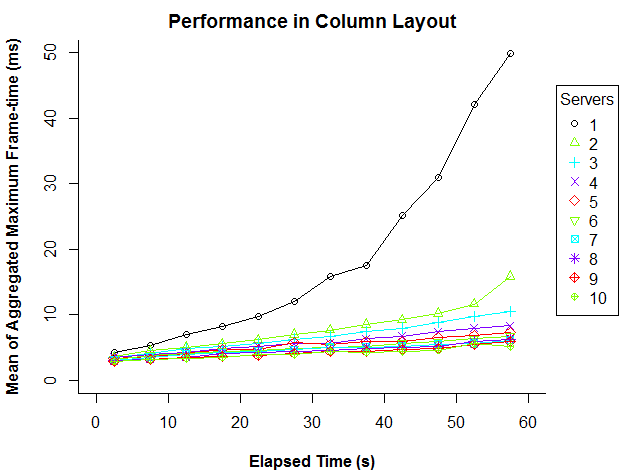
\includegraphics[width=\textwidth]{ColPerformance}
	\caption{Performance of increasing numbers of servers with an accumulating number of objects (in column layout)}
	\label{fig_PerCol}
\end{figure}

Experiments were also carried out using servers in a corner layout. The layouts of 3 and 4 servers are shown in Fig. \ref{ServerCorner}, in which the 4 server case is a 2x2 grid with a single corner intersection in the centre. The 9 server case is a 3x3 grid with 4 corner intersections. Injection rates and volume dimensions remain the same as in the column based experiments. Fig. \ref{fig_PerCor} shows the graph illustrating performance. The graph demonstrates that increasing the number of servers lowers the frame time. The additional processing overhead of exchanging more messages with more neighbouring servers in the 9 server experiment is outweighed by the performance gains of additional servers.

From these observations it may be declared that this system is scalable in corner configuration as the addition of servers results in increased performance.

\begin{figure}[!t]
	\begin{subfigure}{.5\textwidth}
		\begin{tikzpicture}[line cap=round,line join=round,>=triangle 45,x=1cm,y=1cm,scale=1.2]
		%	\clip(-3,-1.5) rectangle (3,3);
		\fill[line width=0.8pt,color=rvwvcq,fill=rvwvcq,fill opacity=0.1] (-1,-0.02) -- (1,-0.02) -- (1,-0.22) -- (-1,-0.22) -- cycle;
		\fill[line width=0.8pt,color=rvwvcq,fill=rvwvcq,fill opacity=0.1] (-0.02,2.5) -- (-0.02,0.5) -- (-0.22,0.5) -- (-0.22,2.5) -- cycle;
		\fill[line width=0.8pt,color=rvwvcq,fill=rvwvcq,fill opacity=0.1] (0.22,2.5) -- (0.22,0.5) -- (0.02,0.5) -- (0.02,2.5) -- cycle;
		\fill[line width=0.8pt,color=rvwvcq,fill=rvwvcq,fill opacity=0.1] (-2.5,0.22) -- (-0.5,0.22) -- (-0.5,0.02) -- (-2.5,0.02) -- cycle;
		\fill[line width=0.8pt,color=rvwvcq,fill=rvwvcq,fill opacity=0.1] (0.5,0.22) -- (2.5,0.22) -- (2.5,0.022) -- (0.5,0.022) -- cycle;
		\fill[line width=0.8pt,color=sim,fill=sim,fill opacity=0.1] (-3,3) -- (-3,-2) -- (3,-2) -- (3,3) -- cycle;
		\draw [line width=2pt] (-3,0)-- (3,0);
		\draw [line width=2pt] (0,3)-- (0,0);
		\draw [line width=0.8pt,color=rvwvcq] (-1,-0.02)-- (1,-0.02);
		\draw [line width=0.8pt,color=rvwvcq] (1,-0.02)-- (1,-0.22);
		\draw [line width=0.8pt,color=rvwvcq] (1,-0.22)-- (-1,-0.22);
		\draw [line width=0.8pt,color=rvwvcq] (-1,-0.22)-- (-1,-0.02);
		\draw [line width=0.8pt,color=rvwvcq] (-0.02,2.5)-- (-0.02,0.5);
		\draw [line width=0.8pt,color=rvwvcq] (-0.02,0.5)-- (-0.22,0.5);
		\draw [line width=0.8pt,color=rvwvcq] (-0.22,0.5)-- (-0.22,2.5);
		\draw [line width=0.8pt,color=rvwvcq] (-0.22,2.5)-- (-0.02,2.5);
		\draw [line width=0.8pt,color=rvwvcq] (0.22,2.5)-- (0.22,0.5);
		\draw [line width=0.8pt,color=rvwvcq] (0.22,0.5)-- (0.02,0.5);
		\draw [line width=0.8pt,color=rvwvcq] (0.02,0.5)-- (0.02,2.5);
		\draw [line width=0.8pt,color=rvwvcq] (0.02,2.5)-- (0.22,2.5);
		\draw (-1.5,2.5) node[anchor=center] {Server 0};
		\draw (1.5,2.5) node[anchor=center] {Server 1};
		\draw (0,-1) node[anchor=center] {Server 2};
		\draw [line width=0.8pt,color=rvwvcq] (-2.5,0.22)-- (-0.5,0.22);
		\draw [line width=0.8pt,color=rvwvcq] (-0.5,0.22)-- (-0.5,0.02);
		\draw [line width=0.8pt,color=rvwvcq] (-0.5,0.02)-- (-2.5,0.02);
		\draw [line width=0.8pt,color=rvwvcq] (-2.5,0.02)-- (-2.5,0.22);
		\draw [line width=0.8pt,color=rvwvcq] (0.5,0.22)-- (2.5,0.22);
		\draw [line width=0.8pt,color=rvwvcq] (2.5,0.22)-- (2.5,0.022);
		\draw [line width=0.8pt,color=rvwvcq] (2.5,0.022)-- (0.5,0.022);
		\draw [line width=0.8pt,color=rvwvcq] (0.5,0.022)-- (0.5,0.22);
		\draw [line width=0.8pt,color=rvwvcq] (-1.4,1.6)-- (-1.4,1.4);
		\draw [line width=0.8pt,color=rvwvcq] (-1.4,1.4)-- (-1.6,1.4);
		\draw [line width=0.8pt,color=rvwvcq] (-1.6,1.4)-- (-1.6,1.6);
		\draw [line width=0.8pt,color=rvwvcq] (-1.6,1.6)-- (-1.4,1.6);
		\draw [line width=0.8pt,color=rvwvcq] (1.6,1.6)-- (1.6,1.4);
		\draw [line width=0.8pt,color=rvwvcq] (1.6,1.4)-- (1.4,1.4);
		\draw [line width=0.8pt,color=rvwvcq] (1.4,1.4)-- (1.4,1.6);
		\draw [line width=0.8pt,color=rvwvcq] (1.4,1.6)-- (1.6,1.6);
		
		\draw [line width=0.8pt,color=rvwvcq] (0.1,-1.6)-- (0.1,-1.4);
		\draw [line width=0.8pt,color=rvwvcq] (0.1,-1.4)-- (-0.1,-1.4);
		\draw [line width=0.8pt,color=rvwvcq] (-0.1,-1.4)-- (-0.1,-1.6);
		\draw [line width=0.8pt,color=rvwvcq] (-0.1,-1.6)-- (0.1,-1.6);
		\end{tikzpicture}
		\centering
		\begin{tikzpicture}[line cap=round,line join=round,>=triangle 45,x=1cm,y=1cm]
		%		\clip(-3.661612836111066,-0.55) rectangle (6.690195527240868,1.05);
		\fill[line width=0.8pt,color=rvwvcq,fill=rvwvcq,fill opacity=0.1] (-2.5,0.22) -- (-2.3,0.22) -- (-2.3,0.02) -- (-2.5,0.02) -- cycle;
		\draw [line width=0.8pt,color=rvwvcq] (-2.5,0.22)-- (-2.3,0.22);
		\draw [line width=0.8pt,color=rvwvcq] (-2.3,0.22)-- (-2.3,0.02);
		\draw [line width=0.8pt,color=rvwvcq] (-2.3,0.02)-- (-2.5,0.02);
		\draw [line width=0.8pt,color=rvwvcq] (-2.5,0.02)-- (-2.5,0.22);
		\draw [line width=2pt] (-2.5,0.5)-- (-2.3,0.5);
		\draw (-2.1,0.5) node[anchor=west] {Region Boundary};
		\draw (-2.1,0.1) node[anchor=west] {Injection Volume};
		\end{tikzpicture}
		\caption{3 Server Corner Layout}
		\label{3ServerCorner}
	\end{subfigure}%
	\begin{subfigure}{.5\textwidth}
		\begin{tikzpicture}[line cap=round,line join=round,>=triangle 45,x=1cm,y=1cm,scale=1.2]
		%	\clip(-3,-3) rectangle (3,3);
		\fill[line width=0.8pt,color=rvwvcq,fill=rvwvcq,fill opacity=0.1] (0.5,-0.02) -- (2.5,-0.02) -- (2.5,-0.22) -- (0.5,-0.22) -- cycle;
		\fill[line width=0.8pt,color=rvwvcq,fill=rvwvcq,fill opacity=0.1] (-0.02,2.5) -- (-0.02,0.5) -- (-0.22,0.5) -- (-0.22,2.5) -- cycle;
		\fill[line width=0.8pt,color=rvwvcq,fill=rvwvcq,fill opacity=0.1] (0.22,2.5) -- (0.22,0.5) -- (0.02,0.5) -- (0.02,2.5) -- cycle;
		\fill[line width=0.8pt,color=rvwvcq,fill=rvwvcq,fill opacity=0.1] (-2.5,0.22) -- (-0.5,0.22) -- (-0.5,0.02) -- (-2.5,0.02) -- cycle;
		\fill[line width=0.8pt,color=rvwvcq,fill=rvwvcq,fill opacity=0.1] (0.5,0.22) -- (2.5,0.22) -- (2.5,0.022) -- (0.5,0.022) -- cycle;
		\fill[line width=0.8pt,color=rvwvcq,fill=rvwvcq,fill opacity=0.1] (-0.02,-0.5) -- (-0.02,-2.5) -- (-0.22,-2.5) -- (-0.22,-0.5) -- cycle;
		\fill[line width=0.8pt,color=rvwvcq,fill=rvwvcq,fill opacity=0.1] (0.22,-0.5) -- (0.22,-2.5) -- (0.02,-2.5) -- (0.02,-0.5) -- cycle;
		\fill[line width=0.8pt,color=rvwvcq,fill=rvwvcq,fill opacity=0.1] (-2.5,-0.022) -- (-0.5,-0.022) -- (-0.5,-0.22) -- (-2.5,-0.22) -- cycle;
		\fill[line width=0.8pt,color=sim,fill=sim,fill opacity=0.1] (-3,3) -- (-3,-3) -- (3,-3) -- (3,3) -- cycle;
		\draw [line width=2pt] (-3,0)-- (3,0);
		\draw [line width=2pt] (0,3)-- (0,0);
		\draw [line width=0.8pt,color=rvwvcq] (0.5,-0.02)-- (2.5,-0.02);
		\draw [line width=0.8pt,color=rvwvcq] (2.5,-0.02)-- (2.5,-0.22);
		\draw [line width=0.8pt,color=rvwvcq] (2.5,-0.22)-- (0.5,-0.22);
		\draw [line width=0.8pt,color=rvwvcq] (0.5,-0.22)-- (0.5,-0.02);
		\draw [line width=0.8pt,color=rvwvcq] (-0.02,2.5)-- (-0.02,0.5);
		\draw [line width=0.8pt,color=rvwvcq] (-0.02,0.5)-- (-0.22,0.5);
		\draw [line width=0.8pt,color=rvwvcq] (-0.22,0.5)-- (-0.22,2.5);
		\draw [line width=0.8pt,color=rvwvcq] (-0.22,2.5)-- (-0.02,2.5);
		\draw [line width=0.8pt,color=rvwvcq] (0.22,2.5)-- (0.22,0.5);
		\draw [line width=0.8pt,color=rvwvcq] (0.22,0.5)-- (0.02,0.5);
		\draw [line width=0.8pt,color=rvwvcq] (0.02,0.5)-- (0.02,2.5);
		\draw [line width=0.8pt,color=rvwvcq] (0.02,2.5)-- (0.22,2.5);
		\draw (-1.5,2.5) node[anchor=center] {Server 0};
		\draw (1.5,2.5) node[anchor=center] {Server 1};
		\draw (-1.5,-2.5) node[anchor=center] {Server 2};
		\draw (1.5,-2.5) node[anchor=center] {Server 3};
		\draw [line width=0.8pt,color=rvwvcq] (-2.5,0.22)-- (-0.5,0.22);
		\draw [line width=0.8pt,color=rvwvcq] (-0.5,0.22)-- (-0.5,0.02);
		\draw [line width=0.8pt,color=rvwvcq] (-0.5,0.02)-- (-2.5,0.02);
		\draw [line width=0.8pt,color=rvwvcq] (-2.5,0.02)-- (-2.5,0.22);
		\draw [line width=0.8pt,color=rvwvcq] (0.5,0.22)-- (2.5,0.22);
		\draw [line width=0.8pt,color=rvwvcq] (2.5,0.22)-- (2.5,0.022);
		\draw [line width=0.8pt,color=rvwvcq] (2.5,0.022)-- (0.5,0.022);
		\draw [line width=0.8pt,color=rvwvcq] (0.5,0.022)-- (0.5,0.22);
		\draw [line width=0.8pt,color=rvwvcq] (-0.02,-0.5)-- (-0.02,-2.5);
		\draw [line width=0.8pt,color=rvwvcq] (-0.02,-2.5)-- (-0.22,-2.5);
		\draw [line width=0.8pt,color=rvwvcq] (-0.22,-2.5)-- (-0.22,-0.5);
		\draw [line width=0.8pt,color=rvwvcq] (-0.22,-0.5)-- (-0.02,-0.5);
		\draw [line width=0.8pt,color=rvwvcq] (0.22,-0.5)-- (0.22,-2.5);
		\draw [line width=0.8pt,color=rvwvcq] (0.22,-2.5)-- (0.02,-2.5);
		\draw [line width=0.8pt,color=rvwvcq] (0.02,-2.5)-- (0.02,-0.5);
		\draw [line width=0.8pt,color=rvwvcq] (0.02,-0.5)-- (0.22,-0.5);
		\draw [line width=2pt] (0,0)-- (0,-3);
		\draw [line width=0.8pt,color=rvwvcq] (-2.5,-0.022)-- (-0.5,-0.022);
		\draw [line width=0.8pt,color=rvwvcq] (-0.5,-0.022)-- (-0.5,-0.22);
		\draw [line width=0.8pt,color=rvwvcq] (-0.5,-0.22)-- (-2.5,-0.22);
		\draw [line width=0.8pt,color=rvwvcq] (-2.5,-0.22)-- (-2.5,-0.022);
		\draw [line width=0.8pt,color=rvwvcq] (-1.4,1.6)-- (-1.4,1.4);
		\draw [line width=0.8pt,color=rvwvcq] (-1.4,1.4)-- (-1.6,1.4);
		\draw [line width=0.8pt,color=rvwvcq] (-1.6,1.4)-- (-1.6,1.6);
		\draw [line width=0.8pt,color=rvwvcq] (-1.6,1.6)-- (-1.4,1.6);
		\draw [line width=0.8pt,color=rvwvcq] (1.6,1.6)-- (1.6,1.4);
		\draw [line width=0.8pt,color=rvwvcq] (1.6,1.4)-- (1.4,1.4);
		\draw [line width=0.8pt,color=rvwvcq] (1.4,1.4)-- (1.4,1.6);
		\draw [line width=0.8pt,color=rvwvcq] (1.4,1.6)-- (1.6,1.6);
		
		\draw [line width=0.8pt,color=rvwvcq] (-1.4,-1.6)-- (-1.4,-1.4);
		\draw [line width=0.8pt,color=rvwvcq] (-1.4,-1.4)-- (-1.6,-1.4);
		\draw [line width=0.8pt,color=rvwvcq] (-1.6,-1.4)-- (-1.6,-1.6);
		\draw [line width=0.8pt,color=rvwvcq] (-1.6,-1.6)-- (-1.4,-1.6);
		\draw [line width=0.8pt,color=rvwvcq] (1.6,-1.6)-- (1.6,-1.4);
		\draw [line width=0.8pt,color=rvwvcq] (1.6,-1.4)-- (1.4,-1.4);
		\draw [line width=0.8pt,color=rvwvcq] (1.4,-1.4)-- (1.4,-1.6);
		\draw [line width=0.8pt,color=rvwvcq] (1.4,-1.6)-- (1.6,-1.6);
		\end{tikzpicture}
		\centering
		\caption{4 Server Corner Layout}
		\label{4ServerCorner}
	\end{subfigure}
\caption{Corner Layouts}
\label{ServerCorner}
\end{figure}

\begin{figure}[!t]
	\begin{tikzpicture}[line cap=round,line join=round,>=triangle 45,x=1cm,y=1cm]
	\fill[line width=0.8pt,color=sim,fill=sim,fill opacity=0.1] (-3,3) -- (-3,-6) -- (6,-6) -- (6,3) -- cycle;
	\draw [line width=2pt] (-3,0)-- (6,0);
	\draw [line width=2pt] (0,3)-- (0,-6);
	\draw [line width=2pt] (-3,-3)-- (6,-3);
	\draw [line width=2pt] (3,3)-- (3,-6);
	\draw (-1.5,2.5) node[anchor=center] {Server 0};
	\draw (1.5,2.5) node[anchor=center] {Server 1};
	\draw (4.5,2.5) node[anchor=center] {Server 2};
	\draw (-1.5,-0.5) node[anchor=center] {Server 3};
	\draw (1.5,-0.5) node[anchor=center] {Server 4};
	\draw (4.5,-0.5) node[anchor=center] {Server 5};
	\draw (-1.5,-3.5) node[anchor=center] {Server 6};
	\draw (1.5,-3.5) node[anchor=center] {Server 7};
	\draw (4.5,-3.5) node[anchor=center] {Server 8};
	
	%Injection volume
	% 4 -> 1
	\fill[line width=0.8pt,color=rvwvcq,fill=rvwvcq,fill opacity=0.1] (0.5,-0.02) -- (2.5,-0.02) -- (2.5,-0.22) -- (0.5,-0.22) -- cycle;
	% 0 -> 1
	\fill[line width=0.8pt,color=rvwvcq,fill=rvwvcq,fill opacity=0.1] (-0.02,2.5) -- (-0.02,0.5) -- (-0.22,0.5) -- (-0.22,2.5) -- cycle;
	% 1 -> 0
	\fill[line width=0.8pt,color=rvwvcq,fill=rvwvcq,fill opacity=0.1] (0.22,2.5) -- (0.22,0.5) -- (0.02,0.5) -- (0.02,2.5) -- cycle;
	% 0 -> 3
	\fill[line width=0.8pt,color=rvwvcq,fill=rvwvcq,fill opacity=0.1] (-2.5,0.22) -- (-0.5,0.22) -- (-0.5,0.02) -- (-2.5,0.02) -- cycle;
	% 1 -> 4
	\fill[line width=0.8pt,color=rvwvcq,fill=rvwvcq,fill opacity=0.1] (0.5,0.22) -- (2.5,0.22) -- (2.5,0.022) -- (0.5,0.022) -- cycle;
	% 3 -> 4
	\fill[line width=0.8pt,color=rvwvcq,fill=rvwvcq,fill opacity=0.1] (-0.02,-0.5) -- (-0.02,-2.5) -- (-0.22,-2.5) -- (-0.22,-0.5) -- cycle;
	% 4 -> 3
	\fill[line width=0.8pt,color=rvwvcq,fill=rvwvcq,fill opacity=0.1] (0.22,-0.5) -- (0.22,-2.5) -- (0.02,-2.5) -- (0.02,-0.5) -- cycle;
	% 3 -> 0
	\fill[line width=0.8pt,color=rvwvcq,fill=rvwvcq,fill opacity=0.1] (-2.5,-0.022) -- (-0.5,-0.022) -- (-0.5,-0.22) -- (-2.5,-0.22) -- cycle;
	
	% 5 -> 2
	\fill[line width=0.8pt,color=rvwvcq,fill=rvwvcq,fill opacity=0.1] (3.5,-0.02) -- (5.5,-0.02) -- (5.5,-0.22) -- (3.5,-0.22) -- cycle;
	% 6 -> 3
	\fill[line width=0.8pt,color=rvwvcq,fill=rvwvcq,fill opacity=0.1] (-2.5,-3.022) -- (-0.5,-3.022) -- (-0.5,-3.22) -- (-2.5,-3.22) -- cycle;
	% 7 -> 4
	\fill[line width=0.8pt,color=rvwvcq,fill=rvwvcq,fill opacity=0.1] (0.5,-3.022) -- (2.5,-3.022) -- (2.5,-3.22) -- (0.5,-3.22) -- cycle;
	% 8 -> 5
	\fill[line width=0.8pt,color=rvwvcq,fill=rvwvcq,fill opacity=0.1] (3.5,-3.022) -- (5.5,-3.022) -- (5.5,-3.22) -- (3.5,-3.22) -- cycle;
	% 2 -> 5
	\fill[line width=0.8pt,color=rvwvcq,fill=rvwvcq,fill opacity=0.1] (3.5,0.22) -- (5.5,0.22) -- (5.5,0.022) -- (3.5,0.022) -- cycle;
	% 3 -> 6
	\fill[line width=0.8pt,color=rvwvcq,fill=rvwvcq,fill opacity=0.1] (-2.5,-2.78) -- (-0.5,-2.78) -- (-0.5,-2.978) -- (-2.5,-2.978) -- cycle;
	% 4 -> 7
	\fill[line width=0.8pt,color=rvwvcq,fill=rvwvcq,fill opacity=0.1] (0.5,-2.78) -- (2.5,-2.78) -- (2.5,-2.978) -- (0.5,-2.978) -- cycle;
	% 5 -> 8
	\fill[line width=0.8pt,color=rvwvcq,fill=rvwvcq,fill opacity=0.1] (3.5,-2.78) -- (5.5,-2.78) -- (5.5,-2.978) -- (3.5,-2.978) -- cycle;
	% 1 -> 2
	\fill[line width=0.8pt,color=rvwvcq,fill=rvwvcq,fill opacity=0.1] (2.978,2.5) -- (2.978,0.5) -- (2.78,0.5) -- (2.78,2.5) -- cycle;
	% 4 -> 5
	\fill[line width=0.8pt,color=rvwvcq,fill=rvwvcq,fill opacity=0.1] (2.978,-0.5) -- (2.978,-2.5) -- (2.78,-2.5) -- (2.78,-0.5) -- cycle;
	% 6 -> 7
	\fill[line width=0.8pt,color=rvwvcq,fill=rvwvcq,fill opacity=0.1] (-0.02,-3.5) -- (-0.02,-5.5) -- (-0.22,-5.5) -- (-0.22,-3.5) -- cycle;
	% 7 -> 8
	\fill[line width=0.8pt,color=rvwvcq,fill=rvwvcq,fill opacity=0.1] (2.978,-3.5) -- (2.978,-5.5) -- (2.78,-5.5) -- (2.78,-3.5) -- cycle;
	% 7 -> 6
	\fill[line width=0.8pt,color=rvwvcq,fill=rvwvcq,fill opacity=0.1] (0.22,-3.5) -- (0.22,-5.5) -- (0.02,-5.5) -- (0.02,-3.5) -- cycle;
	% 2 -> 1
	\fill[line width=0.8pt,color=rvwvcq,fill=rvwvcq,fill opacity=0.1] (3.22,2.5) -- (3.22,0.5) -- (3.02,0.5) -- (3.02,2.5) -- cycle;
	% 5 -> 4
	\fill[line width=0.8pt,color=rvwvcq,fill=rvwvcq,fill opacity=0.1] (3.22,-0.5) -- (3.22,-2.5) -- (3.02,-2.5) -- (3.02,-0.5) -- cycle;
	% 8 -> 7
	\fill[line width=0.8pt,color=rvwvcq,fill=rvwvcq,fill opacity=0.1] (3.22,-3.5) -- (3.22,-5.5) -- (3.02,-5.5) -- (3.02,-3.5) -- cycle;
	
	
	% 4 -> 1
	\draw [line width=0.8pt,color=rvwvcq] (0.5,-0.02)-- (2.5,-0.02);
	\draw [line width=0.8pt,color=rvwvcq] (2.5,-0.02)-- (2.5,-0.22);
	\draw [line width=0.8pt,color=rvwvcq] (2.5,-0.22)-- (0.5,-0.22);
	\draw [line width=0.8pt,color=rvwvcq] (0.5,-0.22)-- (0.5,-0.02);
	
	% 5 -> 2
	\draw [line width=0.8pt,color=rvwvcq] (3.5,-0.02)-- (5.5,-0.02);
	\draw [line width=0.8pt,color=rvwvcq] (5.5,-0.02)-- (5.5,-0.22);
	\draw [line width=0.8pt,color=rvwvcq] (5.5,-0.22)-- (3.5,-0.22);
	\draw [line width=0.8pt,color=rvwvcq] (3.5,-0.22)-- (3.5,-0.02);
	
	% 0 -> 1
	\draw [line width=0.8pt,color=rvwvcq] (-0.02,2.5)-- (-0.02,0.5);
	\draw [line width=0.8pt,color=rvwvcq] (-0.02,0.5)-- (-0.22,0.5);
	\draw [line width=0.8pt,color=rvwvcq] (-0.22,0.5)-- (-0.22,2.5);
	\draw [line width=0.8pt,color=rvwvcq] (-0.22,2.5)-- (-0.02,2.5);
	
	% 1 -> 2
	\draw [line width=0.8pt,color=rvwvcq] (2.98,2.5)-- (2.98,0.5);
	\draw [line width=0.8pt,color=rvwvcq] (2.98,0.5)-- (2.78,0.5);
	\draw [line width=0.8pt,color=rvwvcq] (2.78,0.5)-- (2.78,2.5);
	\draw [line width=0.8pt,color=rvwvcq] (2.78,2.5)-- (2.98,2.5);
	
	% 1 -> 0
	\draw [line width=0.8pt,color=rvwvcq] (0.22,2.5)-- (0.22,0.5);
	\draw [line width=0.8pt,color=rvwvcq] (0.22,0.5)-- (0.02,0.5);
	\draw [line width=0.8pt,color=rvwvcq] (0.02,0.5)-- (0.02,2.5);
	\draw [line width=0.8pt,color=rvwvcq] (0.02,2.5)-- (0.22,2.5);
	
	% 2 -> 1
	\draw [line width=0.8pt,color=rvwvcq] (3.22,2.5)-- (3.22,0.5);
	\draw [line width=0.8pt,color=rvwvcq] (3.22,0.5)-- (3.02,0.5);
	\draw [line width=0.8pt,color=rvwvcq] (3.02,0.5)-- (3.02,2.5);
	\draw [line width=0.8pt,color=rvwvcq] (3.02,2.5)-- (3.22,2.5);
	
	% 0 -> 3
	\draw [line width=0.8pt,color=rvwvcq] (-2.5,0.22)-- (-0.5,0.22);
	\draw [line width=0.8pt,color=rvwvcq] (-0.5,0.22)-- (-0.5,0.02);
	\draw [line width=0.8pt,color=rvwvcq] (-0.5,0.02)-- (-2.5,0.02);
	\draw [line width=0.8pt,color=rvwvcq] (-2.5,0.02)-- (-2.5,0.22);
	
	% 1 -> 4
	\draw [line width=0.8pt,color=rvwvcq] (0.5,0.22)-- (2.5,0.22);
	\draw [line width=0.8pt,color=rvwvcq] (2.5,0.22)-- (2.5,0.022);
	\draw [line width=0.8pt,color=rvwvcq] (2.5,0.022)-- (0.5,0.022);
	\draw [line width=0.8pt,color=rvwvcq] (0.5,0.022)-- (0.5,0.22);
	
	% 2 -> 5
	\draw [line width=0.8pt,color=rvwvcq] (3.5,0.22)-- (5.5,0.22);
	\draw [line width=0.8pt,color=rvwvcq] (5.5,0.22)-- (5.5,0.022);
	\draw [line width=0.8pt,color=rvwvcq] (5.5,0.022)-- (3.5,0.022);
	\draw [line width=0.8pt,color=rvwvcq] (3.5,0.022)-- (3.5,0.22);
	
	% 3 -> 6
	\draw [line width=0.8pt,color=rvwvcq] (-2.5,-3.22)-- (-0.5,-3.22);
	\draw [line width=0.8pt,color=rvwvcq] (-0.5,-3.22)-- (-0.5,-3.02);
	\draw [line width=0.8pt,color=rvwvcq] (-0.5,-3.02)-- (-2.5,-3.02);
	\draw [line width=0.8pt,color=rvwvcq] (-2.5,-3.02)-- (-2.5,-3.22);
	
	% 4 -> 7
	\draw [line width=0.8pt,color=rvwvcq] (0.5,-3.22)-- (2.5,-3.22);
	\draw [line width=0.8pt,color=rvwvcq] (2.5,-3.22)-- (2.5,-3.022);
	\draw [line width=0.8pt,color=rvwvcq] (2.5,-3.022)-- (0.5,-3.022);
	\draw [line width=0.8pt,color=rvwvcq] (0.5,-3.022)-- (0.5,-3.22);
	
	% 5 -> 8
	\draw [line width=0.8pt,color=rvwvcq] (3.5,-3.22)-- (5.5,-3.22);
	\draw [line width=0.8pt,color=rvwvcq] (5.5,-3.22)-- (5.5,-3.022);
	\draw [line width=0.8pt,color=rvwvcq] (5.5,-3.022)-- (3.5,-3.022);
	\draw [line width=0.8pt,color=rvwvcq] (3.5,-3.022)-- (3.5,-3.22);
	
	% 3 -> 4
	\draw [line width=0.8pt,color=rvwvcq] (-0.02,-0.5)-- (-0.02,-2.5);
	\draw [line width=0.8pt,color=rvwvcq] (-0.02,-2.5)-- (-0.22,-2.5);
	\draw [line width=0.8pt,color=rvwvcq] (-0.22,-2.5)-- (-0.22,-0.5);
	\draw [line width=0.8pt,color=rvwvcq] (-0.22,-0.5)-- (-0.02,-0.5);
	
	% 4 -> 5
	\draw [line width=0.8pt,color=rvwvcq] (2.98,-0.5)-- (2.98,-2.5);
	\draw [line width=0.8pt,color=rvwvcq] (2.98,-2.5)-- (2.78,-2.5);
	\draw [line width=0.8pt,color=rvwvcq] (2.78,-2.5)-- (2.78,-0.5);
	\draw [line width=0.8pt,color=rvwvcq] (2.78,-0.5)-- (2.98,-0.5);
	
	% 6 -> 7
	\draw [line width=0.8pt,color=rvwvcq] (-0.02,-3.5)-- (-0.02,-5.5);
	\draw [line width=0.8pt,color=rvwvcq] (-0.02,-5.5)-- (-0.22,-5.5);
	\draw [line width=0.8pt,color=rvwvcq] (-0.22,-5.5)-- (-0.22,-3.5);
	\draw [line width=0.8pt,color=rvwvcq] (-0.22,-3.5)-- (-0.02,-3.5);
	
	% 7 -> 8
	\draw [line width=0.8pt,color=rvwvcq] (2.98,-3.5)-- (2.98,-5.5);
	\draw [line width=0.8pt,color=rvwvcq] (2.98,-5.5)-- (2.78,-5.5);
	\draw [line width=0.8pt,color=rvwvcq] (2.78,-5.5)-- (2.78,-3.5);
	\draw [line width=0.8pt,color=rvwvcq] (2.78,-3.5)-- (2.98,-3.5);
	
	% 4 -> 3
	\draw [line width=0.8pt,color=rvwvcq] (0.22,-0.5)-- (0.22,-2.5);
	\draw [line width=0.8pt,color=rvwvcq] (0.22,-2.5)-- (0.02,-2.5);
	\draw [line width=0.8pt,color=rvwvcq] (0.02,-2.5)-- (0.02,-0.5);
	\draw [line width=0.8pt,color=rvwvcq] (0.02,-0.5)-- (0.22,-0.5);
	
	% 5 -> 4
	\draw [line width=0.8pt,color=rvwvcq] (3.22,-0.5)-- (3.22,-2.5);
	\draw [line width=0.8pt,color=rvwvcq] (3.22,-2.5)-- (3.02,-2.5);
	\draw [line width=0.8pt,color=rvwvcq] (3.02,-2.5)-- (3.02,-0.5);
	\draw [line width=0.8pt,color=rvwvcq] (3.02,-0.5)-- (3.22,-0.5);
	
	% 3 -> 0
	\draw [line width=0.8pt,color=rvwvcq] (-2.5,-0.022)-- (-0.5,-0.022);
	\draw [line width=0.8pt,color=rvwvcq] (-0.5,-0.022)-- (-0.5,-0.22);
	\draw [line width=0.8pt,color=rvwvcq] (-0.5,-0.22)-- (-2.5,-0.22);
	\draw [line width=0.8pt,color=rvwvcq] (-2.5,-0.22)-- (-2.5,-0.022);
	
	% 7 -> 6
	\draw [line width=0.8pt,color=rvwvcq] (0.22,-3.5)-- (0.22,-5.5);
	\draw [line width=0.8pt,color=rvwvcq] (0.22,-5.5)-- (0.02,-5.5);
	\draw [line width=0.8pt,color=rvwvcq] (0.02,-5.5)-- (0.02,-3.5);
	\draw [line width=0.8pt,color=rvwvcq] (0.02,-3.5)-- (0.22,-3.5);
	
	% 8 -> 7
	\draw [line width=0.8pt,color=rvwvcq] (3.22,-3.5)-- (3.22,-5.5);
	\draw [line width=0.8pt,color=rvwvcq] (3.22,-5.5)-- (3.02,-5.5);
	\draw [line width=0.8pt,color=rvwvcq] (3.02,-5.5)-- (3.02,-3.5);
	\draw [line width=0.8pt,color=rvwvcq] (3.02,-3.5)-- (3.22,-3.5);
	
	% 3 -> 6
	\draw [line width=0.8pt,color=rvwvcq] (-2.5,-2.78)-- (-0.5,-2.78);
	\draw [line width=0.8pt,color=rvwvcq] (-0.5,-2.78)-- (-0.5,-2.978);
	\draw [line width=0.8pt,color=rvwvcq] (-0.5,-2.978)-- (-2.5,-2.978);
	\draw [line width=0.8pt,color=rvwvcq] (-2.5,-2.978)-- (-2.5,-2.78);
	
	% 4 -> 7
	\draw [line width=0.8pt,color=rvwvcq] (0.5,-2.78)-- (2.5,-2.78);
	\draw [line width=0.8pt,color=rvwvcq] (2.5,-2.78)-- (2.5,-2.978);
	\draw [line width=0.8pt,color=rvwvcq] (2.5,-2.978)-- (0.5,-2.978);
	\draw [line width=0.8pt,color=rvwvcq] (0.5,-2.978)-- (0.5,-2.78);
	
	% 5 -> 8
	\draw [line width=0.8pt,color=rvwvcq] (3.5,-2.78)-- (5.5,-2.78);
	\draw [line width=0.8pt,color=rvwvcq] (5.5,-2.78)-- (5.5,-2.978);
	\draw [line width=0.8pt,color=rvwvcq] (5.5,-2.978)-- (3.5,-2.978);
	\draw [line width=0.8pt,color=rvwvcq] (3.5,-2.978)-- (3.5,-2.78);
	
	% Server 0
	\draw [line width=0.8pt,color=rvwvcq] (-1.4,1.6)-- (-1.4,1.4);
	\draw [line width=0.8pt,color=rvwvcq] (-1.4,1.4)-- (-1.6,1.4);
	\draw [line width=0.8pt,color=rvwvcq] (-1.6,1.4)-- (-1.6,1.6);
	\draw [line width=0.8pt,color=rvwvcq] (-1.6,1.6)-- (-1.4,1.6);
	
	% Server 1
	\draw [line width=0.8pt,color=rvwvcq] (1.6,1.6)-- (1.6,1.4);
	\draw [line width=0.8pt,color=rvwvcq] (1.6,1.4)-- (1.4,1.4);
	\draw [line width=0.8pt,color=rvwvcq] (1.4,1.4)-- (1.4,1.6);
	\draw [line width=0.8pt,color=rvwvcq] (1.4,1.6)-- (1.6,1.6);
	
	% Server 2
	\draw [line width=0.8pt,color=rvwvcq] (4.6,1.6)-- (4.6,1.4);
	\draw [line width=0.8pt,color=rvwvcq] (4.6,1.4)-- (4.4,1.4);
	\draw [line width=0.8pt,color=rvwvcq] (4.4,1.4)-- (4.4,1.6);
	\draw [line width=0.8pt,color=rvwvcq] (4.4,1.6)-- (4.6,1.6);
	
	% Server 3
	\draw [line width=0.8pt,color=rvwvcq] (-1.4,-1.6)-- (-1.4,-1.4);
	\draw [line width=0.8pt,color=rvwvcq] (-1.4,-1.4)-- (-1.6,-1.4);
	\draw [line width=0.8pt,color=rvwvcq] (-1.6,-1.4)-- (-1.6,-1.6);
	\draw [line width=0.8pt,color=rvwvcq] (-1.6,-1.6)-- (-1.4,-1.6);
	
	% Server 4
	\draw [line width=0.8pt,color=rvwvcq] (1.6,-1.6)-- (1.6,-1.4);
	\draw [line width=0.8pt,color=rvwvcq] (1.6,-1.4)-- (1.4,-1.4);
	\draw [line width=0.8pt,color=rvwvcq] (1.4,-1.4)-- (1.4,-1.6);
	\draw [line width=0.8pt,color=rvwvcq] (1.4,-1.6)-- (1.6,-1.6);
	
	% Server 5
	\draw [line width=0.8pt,color=rvwvcq] (4.6,-1.6)-- (4.6,-1.4);
	\draw [line width=0.8pt,color=rvwvcq] (4.6,-1.4)-- (4.4,-1.4);
	\draw [line width=0.8pt,color=rvwvcq] (4.4,-1.4)-- (4.4,-1.6);
	\draw [line width=0.8pt,color=rvwvcq] (4.4,-1.6)-- (4.6,-1.6);
	
	% Server 6
	\draw [line width=0.8pt,color=rvwvcq] (-1.4,-4.6)-- (-1.4,-4.4);
	\draw [line width=0.8pt,color=rvwvcq] (-1.4,-4.4)-- (-1.6,-4.4);
	\draw [line width=0.8pt,color=rvwvcq] (-1.6,-4.4)-- (-1.6,-4.6);
	\draw [line width=0.8pt,color=rvwvcq] (-1.6,-4.6)-- (-1.4,-4.6);
	
	% Server 7
	\draw [line width=0.8pt,color=rvwvcq] (1.6,-4.6)-- (1.6,-4.4);
	\draw [line width=0.8pt,color=rvwvcq] (1.6,-4.4)-- (1.4,-4.4);
	\draw [line width=0.8pt,color=rvwvcq] (1.4,-4.4)-- (1.4,-4.6);
	\draw [line width=0.8pt,color=rvwvcq] (1.4,-4.6)-- (1.6,-4.6);
	
	% Server 8
	\draw [line width=0.8pt,color=rvwvcq] (4.6,-4.6)-- (4.6,-4.4);
	\draw [line width=0.8pt,color=rvwvcq] (4.6,-4.4)-- (4.4,-4.4);
	\draw [line width=0.8pt,color=rvwvcq] (4.4,-4.4)-- (4.4,-4.6);
	\draw [line width=0.8pt,color=rvwvcq] (4.4,-4.6)-- (4.6,-4.6);
	
	\end{tikzpicture}
	\centering
	\begin{tikzpicture}[line cap=round,line join=round,>=triangle 45,x=1cm,y=1cm]
	\clip(-4,0) rectangle (7,1.5);
	\draw [line width=2pt] (-3.5,0.7)-- (-3.3,0.7);
	\draw (-3.1,0.7) node[anchor=west] {Server-Region Boundary};
	
	\fill[line width=0.8pt,color=rvwvcq,fill=rvwvcq,fill opacity=0.1] (2.5,0.82) -- (2.3,0.82) -- (2.3,0.62) -- (2.5,0.62) -- cycle;
	\draw [line width=0.8pt,color=rvwvcq] (2.5,0.82)-- (2.3,0.82);
	\draw [line width=0.8pt,color=rvwvcq] (2.3,0.82)-- (2.3,0.62);
	\draw [line width=0.8pt,color=rvwvcq] (2.3,0.62)-- (2.5,0.62);
	\draw [line width=0.8pt,color=rvwvcq] (2.5,0.62)-- (2.5,0.82);
	
	\draw (2.7,0.7) node[anchor=west] {Injection Volume};
	\end{tikzpicture}
	\caption{9 Server Corner Layout}
	\label{3x3Servers}
\end{figure}

\begin{figure}[!t]
	\centering
	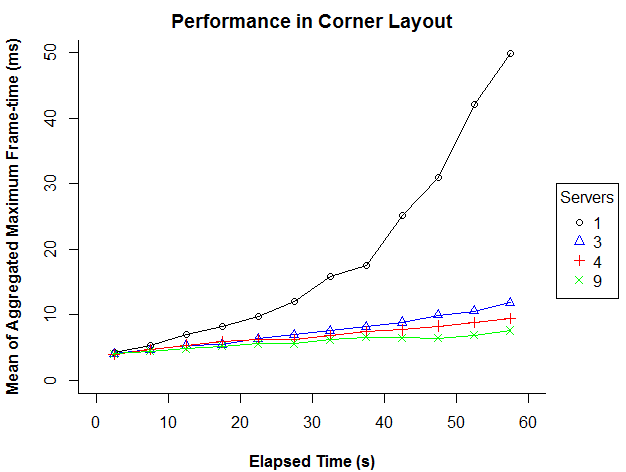
\includegraphics[width=\textwidth]{CorPerformance}
	\caption{Performance of increasing numbers of servers with an accumulating number of objects (in corner layout)}
	\label{fig_PerCor}
\end{figure}

\section{Collision Correctness Experiments}
In the following section the correctness of collisions between objects is explored, i.e. do objects have the same collision behaviour in a AP as they do in a centralised system.

The following points highlight the contributions of the correctness experiments:
\begin{itemize}
	\item Demonstrate that collisions between objects and migrating are handled correctly as long as the factors (speed, frame-time, latency) remain within their tolerances. Collisions can be handled correctly under worsening conditions (higher object speed, frame-time and latency), so long as the tolerances account for these.
	\item Demonstrate that late collisions begin to occur once tolerances are exceeded or as predicted by the aura calculation, i.e. auras are the size they need to be, and no larger, which would impact on performance.
	\item Demonstrate the severity of each of the factors being exceeded, i.e. when different factors are exceeded, how badly are collisions handled?
	\item Measure the frequency of two-object-thrashing
\end{itemize}

Experiments were undertaken to detect erroneous collisions under different conditions and are concerned with objects that are migrating and/or interacting with an object that has recently migrated. Erroneous collisions fall into two categories:
\begin{itemize}
	\item Missed collisions - collisions that should have taken place but were not detected by the physics engine e.g. Bullet through paper problem.
	\item Late collisions - collisions that were detected later than expected in a centralised simulation and result in not only different collision results, but also unstable collision response.
\end{itemize}

%To understand how late collisions lead to unstable collision response, we must first understand how in real-time collision detection works. In real-time physics engines, objects move in discrete steps, as a result of this, when two objects collide, they overlap each other i.e. penetrate. The collision is resolved by calculating the forces resulting from the collision and moving the objects so they no longer overlap (in PhysX if penetration is high, the latter may be done over several physics time-steps). If the penetration is high, such as in the case of a late collision response or if two objects are moving at high speed towards one another, the collision response can no longer guarantee stable results.

%It is possible to detect late collisions between objects. Given the relative speed of the two objects and the physics time-step, it possible to calculate the maximum expected penetration distance. If a collision is detected and it is above this value, it means it is a late collision.

%Maximum penetration for a given speed occurs when two objects travelling directly towards each other have, in the final time-step before colliding the two objects have no distance between them, but are not overlapping, so not colliding. The next physics time-step, the collision will be detected and will have the maximum penetration possible for that relative speed. Re-arranging $s=d/t$, to $d=s.t$ and substituting the physics time-step for $t$, gives us the maximum distance (penetration) for a relative speed, and we are able to plot the maximum expected penetration line.

%In real-time physics, speed of calculation is favoured over accuracy of collision response, as a result of this 

%, this is known as the collision response (in real-time physics, speed of calculation is favoured over accuracy of collision response). High collision penetration e.g. if two objects are moving quickly towards one another, can lead to unstable collision response, which is undesirable.

%Experiments were carried out where collision results were recorded and used to detect missed and late collisions of objects. The experiment scenario used only two objects, meaning if there was a missed collision there would be no collision output. The two objects start the scenario with a specified velocity (drag and gravity are disabled), the direction being directly towards the other object and the two objects were given the same speed, which is varied throughout the experiment. Spheres were used, so rotational effects don't need to be accounted for.

A recap of how a naive system can lead to erroneous collision behaviour and how AP can lead to erroneous collision behaviour if speed, frame-time, or latency exceed the user-defined tolerances will now be given.

In a hypothetical naive system, a system that does not use AP, objects are migrated solely based on their position and objects on a remote server are not accounted for. Two objects close to the server region boundary could be occupying the same space at the same time. If one object were to be migrated to the other server, for example, if the centre of the object has traversed the region boundary, then the object would be migrated into an overlapping space as the other object on the receiving server. This penetration could be much greater than would be expected in a normal collision detection and could lead to a highly erroneous collision response.

AP works by predicting the future bounding sphere of both the object projecting the aura and a potential object on the remote server. When an object collides with an aura from a remote server, the object is migrated to the owner of the aura. However, the aura projection is not instantaneous and has to account for the following three factors: the speeds of both objects; the frame-times of the two servers; and the latency between the two servers. These three factors need to be known through the duration between the aura projection being initiated and a remote object being received and collided with. As it not possible to know these three factors in advance, tolerances must be used. These three tolerances are used to determine the size of the aura with the aim to ensure a remote object is migrated before a collision happens. If the speed tolerance is exceeded, an object can penetrate deeper into the aura than the maximum penetration to ensure it is migrated in time before a collision occurs. In the case of latency, the aura would potentially arrive too late on the receiving server, meaning the migration is triggered too late. In addition to this, the migrating object's arrival will be delayed, potentially leading to a late collision. In the case of frame-time, the extra delay between the messages being processed and physics time-step could cause the collision with the aura to be detected too late and potentially lead to a late collision. Furthermore, the extra delay between the migration message being received and the object being present in the physics simulation on the receiving server could cause the collision to be detected too late.

%TODO: Expand on late collisions producing different results?

%TODO: The following paragraph should probably be in a section about why late collisions are bad and why we want to avoid them.
To understand how late collisions lead to unstable collision response, it must first be understood how in real-time collision detection works, which is discussed in \ref{collision_detection}. In summary, in real-time physics engines, objects move in discrete steps. As a result of this, when two objects collide, they overlap each other i.e. penetrate. The collision is resolved by calculating the forces resulting from the collision and moving the objects so they no longer overlap (in PhysX if penetration is high, the latter may be done over several physics time-steps). If the penetration is high, such as in the case of a late collision response or if two objects are moving at high speed towards one another, the collision response can no longer guarantee stable results.

\subsection{Collision Error Detection}
It is possible to detect late collisions between objects; Given the relative speed of the two objects and the physics time-step, it is possible to calculate the maximum expected penetration distance. If a collision is detected and it is above this value, it means it is a late collision. In addition, if no collisions occur, it means there is a missed collision.

Collision penetration can range from 0 to maximum penetration distance and depends upon the distance between the two objects' surfaces in the time-step before the collision. Maximum penetration for a given speed occurs when two objects are travelling directly towards each other and in the time-step before the collision occurs, there is no distance between the surfaces of the objects. In the next time-step, this results in the two objects overlapping each other with the maximum penetration for their relative speed. The overlap is then detected as a collision by the physics engine. Re-arranging $s=d/t$, to $d=s.t$ and substituting the physics time-step for $t$, gives us the maximum distance (penetration) for a relative speed, and we are able to plot the maximum expected penetration line.

%In real-time physics, speed of calculation is favoured over accuracy of collision response, as a result of this 

%, this is known as the collision response (in real-time physics, speed of calculation is favoured over accuracy of collision response). High collision penetration e.g. if two objects are moving quickly towards one another, can lead to unstable collision response, which is undesirable.

%TODO: cite that deep penetration is bad

In all the following experiments collisions were recorded, for each collision, the following data is contained: Relative Speed, the speed of the two colliding objects relative to each other; Penetration, the distance the two objects overlapped when the collision was detected. PhysX reports penetration of collisions as negative values and can report collisions before the two objects are intersecting, which is recorded as a positive penetration. In all experiments, the penetration is negated for simplicity. The relative speed and penetration can be used to determine if the collision was a late collision. In all the following experimental scenarios only two objects are used, meaning if there was a missed collision there would be no collision output and multiple collisions from the same pair of objects can be ignored. The two objects start the scenario with a specified velocity (drag and gravity are disabled), the direction being directly towards the other object and the two objects were given the same speed and a random variation of between $0$ and $-1m\mathord{\cdot}s^{-1}$ to prevent identical results between iterations. Spheres were used, so rotational effects, such as rotational velocity, do not need to be accounted for. 

Thrashing between two objects on different servers is an unsolved problem in AP; thrashing occurrences can be detected by counting the number of migrations that occur before the first collision is detected, as only two objects are involved in each experiment, the number of migrations before a collision should only be one, otherwise thrashing has occurred. For the purposes of these experiments, collisions involving thrashing will be excluded, regardless of the correctness of the collision. For the remainder of this chapter, thrashing refers to only thrashing between two objects and not the solved 3-object-thrashing problem.

%TODO: Some justifcation for exluding thrashing?

\subsection{Control Experiment}

%\begin{figure}[t]
%	\centering
%	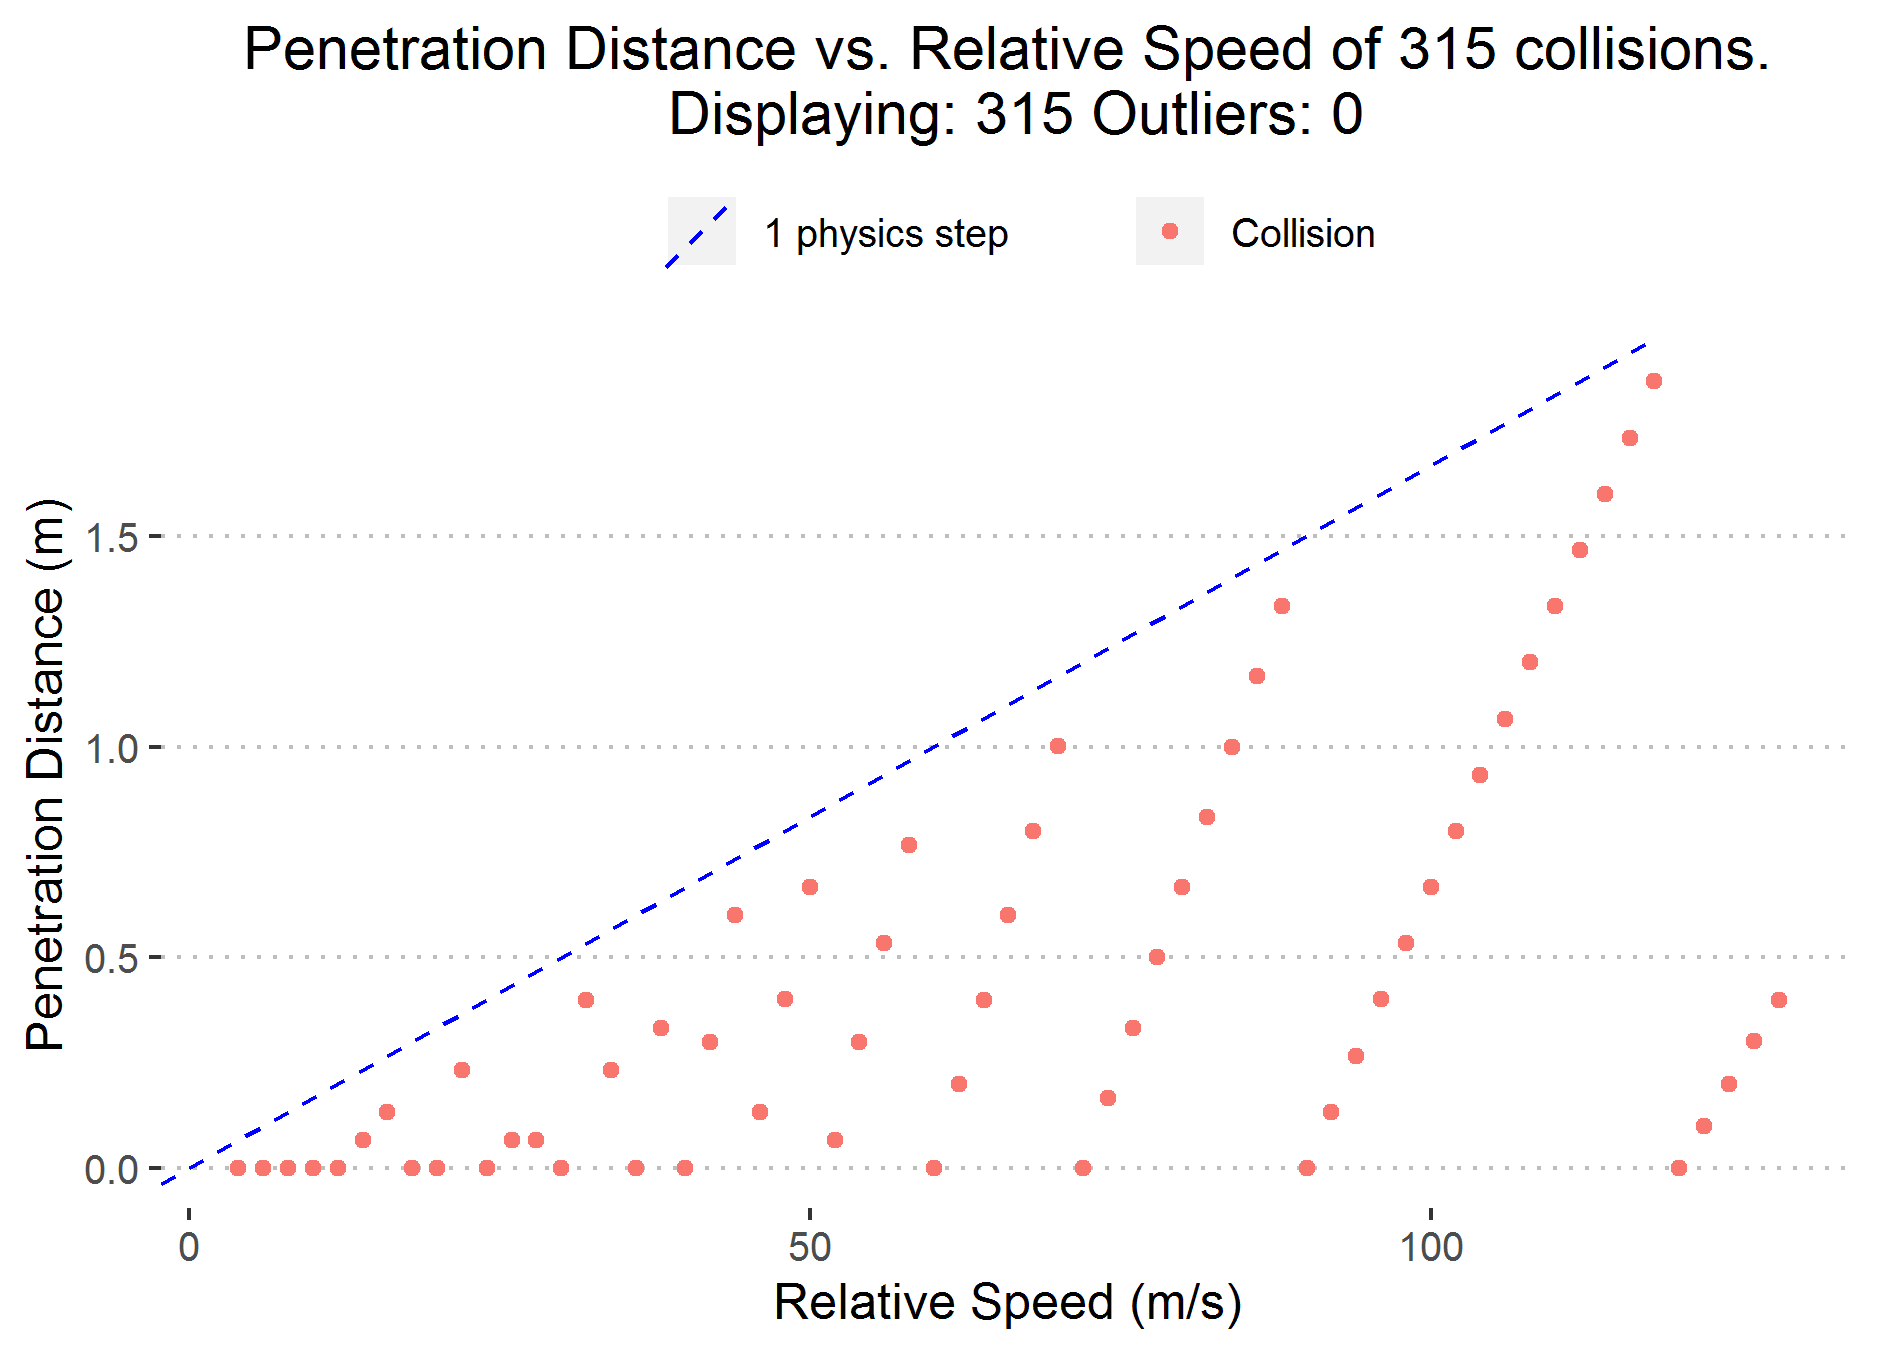
\includegraphics[width=\textwidth]{CentralCollisionsPenDistanceVsSpeed}
%	\caption{Penetration distance of collisions with varying speed. The maximum expected penetration distance of 1 physics step is marked with a dashed blue line.}
%	\label{fig_ErrorControlDistance}
%\end{figure}

\begin{figure}[t]
	\centering
	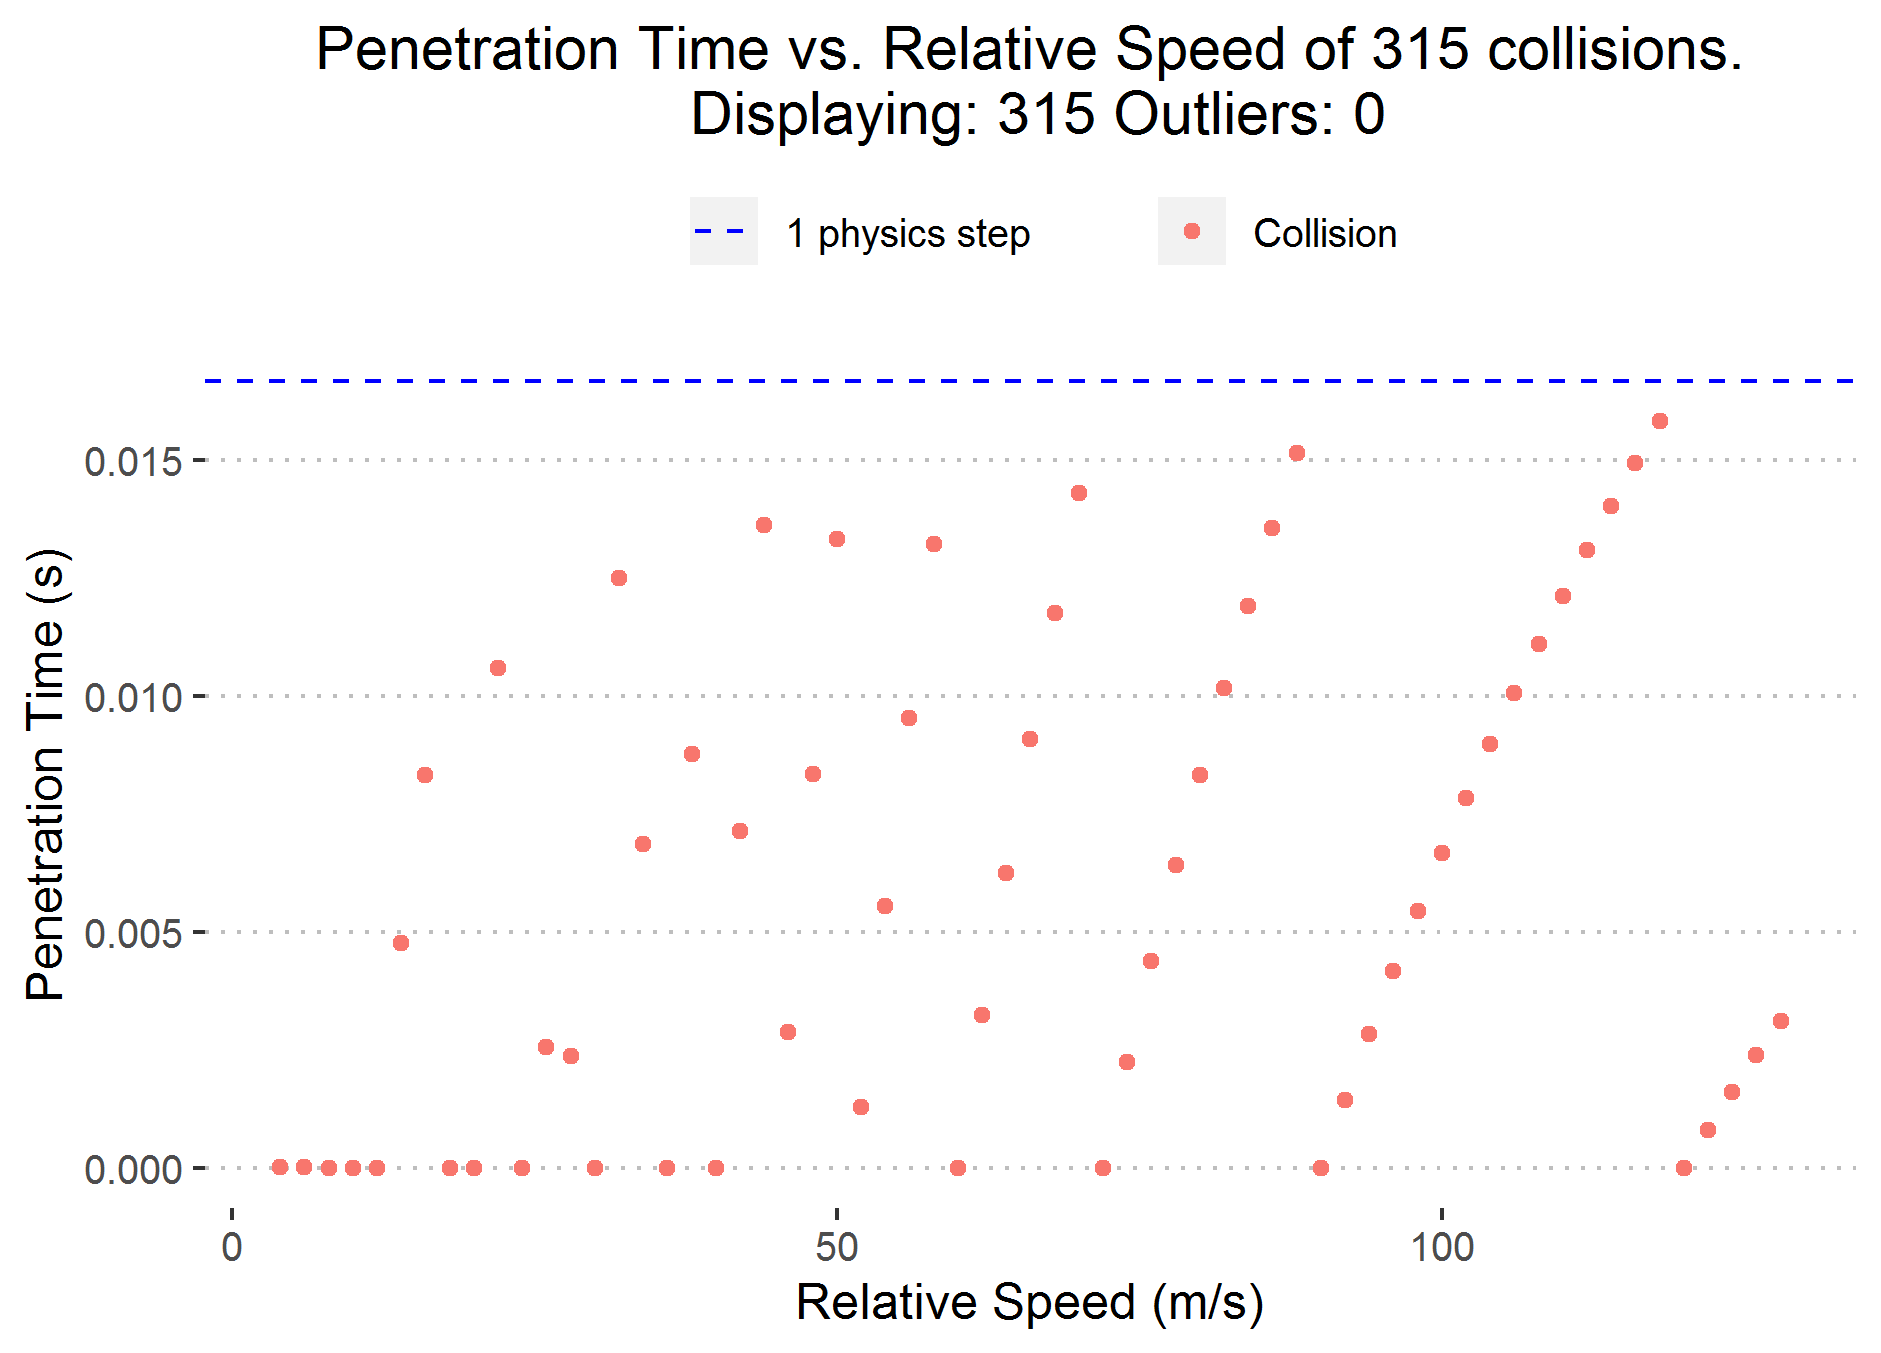
\includegraphics[width=\textwidth]{CentralCollisionsPenVsSpeed}
	\caption{Penetration time of collisions with varying speed. The maximum expected penetration time of 1 physics step is marked with a dashed blue line.}
	\label{fig_ErrorControlTime}
\end{figure}

A control experiment on a centralised system (single server, single simulation) was performed, in which the scenario was repeated multiple times. The speed of each object is increased from $1$ to $64m\mathord{\cdot}s^{-1}$ in steps of $1m\mathord{\cdot}s^{-1}$. The experiment was repeated $50$ times, for a total of $3150$ collisions. %Fig. \ref{fig_ErrorControlDistance} shows the penetration of objects with increasing speed in a centralised simulation and demonstrates that penetration distance is never greater than the maximum expected penetration. 

As speed increases, expected penetration increases. Using penetration time gives us a uniform maximum expected value regardless of speed.
Re-arranging $s=d/t$, to $t=d/s$ and substituting the collision penetration for $d$ and speed for $s$, gives us the penetration time for a collision. It should be noted that because physics engines work in discrete time steps, this time value does not actually reflect the real time the colliding objects were penetrating each other. It should also be noted that PhysX can report collisions before objects intersect, leading to the negative penetration distances shown. Correct collisions result in penetration times of up to 1 physics time step and any collision penetration times over this value are considered erroneous. Fig. \ref{fig_ErrorControlTime} shows the penetration of objects with increasing speed in a centralised simulation (displaying speed without the random variation) and demonstrates that penetration time is never greater than the time of one physics step, regardless of the relative speed of objects. The purpose of this experiment was to confirm the predicted maximum expected penetration in a centralised simulation. This provides a benchmark of correctness to compare with results from experiments using multiple servers.

Using the above method to detect late collisions, experiments on a distributed configuration of a simulation were then performed. Experiments were carried out for both variations in all three aura tolerance factors and packet-loss. Experiments were conducted using AWS G2.2xlarge servers located within the same geographical region. A G2.2xlarge instance uses a 2.60GHz Intel Xeon E5-2670 CPU with 16GB RAM and an NVIDIA GRID K520 (Kepler) GPU running Ubuntu 18.04 LTS.

\subsection{Experiment- Varying Factors}
Experiments were carried out to demonstrate the effects of varying each aura calculation factor on the correctness of collisions between objects. The purpose of these experiments is to demonstrate that collisions in AP are always correct if the three factors that determine aura size remain within respective tolerance, i.e. there are no late or missed collisions. In addition, if the aura calculation is correct, we expect to see late collisions begin to occur as soon as tolerances are exceeded. If errors do not occur as soon as the tolerances are exceeded, this is evidence that the aura radius is too large. Large auras can lead to reduced performance in AP, therefore auras that are only as large as needed to be, for the given tolerance, are desirable to maximise performance.

In order to rigorously test the hypothesis "Can real-time physics simulations remain correct when scaled?", a `worst-case' scenario was used for the experiments, in which two objects are moving directly towards each other and collide while one of the objects is intersecting the boundary between servers. This experiment setup is illustrated in Fig. \ref{fig_CorrectnessExperiment}. In this experiment two servers were used with one sphere being created on each server. The two spheres were given starting positions so the two would collide at a point when one of the spheres is intersecting the server region boundary, thus creating the most likely situation for spheres collide with each other in the first time-step after being migrated; this is necessary as AP can only lead to late or missed collisions when at least one sphere involved in the collision has just migrated (received since the last physics time-step). This is because non-migrating spheres behave the same as spheres in a centralised solution, therefore only collisions that involve a sphere that has just migrated are considered in the experiment results.

\begin{figure}
	\centering
	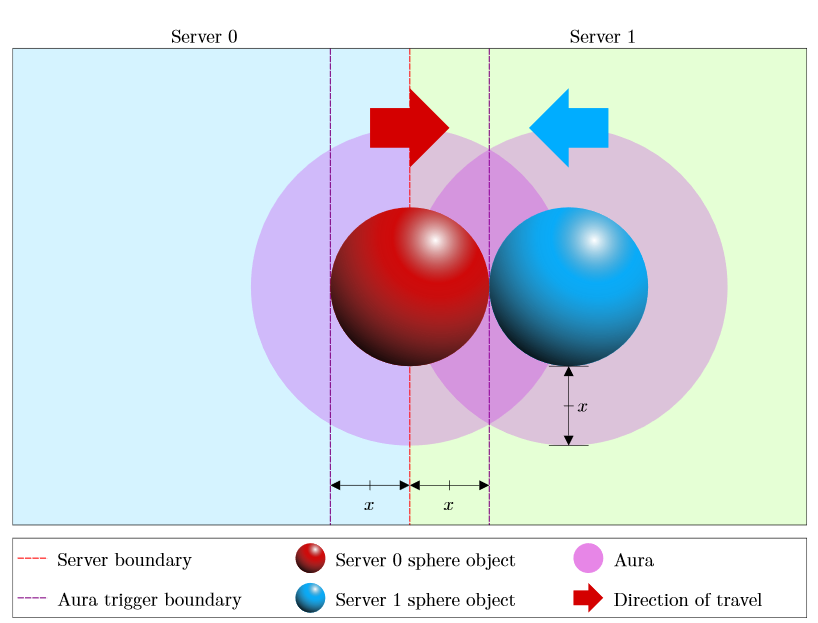
\includegraphics[width=0.9\textwidth]{CorrectnessExperiment}
	\caption{Correctness experiment setup. The setup is the `worst-case' scenario, in which two objects are moving directly towards each other and collide while one of the objects is intersecting the boundary between servers.}
	\label{fig_CorrectnessExperiment}
\end{figure}

There are three factors that are used to determine aura size: speed; latency; and frame-time. In order to demonstrate that collisions always remain correct when within their tolerance, even under worsening conditions and the effect each factor has on collision correctness, one aura factor is varied per experiment and the other two factors are set to equal the tolerance values. For example, speed is varied, the latency between the servers is set to equal the latency tolerance value and the frame-time of each server is set to equal the frame-time tolerance value. The non-varied factors are set to equal the tolerance values as exceeding the tolerance value in one factor can be compensated for by having a value below the tolerance in a different factor. For example, the latency may exceed the tolerance by $5ms$, but the frame-time could be more than $5ms$ below the frame-time tolerance and the collision would still be expected to be correctly handled by AP.

Speed is controlled such that the two objects used in the experiment collide with each other with that desired speed. Latency is controlled using the Traffic Control tool to emulate latency for all communications between the servers. The desired latency is applied as a fixed delay to each server, resulting in that delay being applied to all packets outgoing from that server. Frame-time is controlled using a wait within the simulation's update loop, which is limited to a target frame-time as the resultant frame-times are a normal distribution with the target frame-time as the median. This is illustrated in Fig. \ref{fig_FrameTimeDensity}. As a result of this, half of all frames are expected to be above the target frame-time, which may cause false-positives in detecting late collisions, in the following experiments. However, the following points should be considered: the variance in frame-time is low; longer frames have to occur exactly at the time of messages being exchanged; exceeding one factor can be compensated for by having a low value in another factor. Therefore, false-positives are expected to be rare up until the tolerance value is approached. It should be noted that variance increases with target frame-time, therefore more false-positives should expected with experiments using higher target frame-times.

\begin{figure}
	\centering
	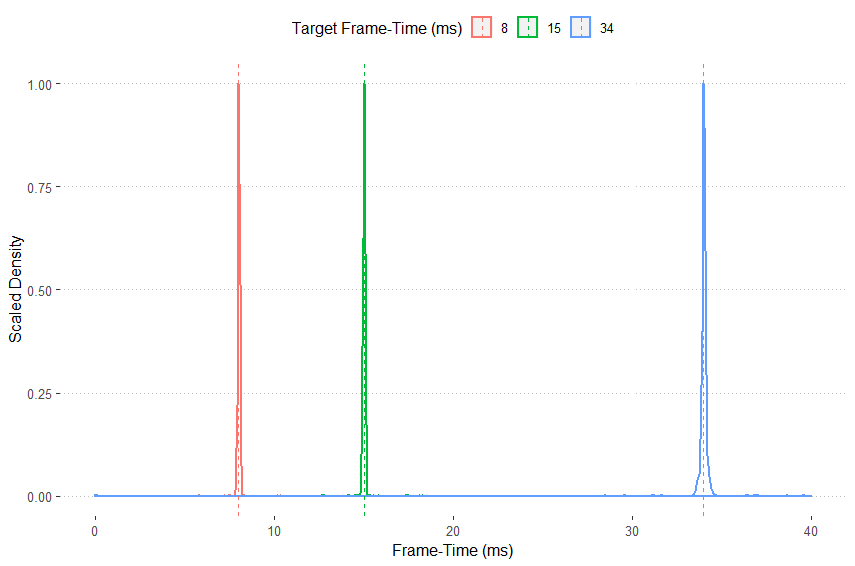
\includegraphics[width=\textwidth]{FrameTimeDensity}
	\caption{Scaled Density of frame-times for the different target frame-times used in the collision correctness experiments. The median of each target frame-time is marked with a vertical dashed line. As target frame-time increases, the distribution of actual frame-time also increases. Frame-time is controlled using a wait within the simulation's update loop, which is limited to a target frame-time as the resultant frame-times are a normal distribution with the target frame-time as the median. As a result of this, half of all frames are expected to be above the target frame-time, which may cause false-positives in detecting late collisions.}
	\label{fig_FrameTimeDensity}
\end{figure}


%The two servers use the same tolerances used in the performance experiments, a maximum speed tolerance of $32m\mathord{\cdot}s^{-1}$, maximum latency tolerance of $2ms$ and a maximum frame-time of $15ms$. Each server has a random delay between $0$ and the target frame-time in order to prevent the two servers always having synchronous update cycles. Each experiment is repeated $10$ times.

\subsubsection{Experiment parameters and output}
The two servers use the following tolerances unless otherwise stated: a maximum speed tolerance of $32m\mathord{\cdot}s^{-1}$; maximum latency tolerance of $2ms$; and a maximum frame-time tolerance of $15ms$. Each server has a random delay before starting between $0$ and the target frame-time in order to prevent the two servers always having synchronous update cycles. Each experiment is repeated $50$ times. An experiment was conducted for each aura tolerance value. The aura size for the varying tolerances are plotted and the tolerances used are marked. For each experiment, three tolerances values were chosen. For each tolerance value, the following output graphs were plotted:
\begin{itemize}
	\item The ratio of late to correct collisions and ratio of misses to total collision.
	\item The mean and $+/-2$ standard deviations of penetration time were plotted against each tolerance factor for each of the three tolerance values chosen.
\end{itemize}

%For each experiment the following graphs are shown:
%\begin{itemize}
%	\item Collisions, plotting as points with their penetration time against the factor that is being varied along with the maximum expected penetration time and factor tolerance. This shows all the collisions that occurs and illustrates the range of penetration times that the collisions fall within as the factor is varied. %TODO: Mean penetration time
%	\item Mean and Max errors against the varied factor. This includes both the mean error of all collisions, where correct collisions have an error of $0$ and the mean error of just the erroneous collisions. This illustrates how the magnitude of errors change as the factor is varied.
%	\item Ratio of outliers to correct collisions and ratio of misses to total collisions against the varied factor. This illustrates how the number of errors and misses changes as the factor is varied.
%\end{itemize}

%TODO: Also mention very small tolerance for detecting errors, so collisions very close to the line aren't counted as errors. Have to account for floating-point errors throughout the results process.

\subsubsection{Varying Speed}

In this experiment the speed of each of the two objects was varied from $1m\mathord{\cdot}s^{-1}$ to double the the following tolerances: $16m\mathord{\cdot}s^{-1}$; $32m\mathord{\cdot}s^{-1}$ and $48m\mathord{\cdot}s^{-1}$. Increments of $1m\mathord{\cdot}s^{-1}$ were used and the whole experiment repeated $50$ times.

\begin{figure}
	\centering
	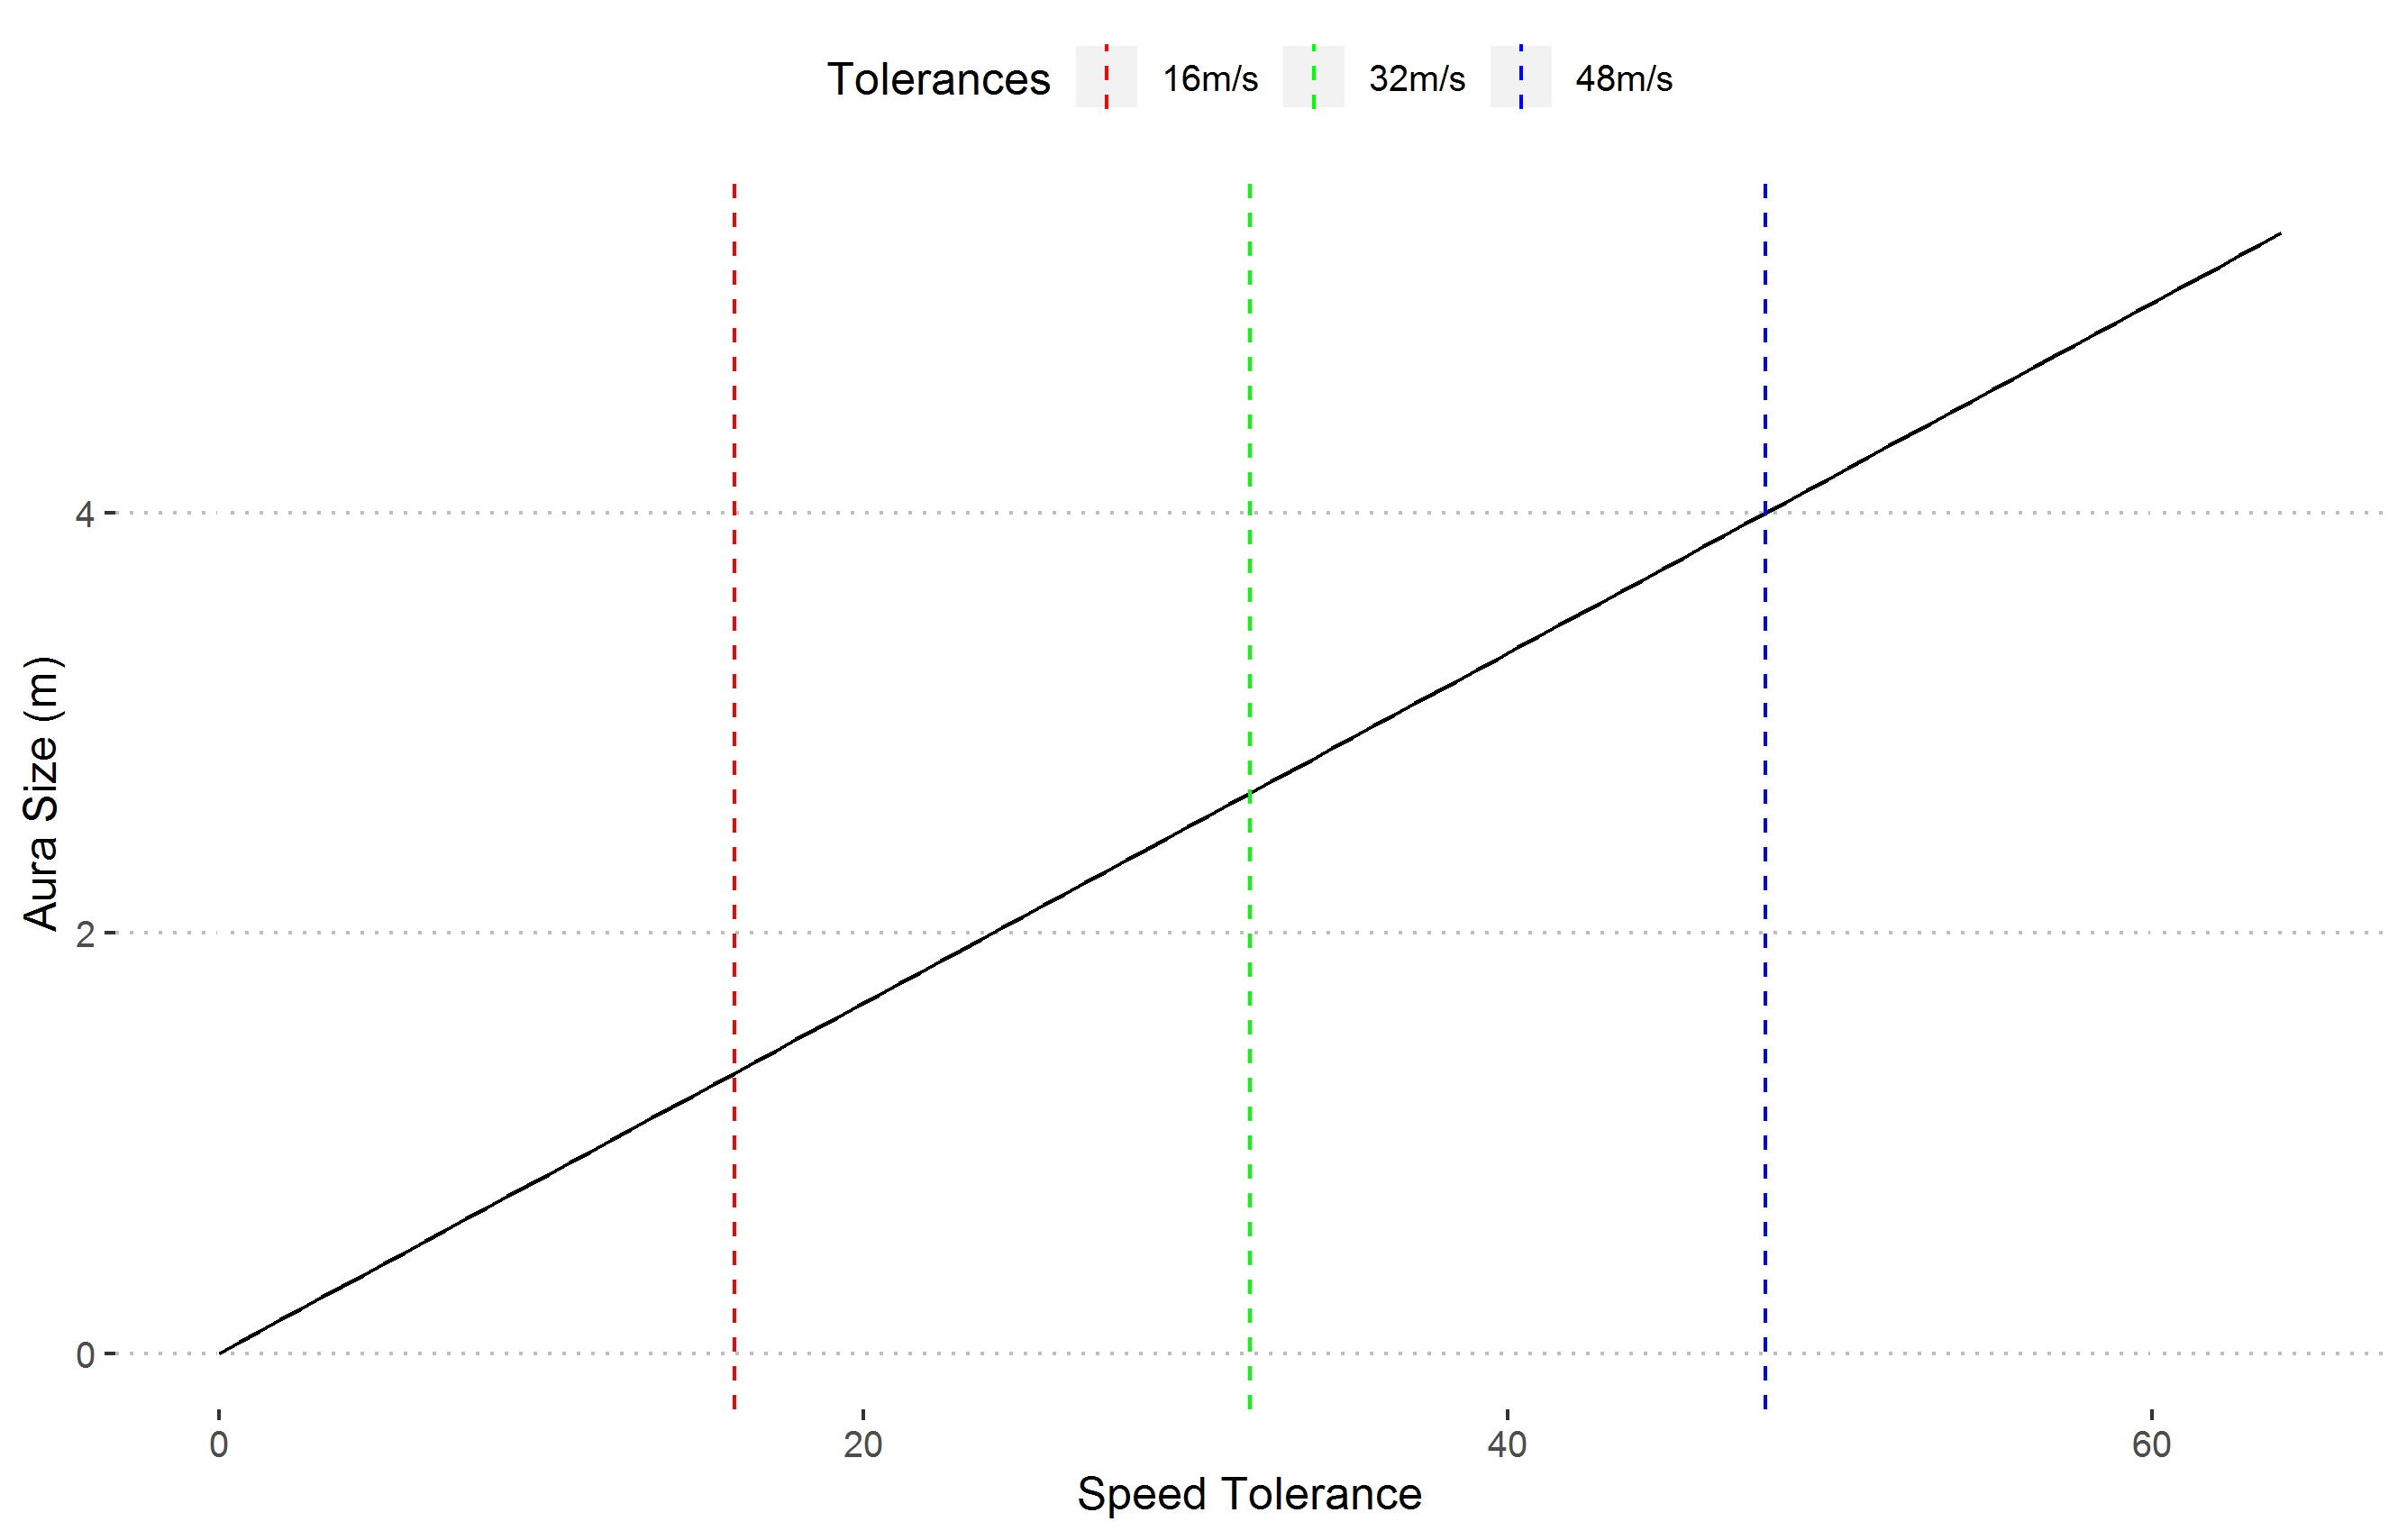
\includegraphics[width=\textwidth]{SpeedAuraSizes}
	\caption{Size of aura vs. speed tolerance. The speed tolerances used are marked in dashed lines}
	\label{fig_SpeedAuraSize}
\end{figure}

Fig. \ref{fig_SpeedAuraSize} shows the size of the aura (not including the bounding sphere of the object) vs increasing speed tolerance, calculated using equation \ref{auraEquation}.
The aura size increases continuously with speed, therefore we expect late collisions to begin immediately once the the speed tolerance is exceeded. False-positives are expected due to the frame-time delay method and should increase as speed increases.

\begin{figure}
	\centering
	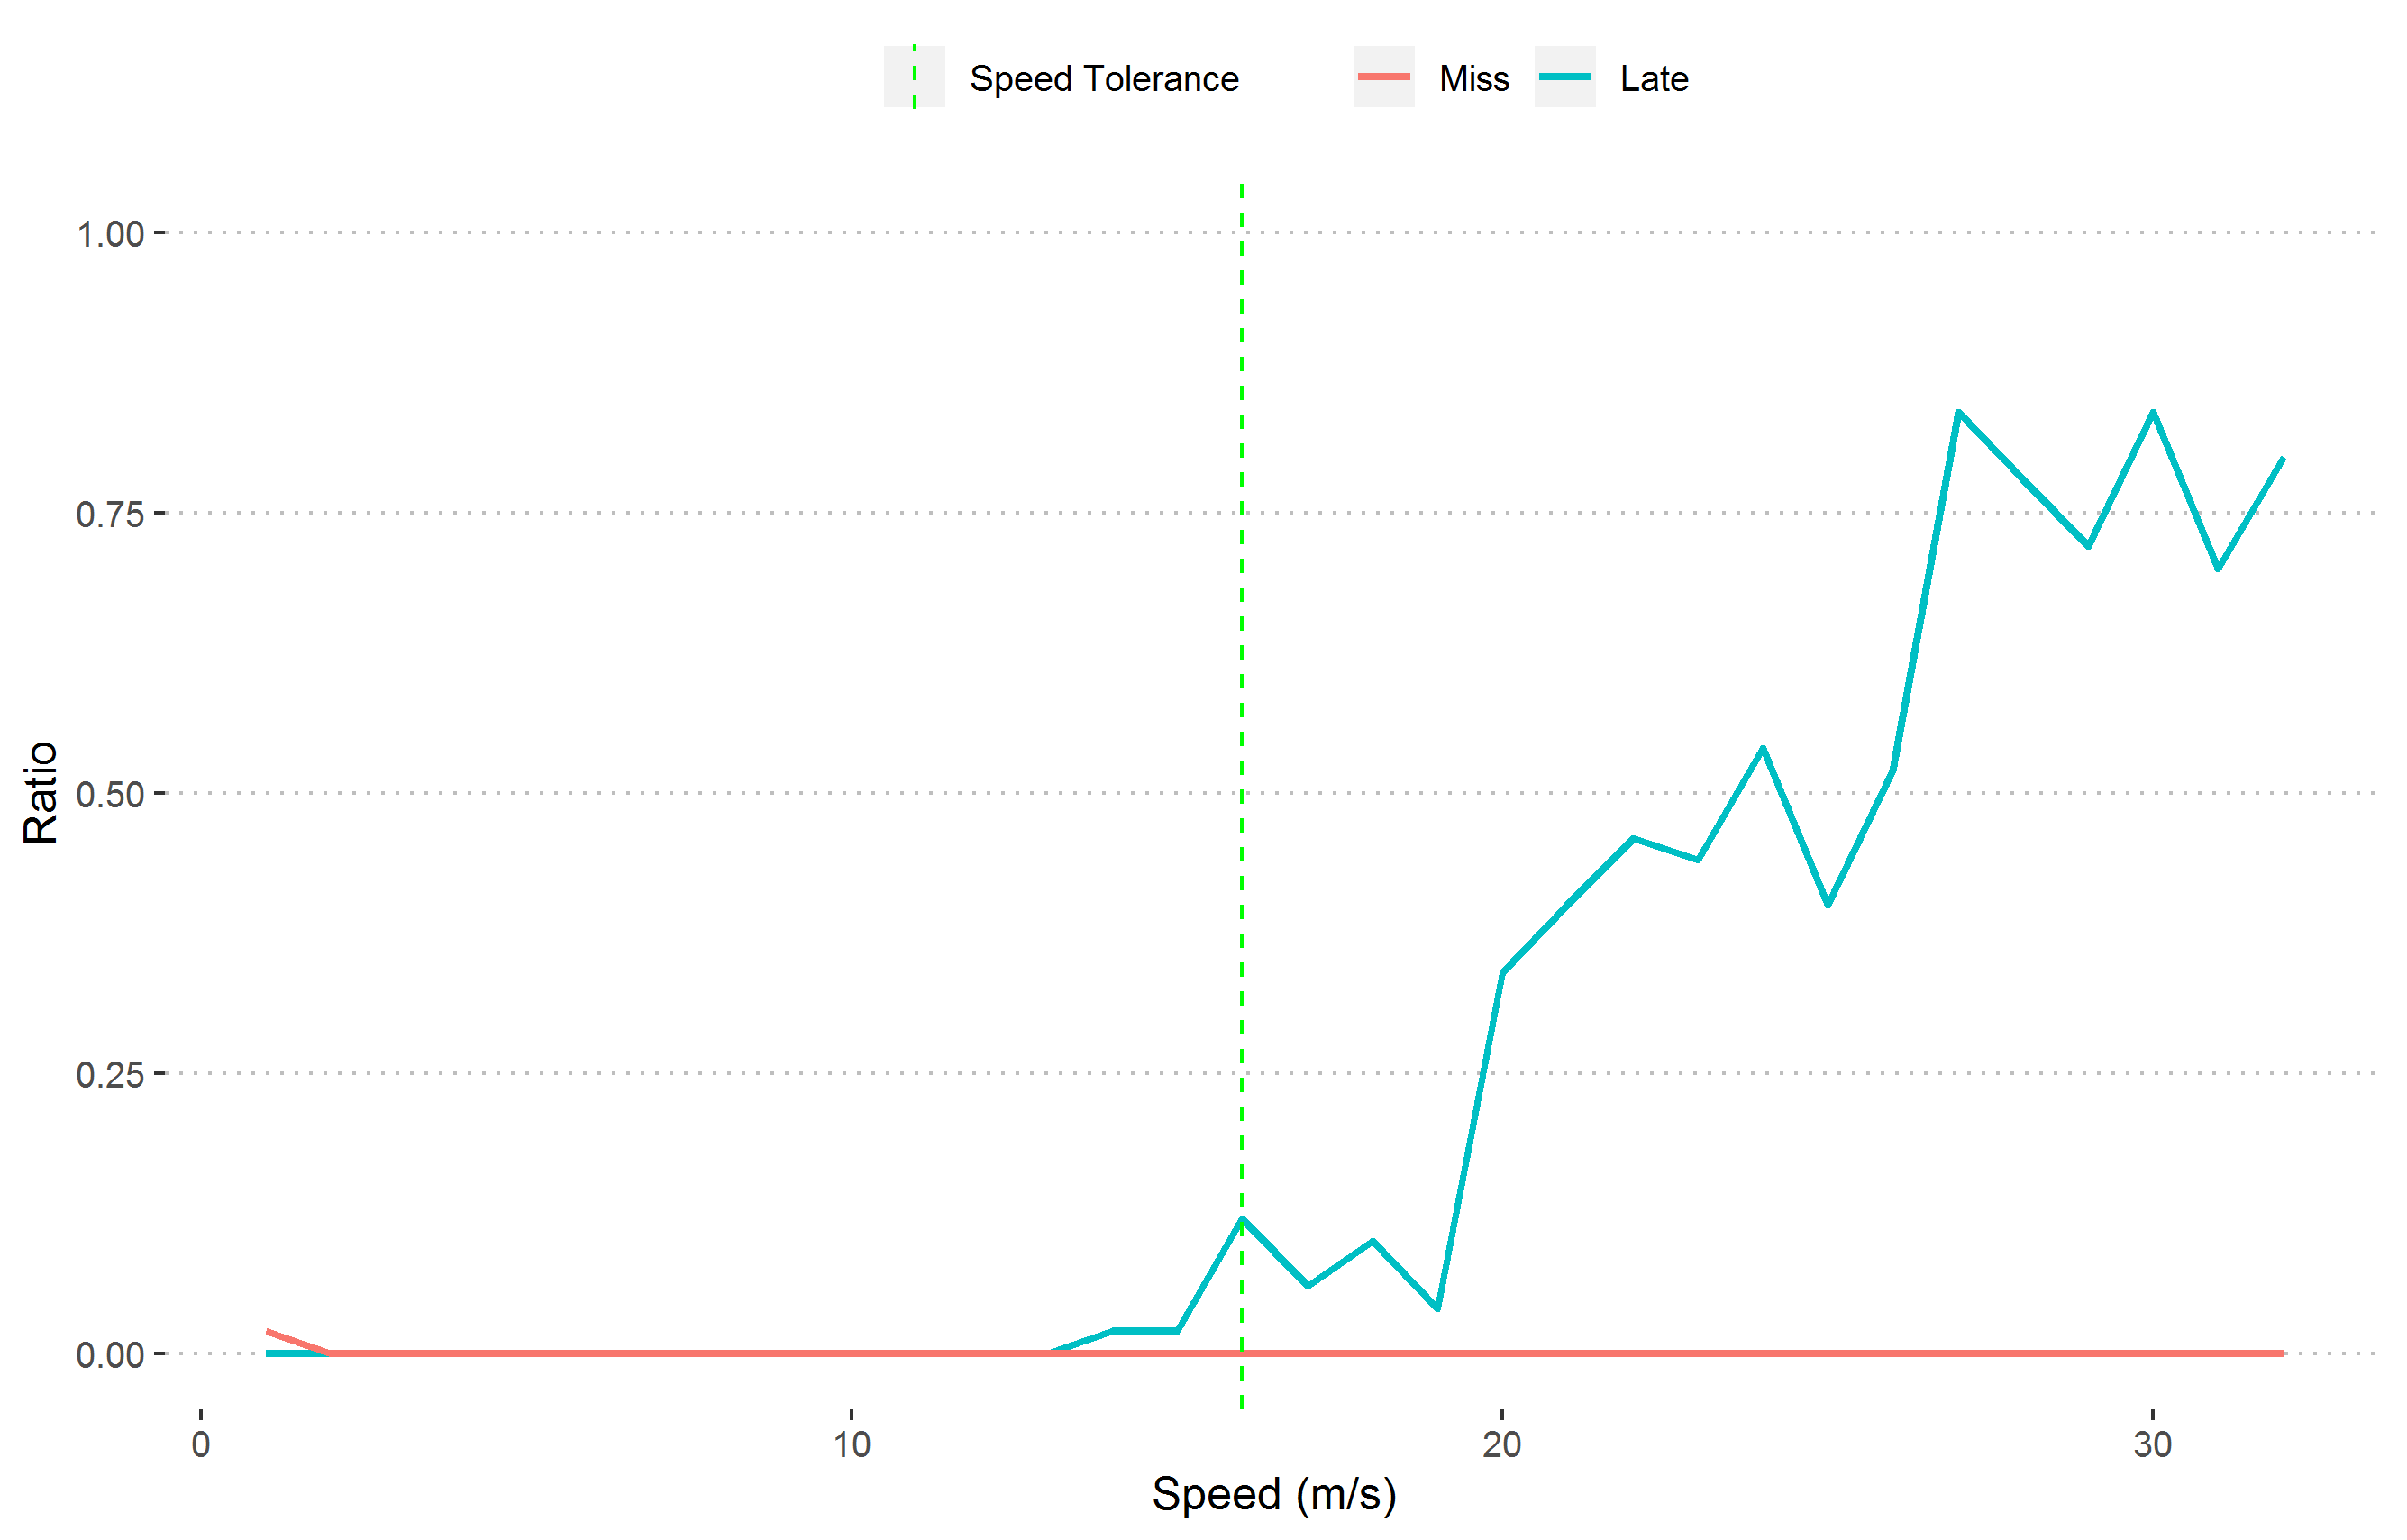
\includegraphics[width=\textwidth]{RatiosVsSpeedLow}
	\caption{Ratio of Late to Correct Collisions and Misses to Total Collision vs. Speed using a speed tolerance of $16m\mathord{\cdot}s^{-1}$. The speed tolerance is marked in a dashed green line.}
	\label{fig_RatioVsSpeedLow}
\end{figure}
\begin{figure}
	\centering
	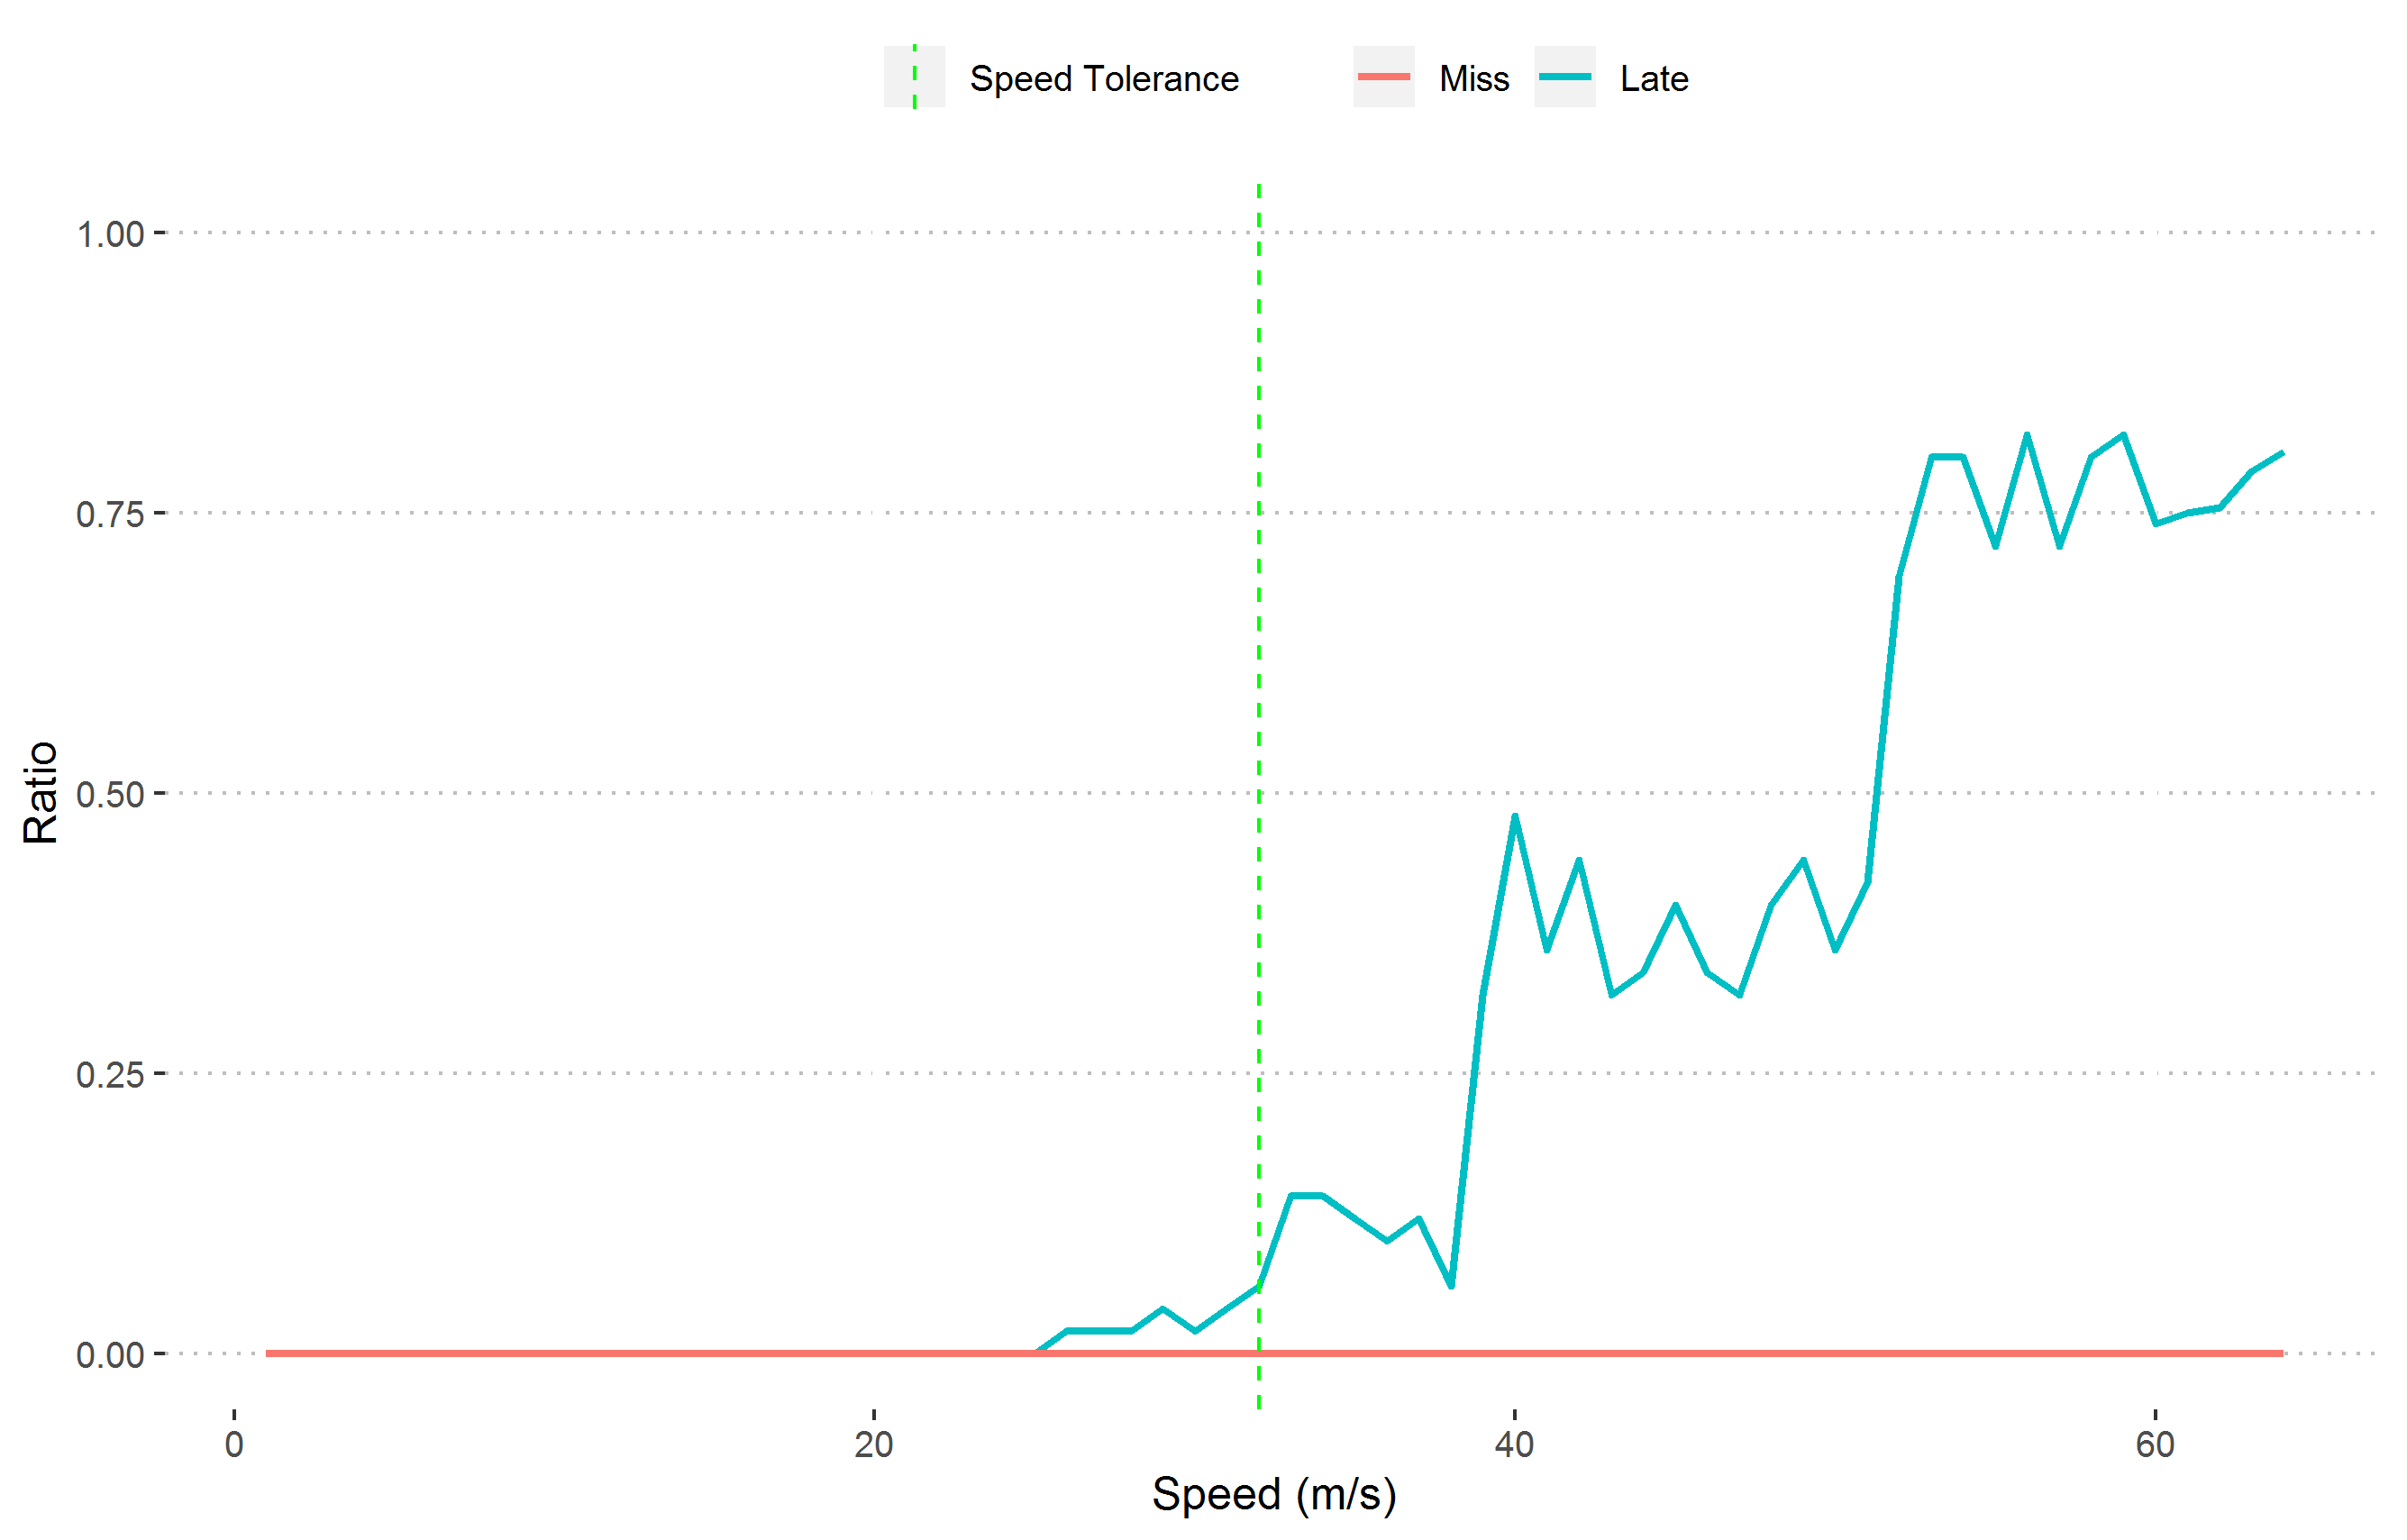
\includegraphics[width=\textwidth]{RatiosVsSpeedMid}
	\caption{Ratio of Late to Correct Collisions and Misses to Total Collision vs. Speed using a speed tolerance of $32m\mathord{\cdot}s^{-1}$. The speed tolerance is marked in a dashed green line.}
	\label{fig_RatioVsSpeedMid}
\end{figure}
\begin{figure}
	\centering
	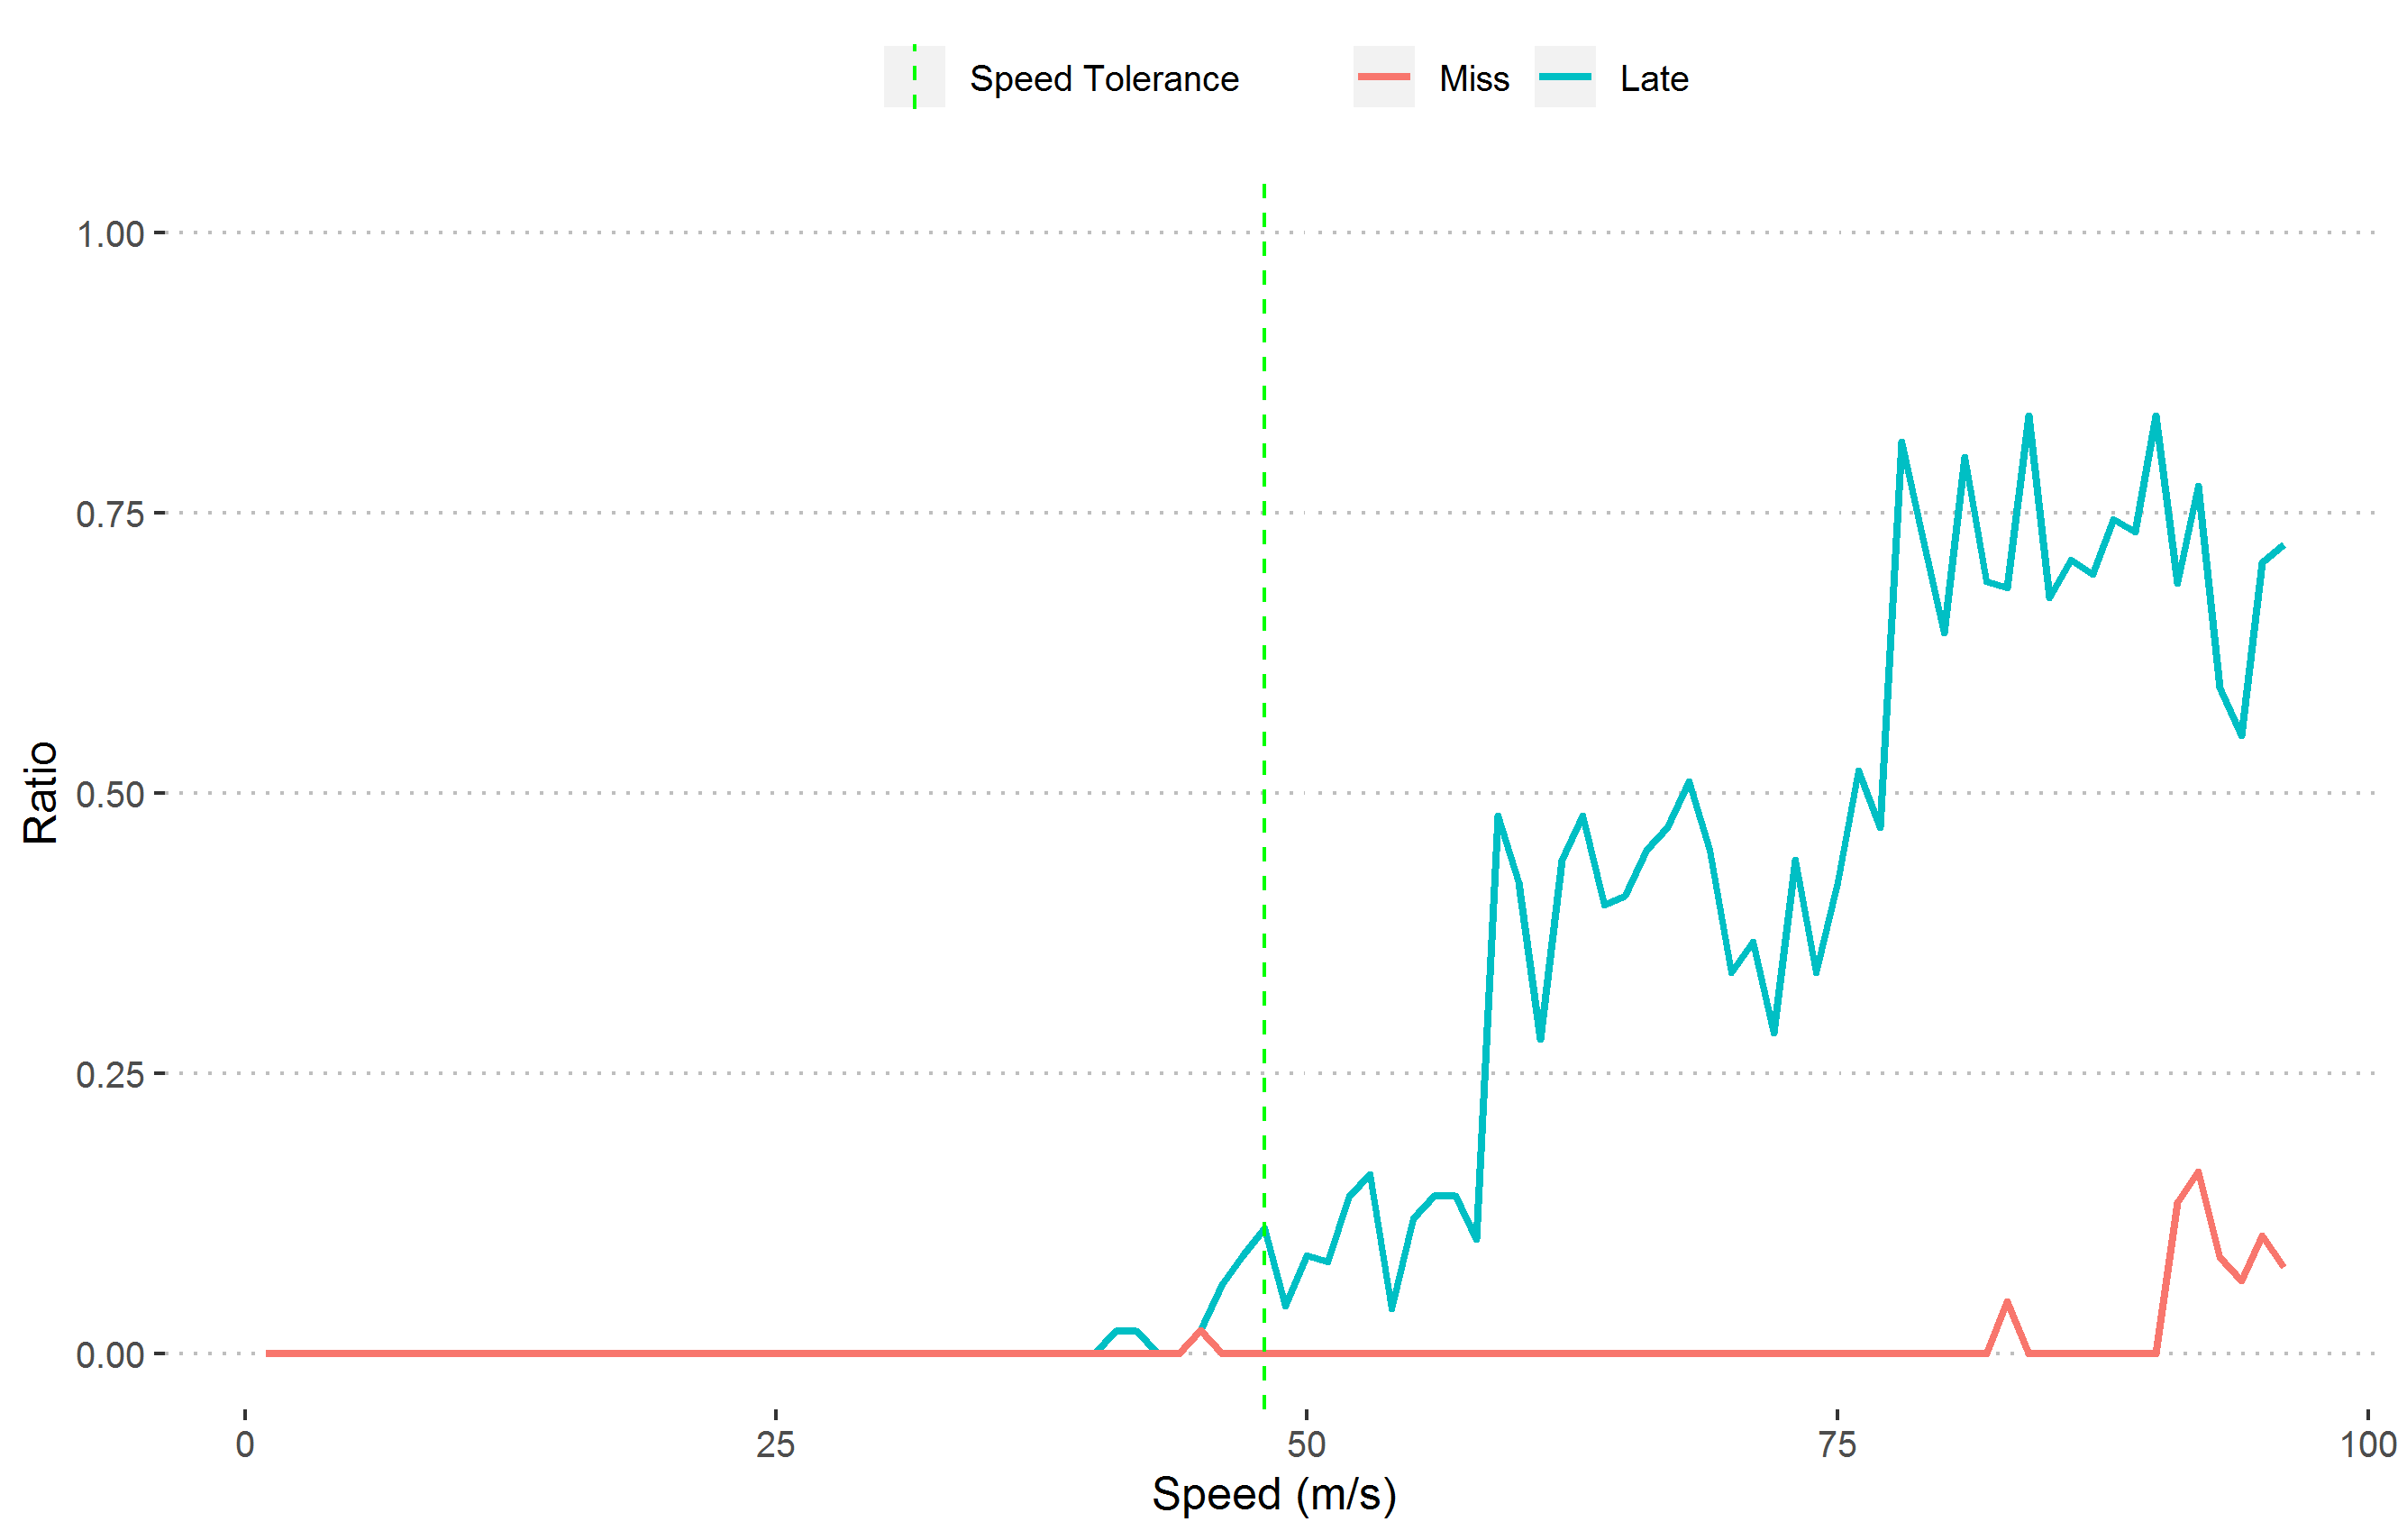
\includegraphics[width=\textwidth]{RatiosVsSpeedHigh}
	\caption{Ratio of Late to Correct Collisions and Misses to Total Collision vs. Speed using a speed tolerance of $48m\mathord{\cdot}s^{-1}$. The speed tolerance is marked in a dashed green line.}
	\label{fig_RatioVsSpeedHigh}
\end{figure}

\begin{figure}
	\centering
	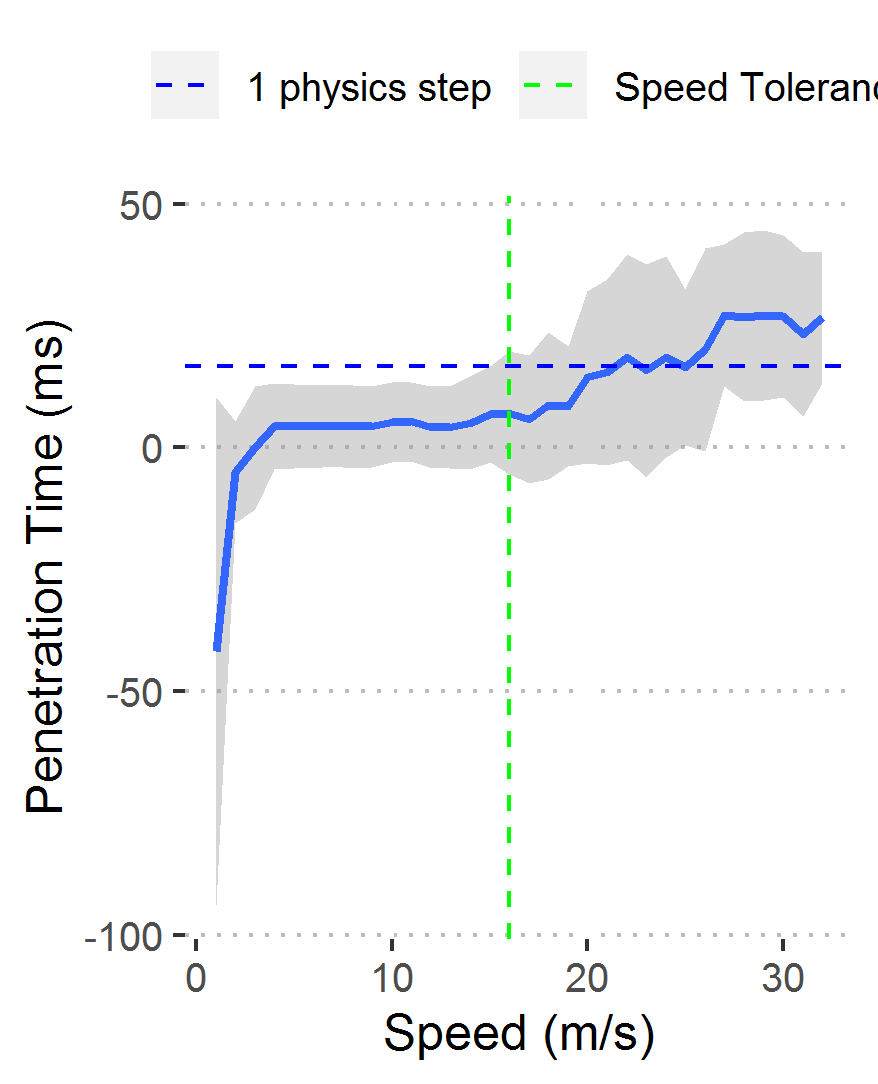
\includegraphics[width=\textwidth]{MeanPenVsSpeedLow}
	\caption{Mean penetration time of objects with $+/-2$ standard deviations with varying speed using a speed tolerance of $16m\mathord{\cdot}s^{-1}$. The maximum expected penetration time of 1 physics step is marked with a dashed blue line. The speed tolerance is marked in a dashed green line.}
	\label{fig_CollisionsPenVsSpeedLow}
\end{figure}
\begin{figure}
	\centering
	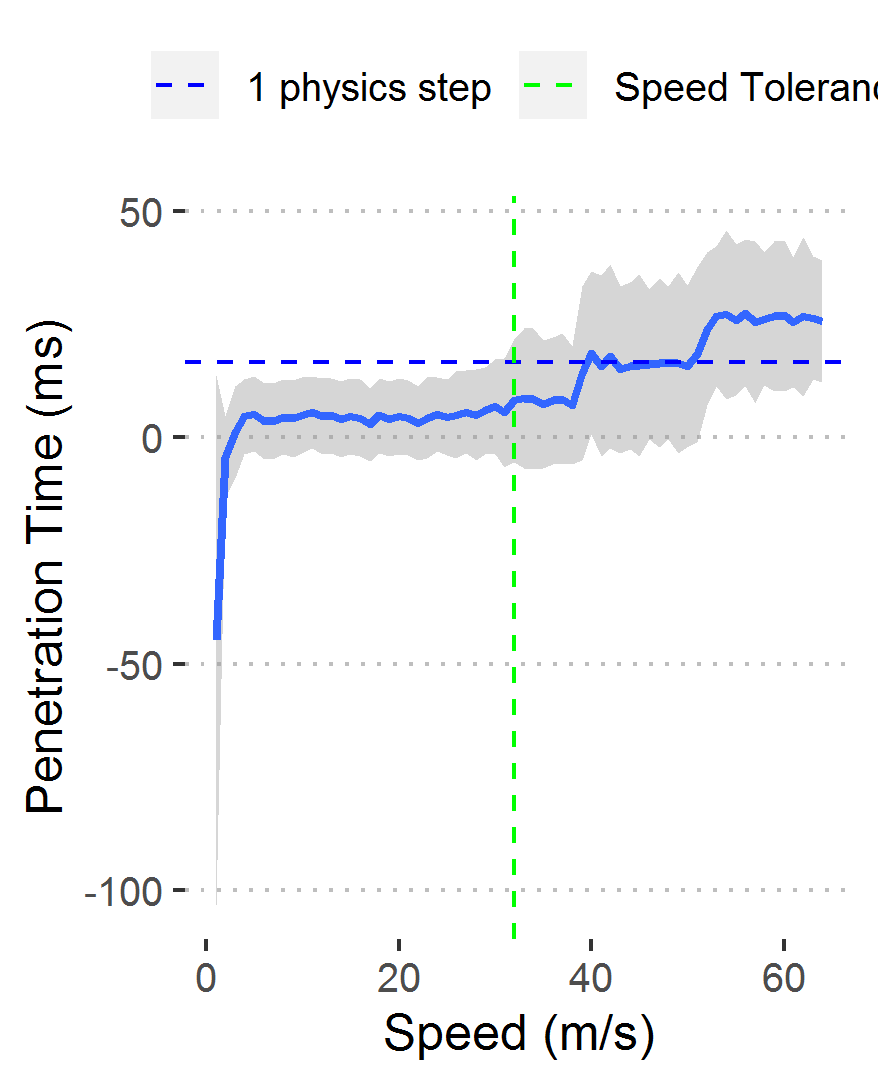
\includegraphics[width=\textwidth]{MeanPenVsSpeedMid}
	\caption{Mean penetration time of objects with $+/-2$ standard deviations with varying speed using a speed tolerance of $32m\mathord{\cdot}s^{-1}$. The maximum expected penetration time of 1 physics step is marked with a dashed blue line. The speed tolerance is marked in a dashed green line.}
	\label{fig_CollisionsPenVsSpeedMid}
\end{figure}
\begin{figure}
	\centering
	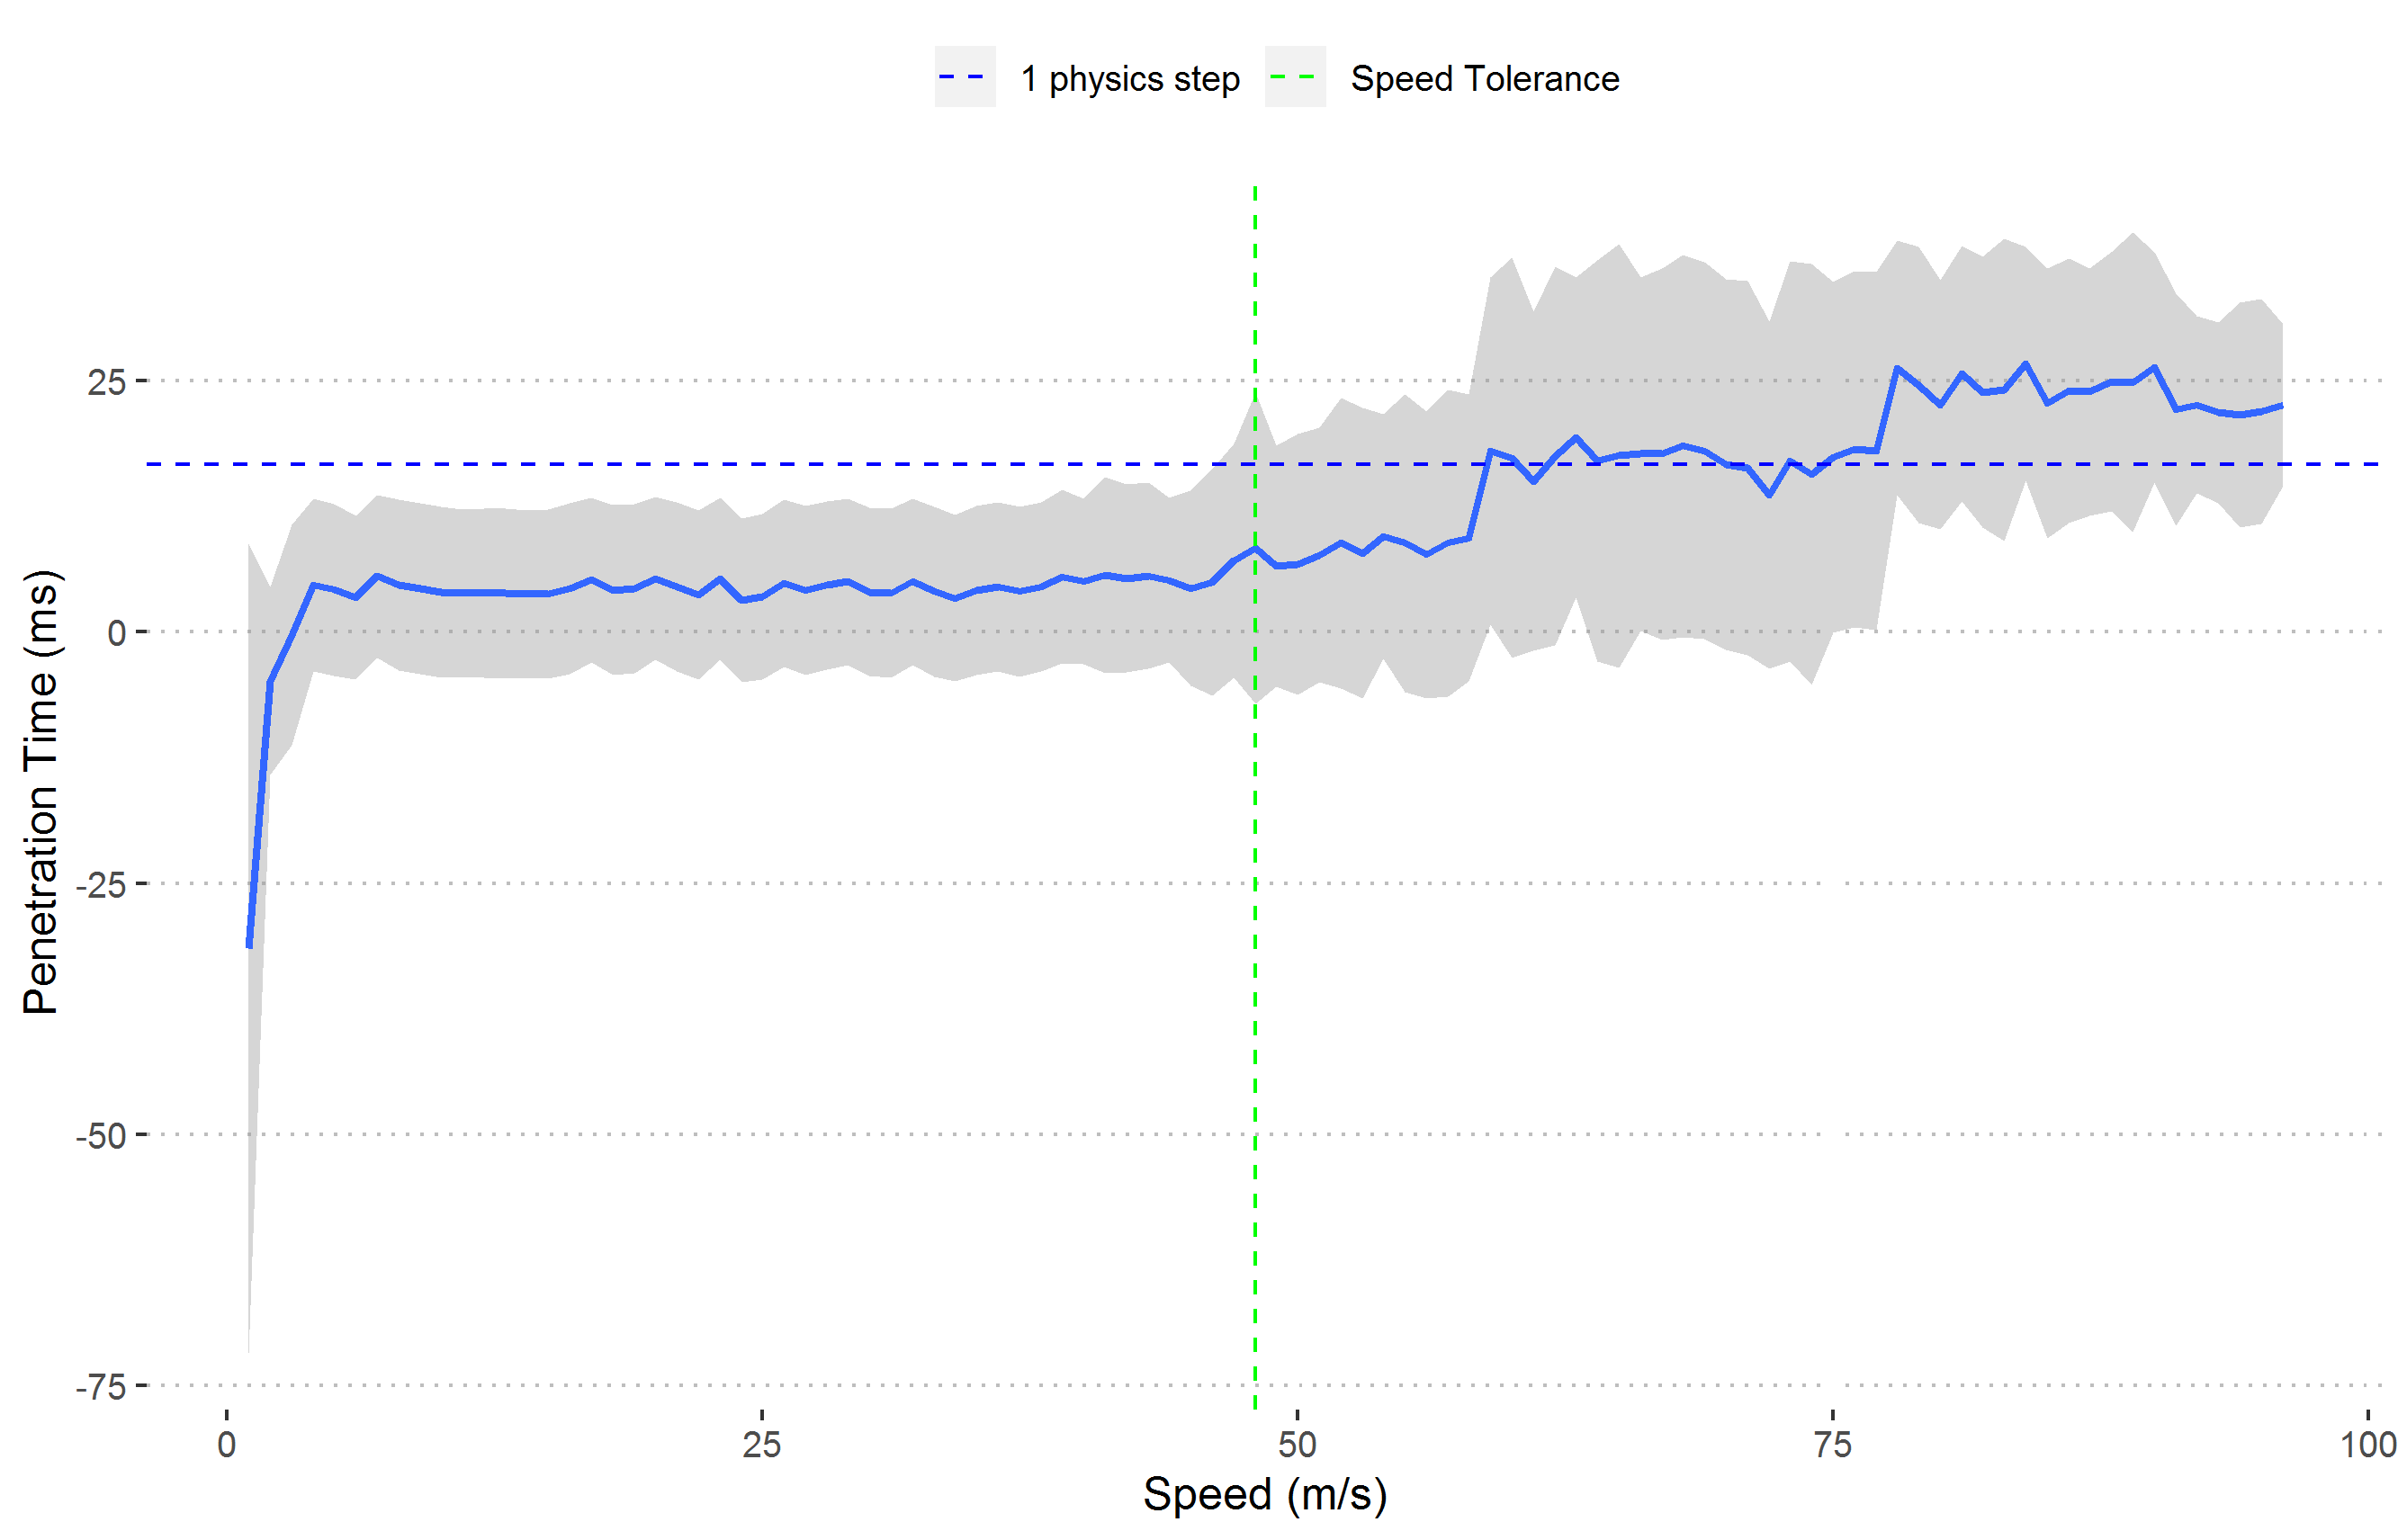
\includegraphics[width=\textwidth]{MeanPenVsSpeedHigh}
	\caption{Mean penetration time of objects with $+/-2$ standard deviations with varying speed using a speed tolerance of $48m\mathord{\cdot}s^{-1}$. The maximum expected penetration time of 1 physics step is marked with a dashed blue line. The speed tolerance is marked in a dashed green line.}
	\label{fig_CollisionsPenVsSpeedHigh}
\end{figure}
	%\label{fig_CollisionsPenVsSpeed}
%\begin{figure}
%	\centering
%	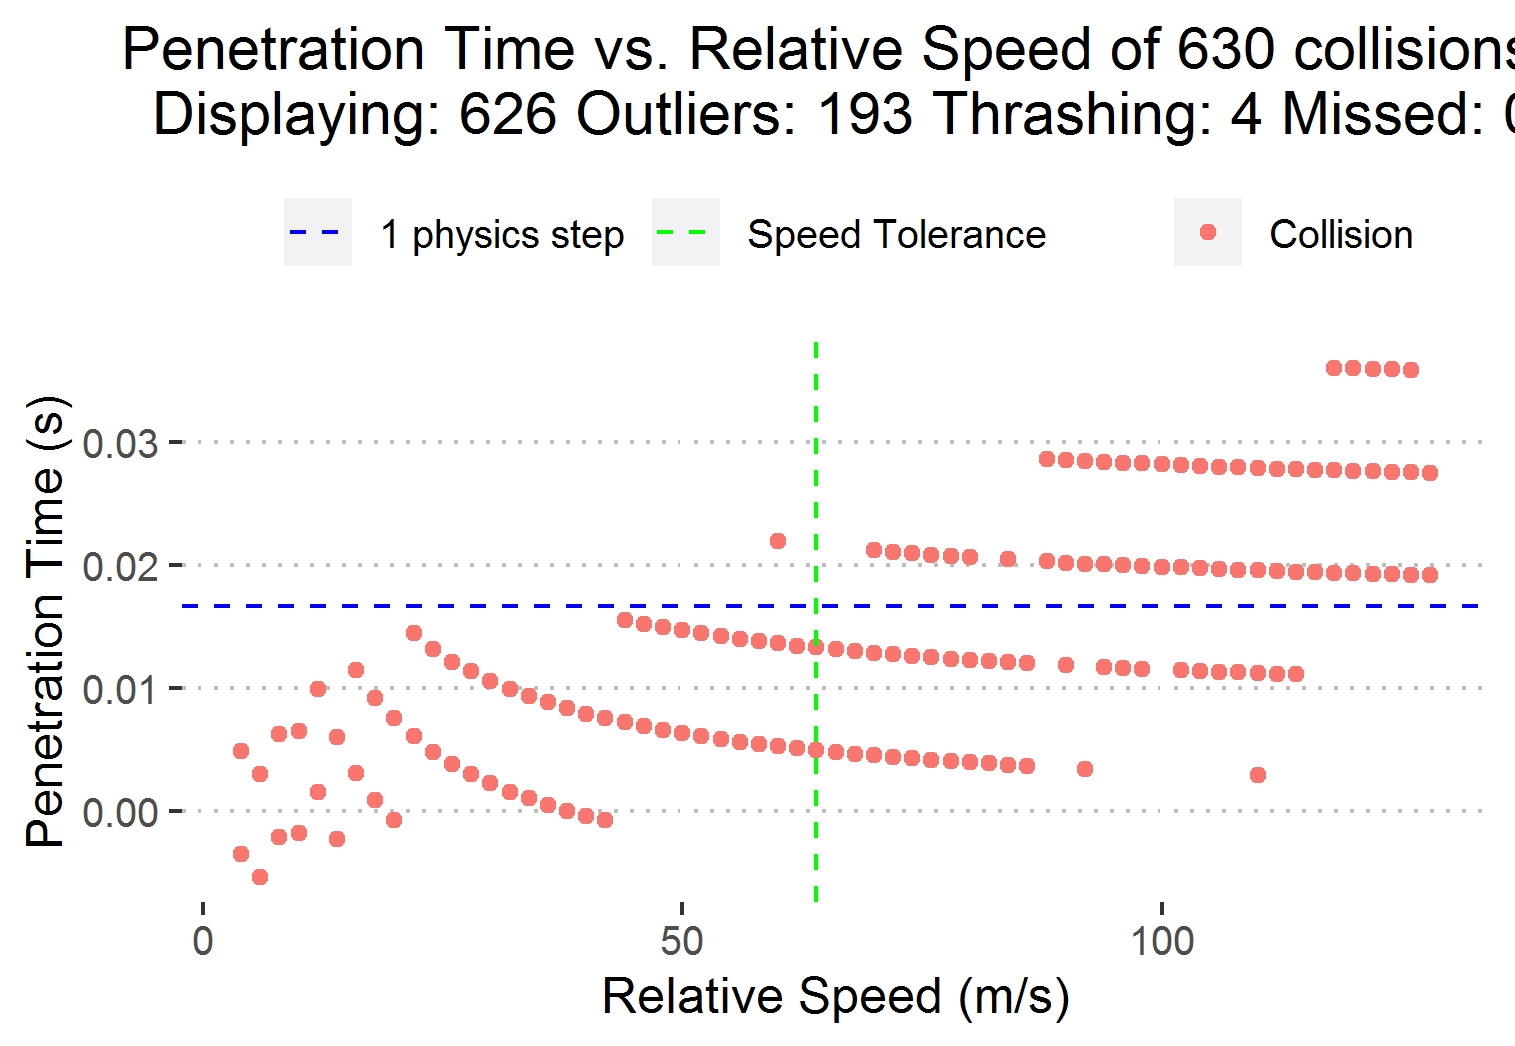
\includegraphics[width=\textwidth]{CollisionsPenVsSpeed}
%	\caption{Penetration time of objects with varying relative speed. Each red point represents one or more collisions. The maximum expected penetration time of 1 physics steps is marked with a dashed blue line. The speed tolerance is marked in a dashed green line. The number and magnitude of errors increases as relative speed increases beyond the tolerance.}
%	\label{fig_CollisionsPenVsSpeed}
%\end{figure}
%
%\begin{figure}
%\centering
%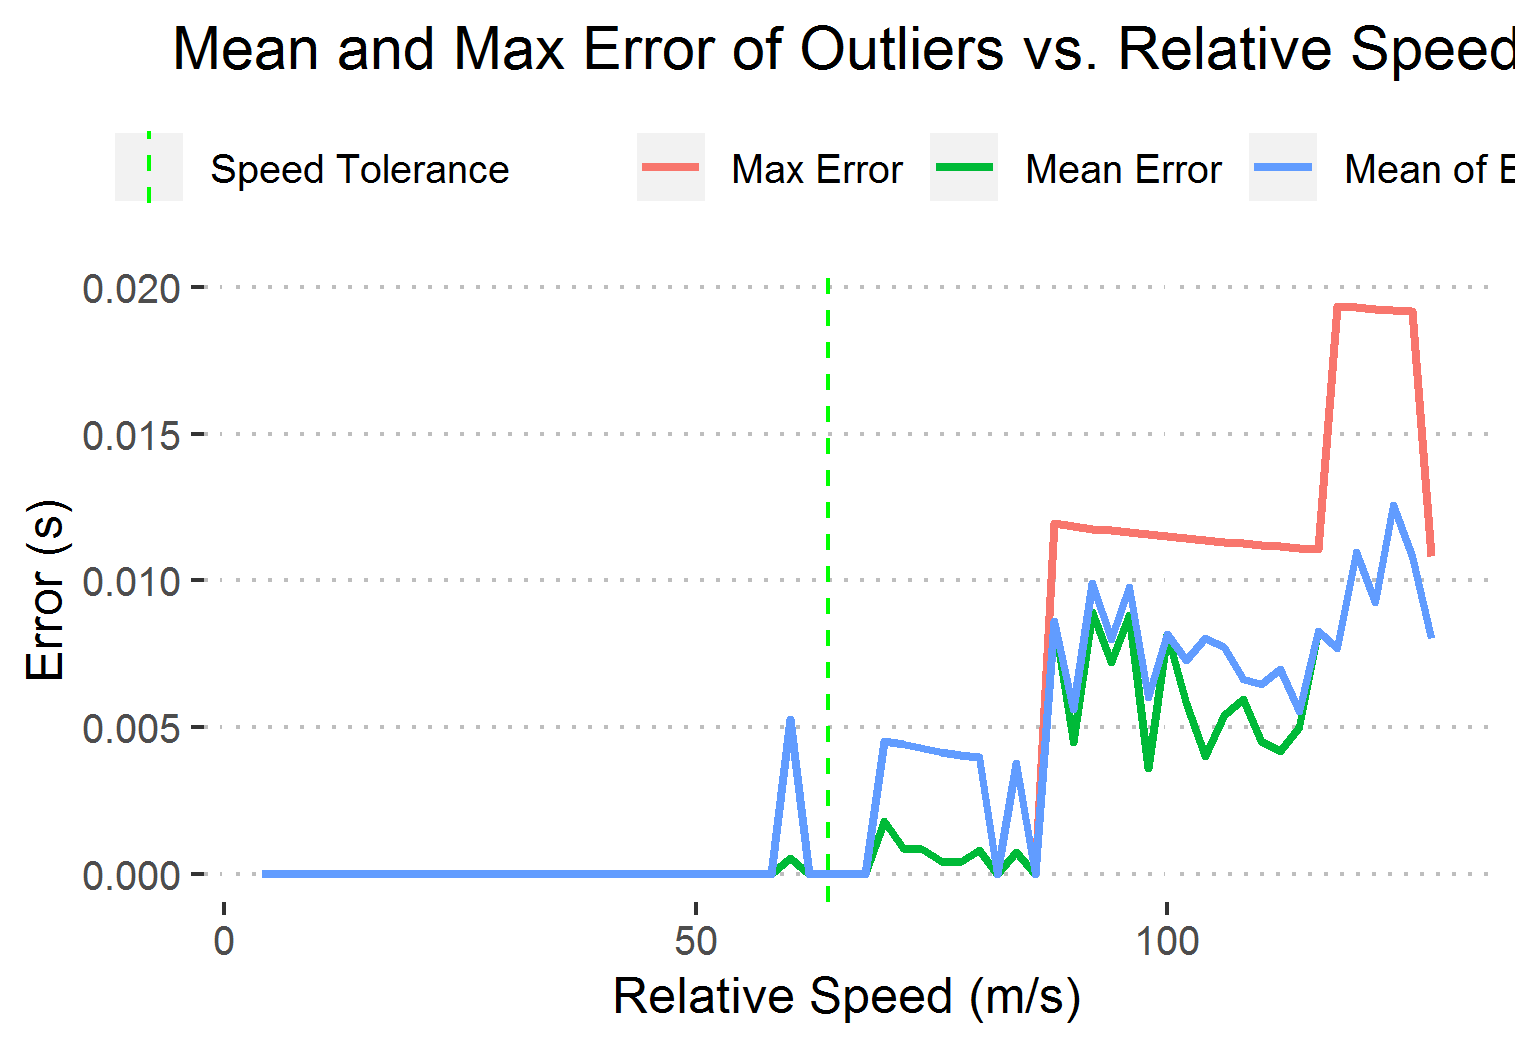
\includegraphics[width=\textwidth]{MeanMaxErrorVsSpeed}
%\caption{The mean and max of collision errors with varying relative speed}
%\label{fig_MeanMaxErrorVsSpeed}
%\end{figure}
%
%\begin{figure}
%\centering
%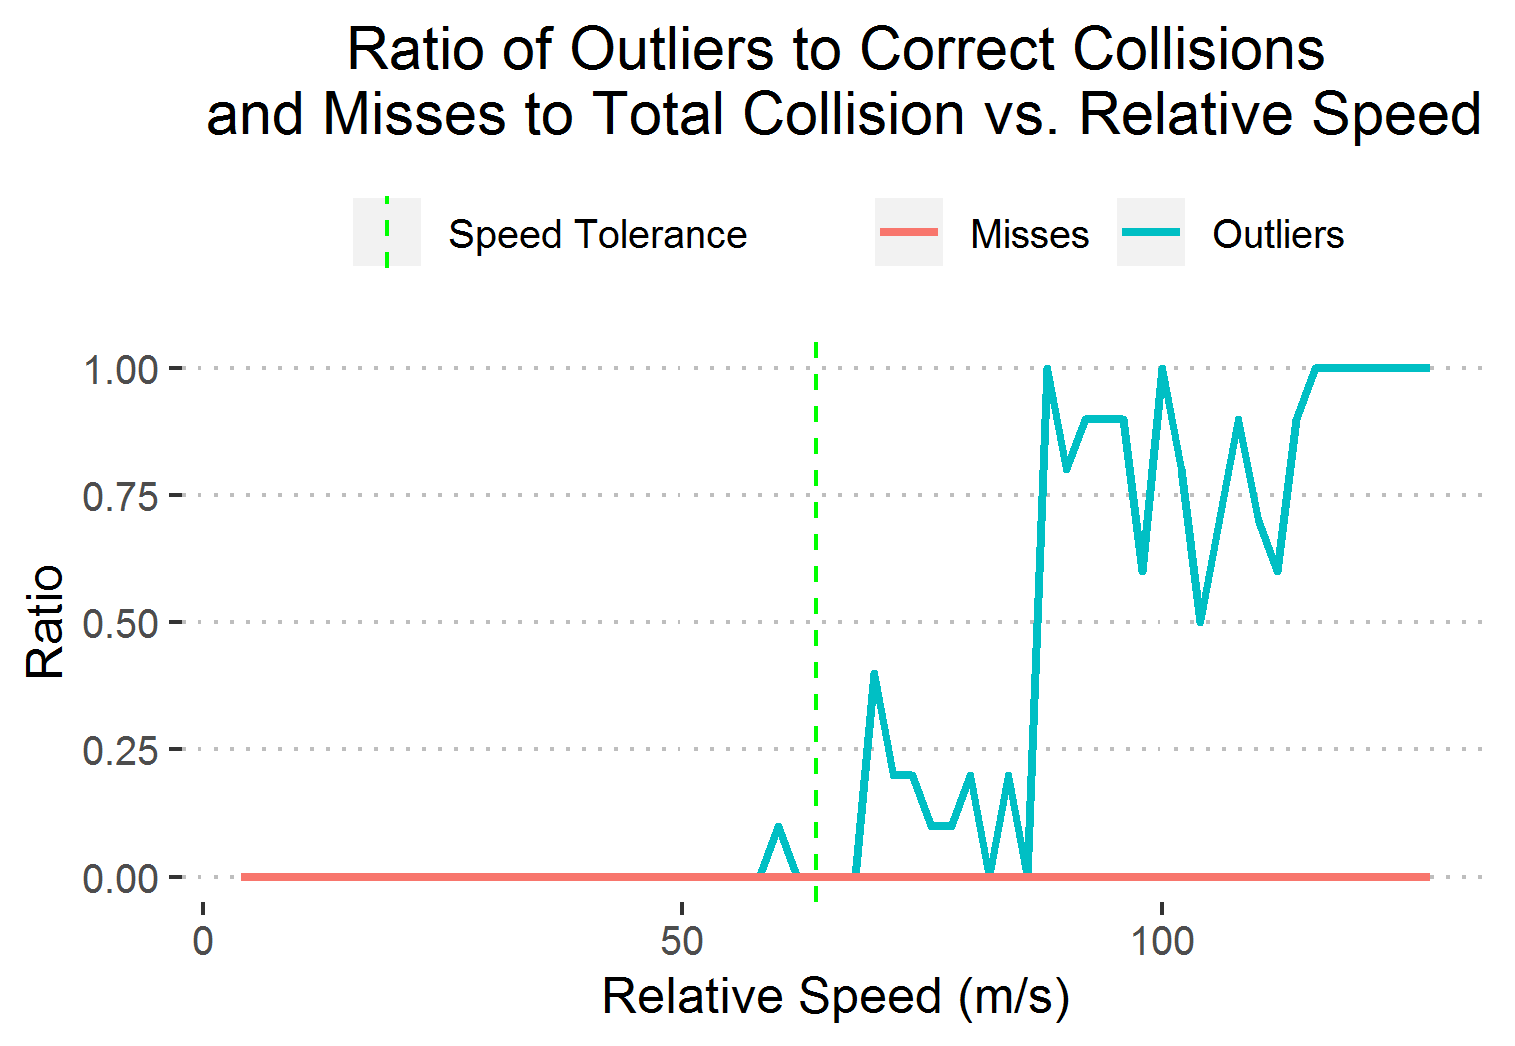
\includegraphics[width=\textwidth]{RatiosVsSpeed}
%\caption{The ratios of erroneous collisions to correct collisions and missed collisions to total collisions with varying relative speed}
%\label{fig_RatiosVsSpeed}
%\end{figure}

\subsubsection{Varying Latency}

In this experiment the latency between the two servers was varied from $0ms$ to double the following tolerances: $2ms$; $8ms$ and $16ms$ in increments of $0.05ms$, $0.25ms$ and $1ms$ respectively. The latency used is the target latency, in reality the latency will never exactly be equal to $0ms$.

\begin{figure}
	\centering
	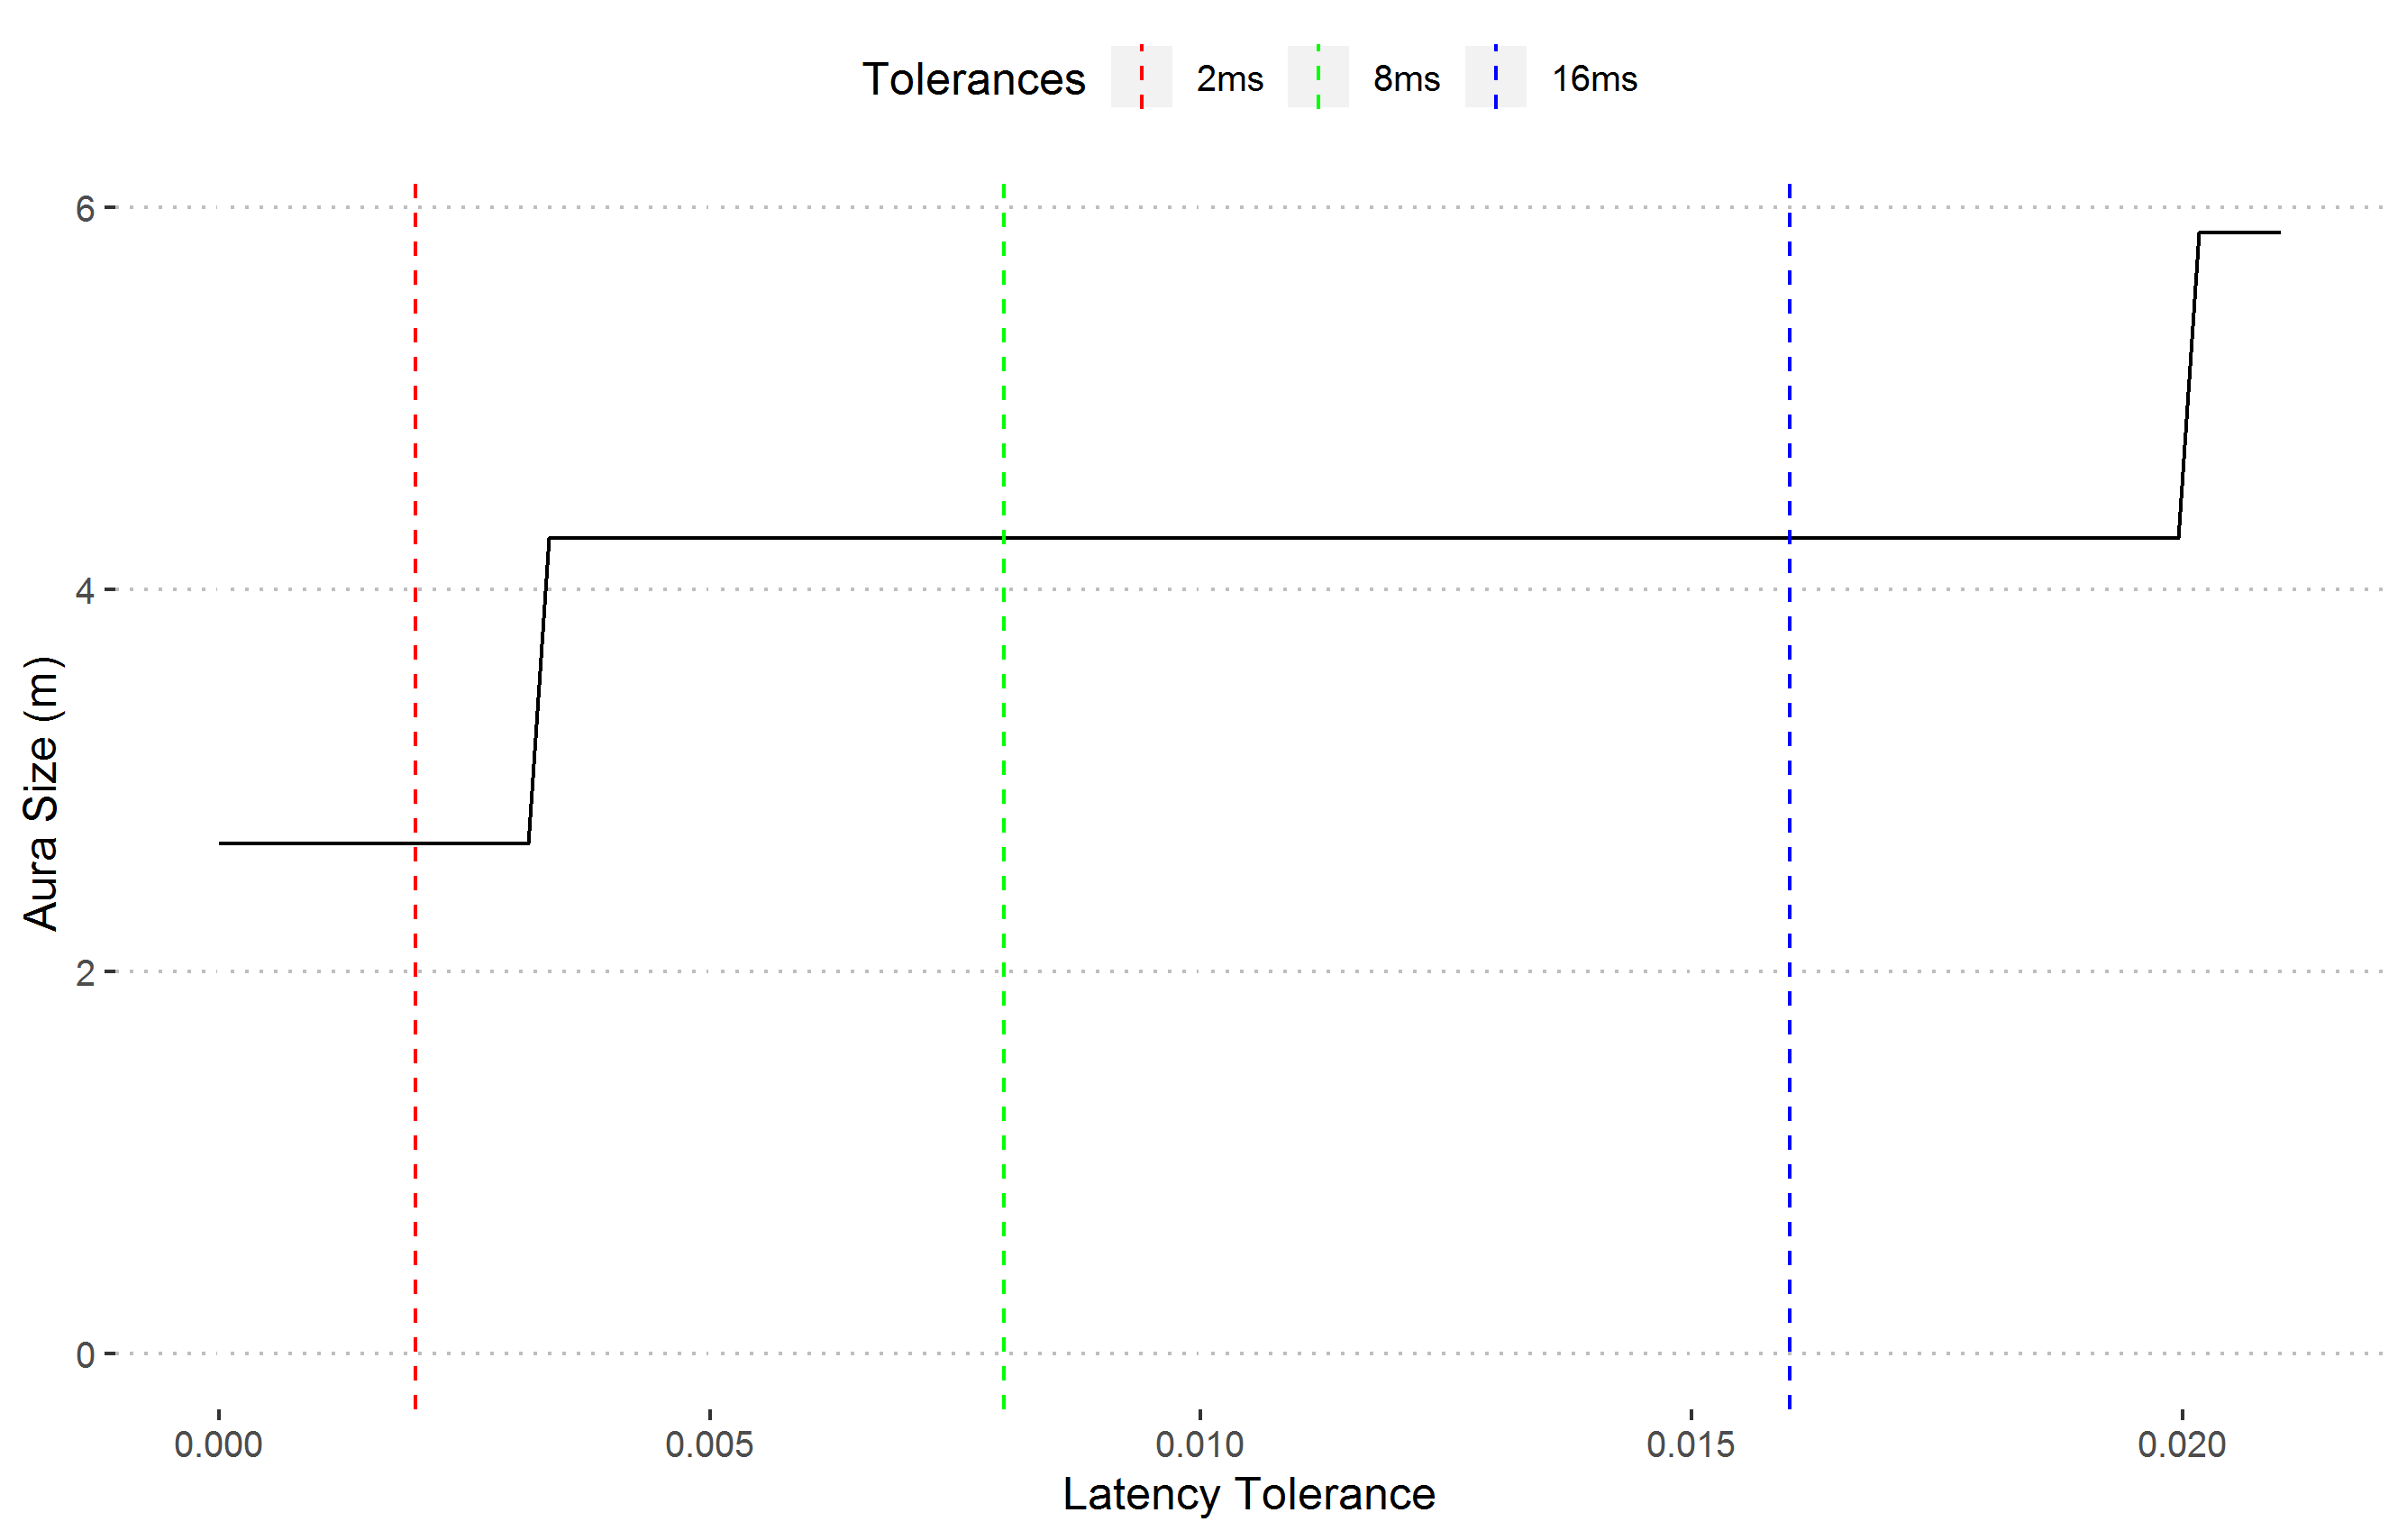
\includegraphics[width=\textwidth]{LatencyAuraSizes}
	\caption{Size of aura vs. latency tolerance. The latency tolerances used are marked in dashed lines}
	\label{fig_LatencyAuraSize}
\end{figure}

Fig. \ref{fig_LatencyAuraSize} shows the size of the aura (not including the bounding sphere of the object) vs increasing latency tolerance, calculated using equation \ref{auraEquation}. The aura size increases discretely with latency tolerance, for example tolerance values from $4ms$ to $20ms$ result in the same aura size. Late collisions are expected to occur only once the actual latency exceeds the maximum tolerance for the current aura size. In the following experiments, this means that in the $2ms$ tolerance experiments, late collisions are not expected to occur until the actual latency exceeds $3ms$. Likewise, in the $8ms$ and $16ms$ tolerance experiments, $20ms$ actual latency is expected to be reached before late collisions begin to occur. Note that late collisions are not expected for the $8ms$ experiment, as $20ms$ latency is not reached. False-positives are expected due to the frame-time delay method and should increase as actual latency increases.

\begin{figure}
	\centering
	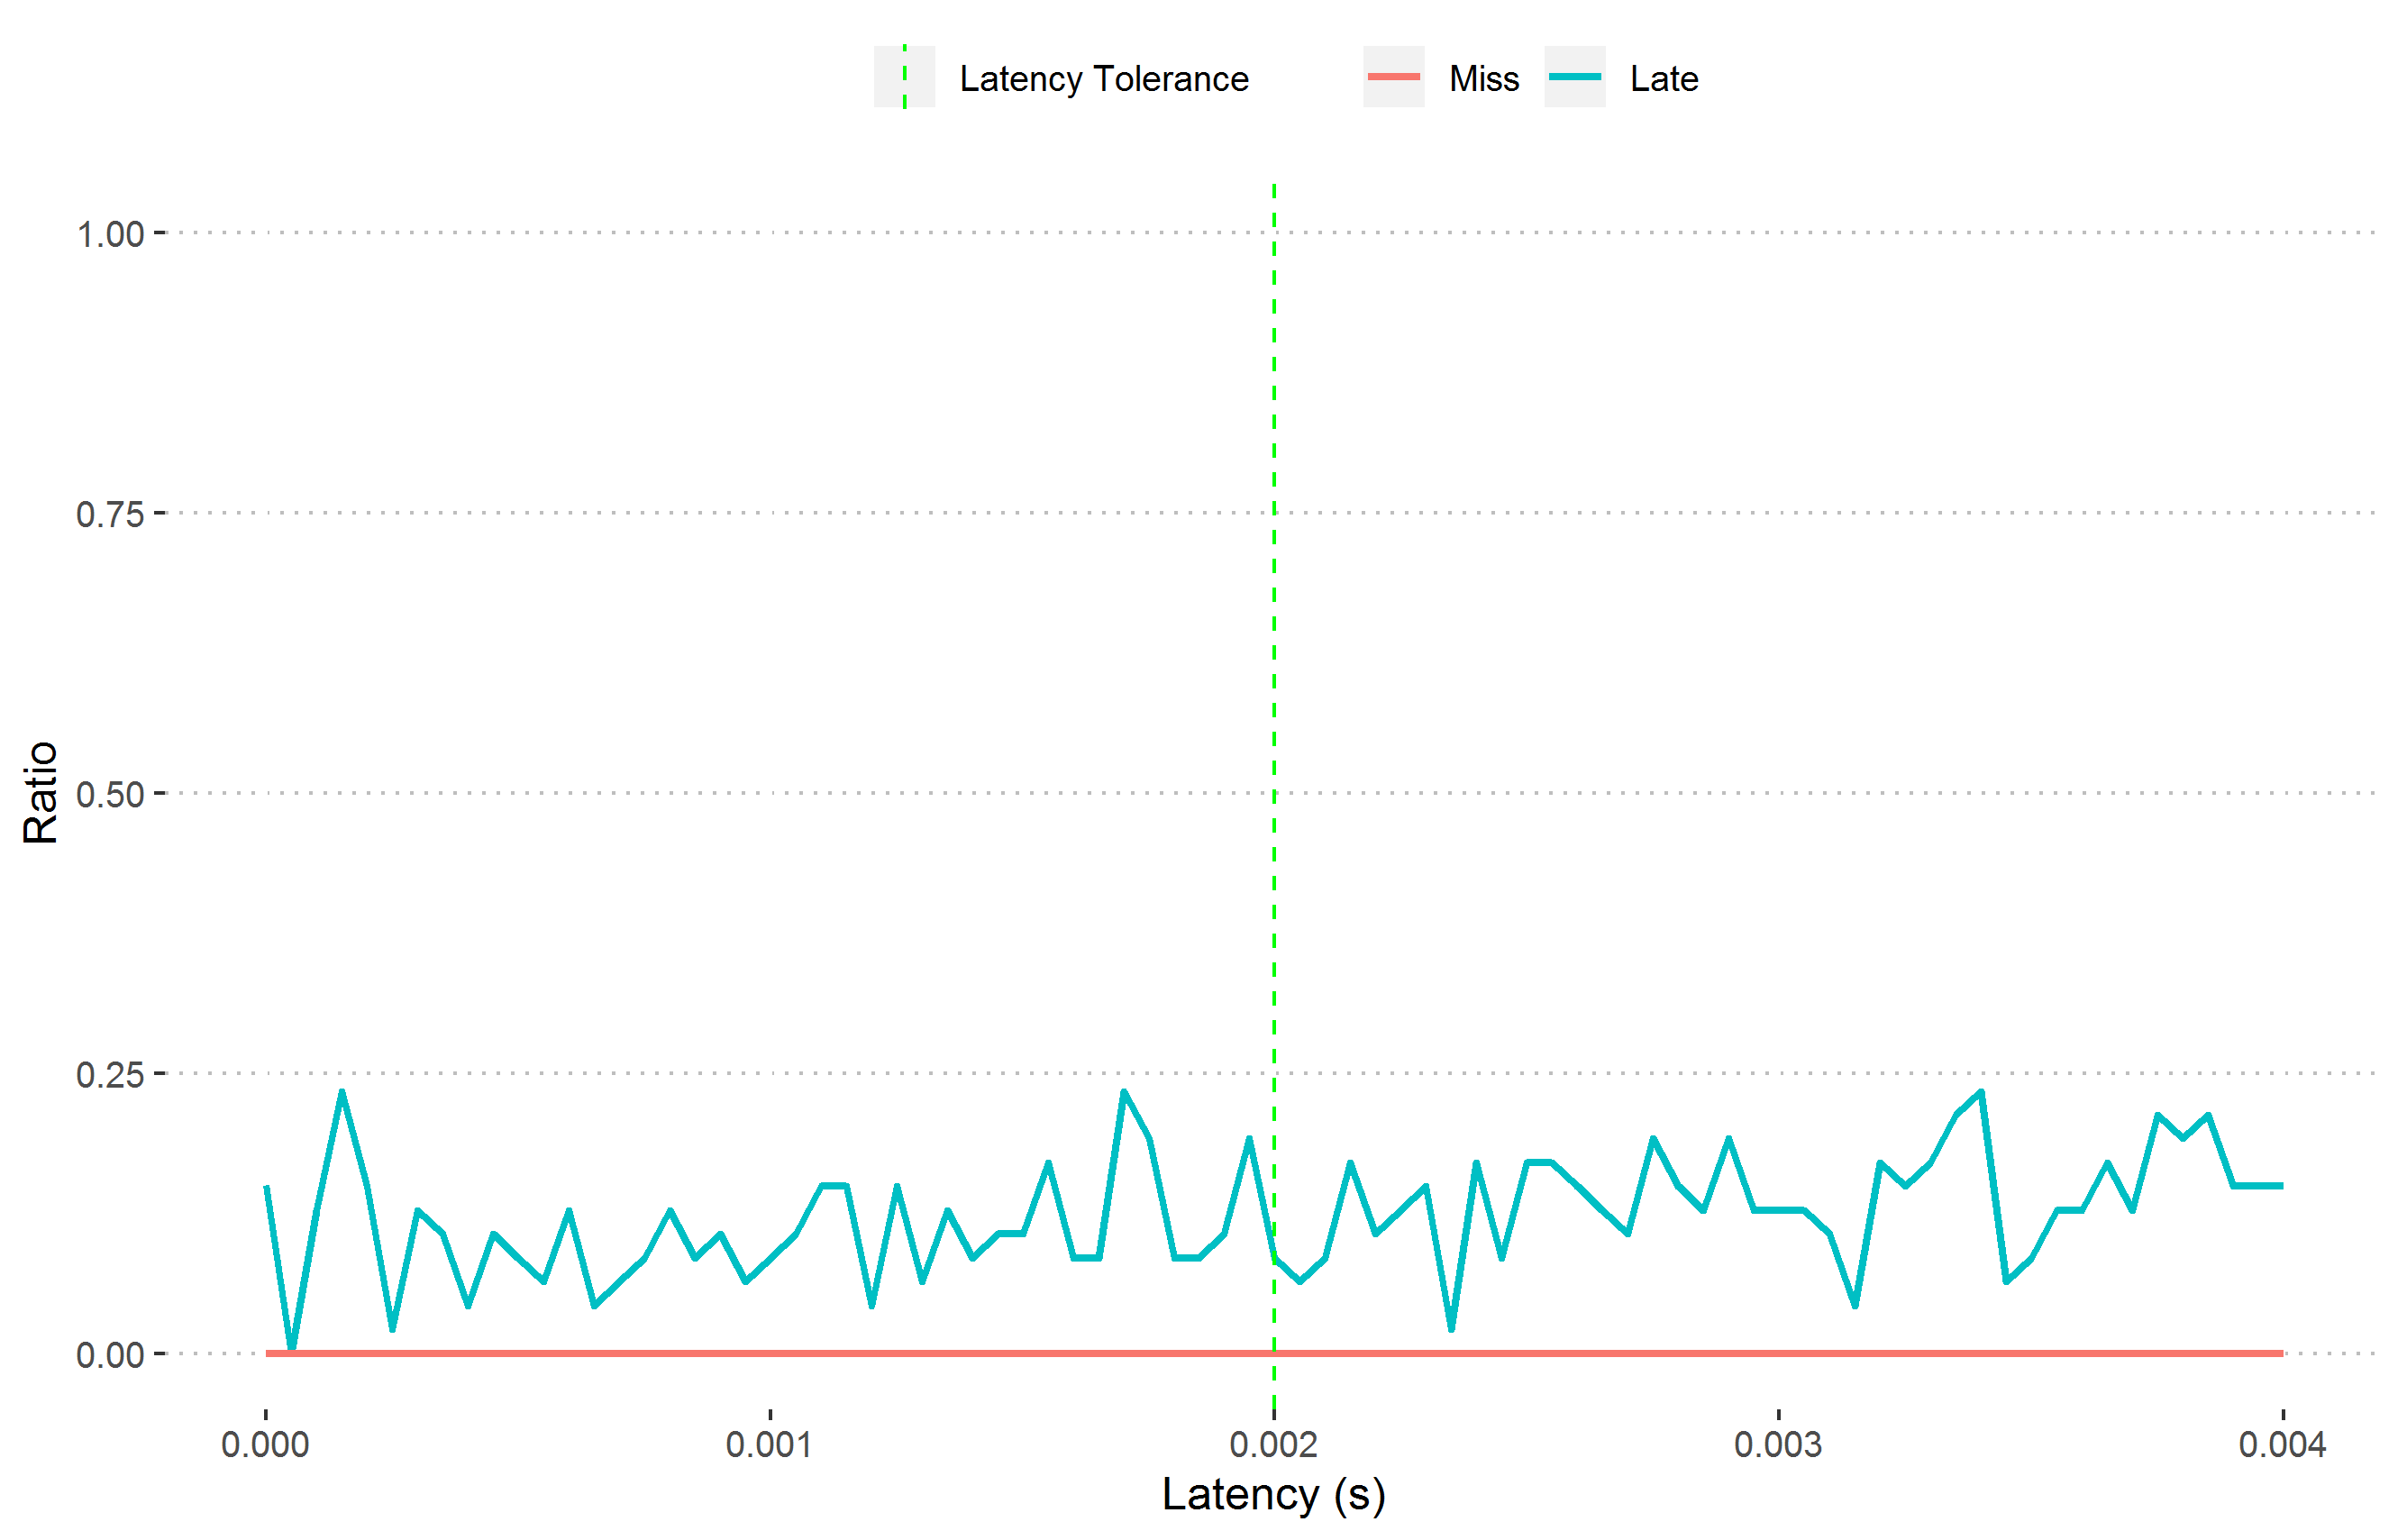
\includegraphics[width=\textwidth]{RatiosVsLatencyLow}
	\caption{Ratio of Late to Correct Collisions and Misses to Total Collision vs. Latency using a latency tolerance of $2ms$. The latency tolerance is marked in a dashed green line.}
	\label{fig_RatioVsLatencyLow}
\end{figure}
\begin{figure}
	\centering
	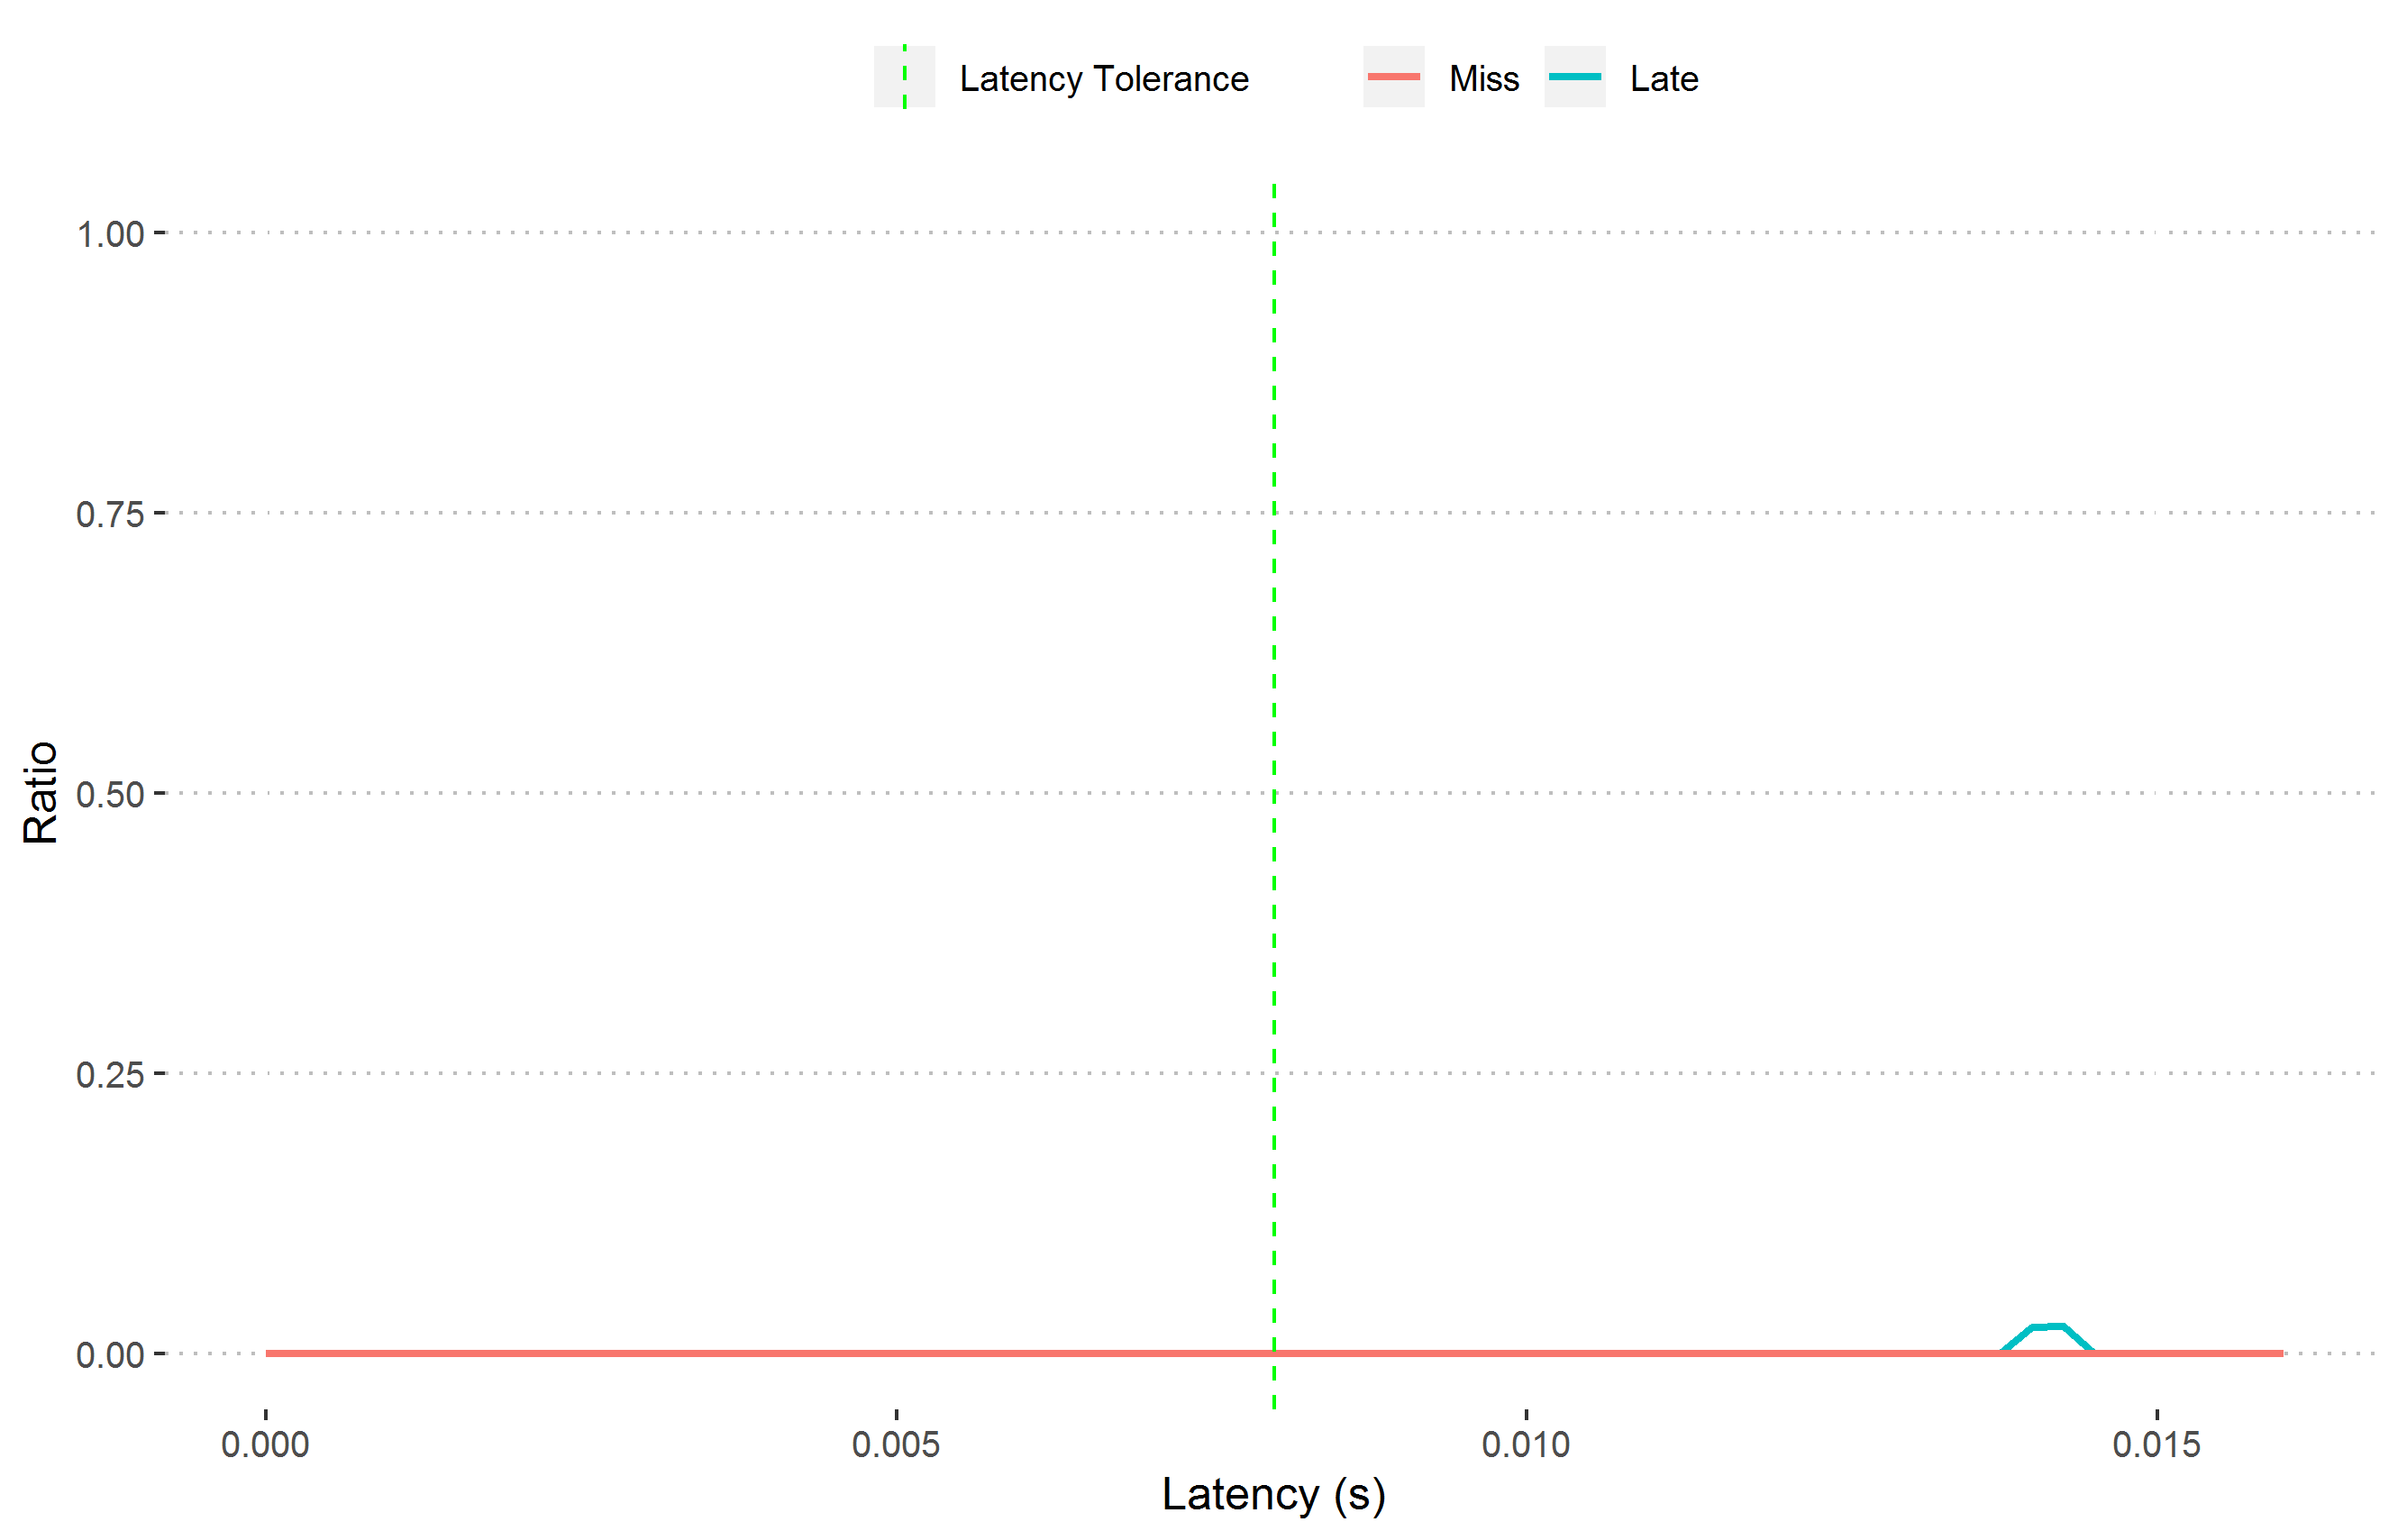
\includegraphics[width=\textwidth]{RatiosVsLatencyMid}
	\caption{Ratio of Late to Correct Collisions and Misses to Total Collision vs. Latency using a latency tolerance of $8ms$. The latency tolerance is marked in a dashed green line.}
	\label{fig_RatioVsLatencyMid}
\end{figure}
\begin{figure}
	\centering
	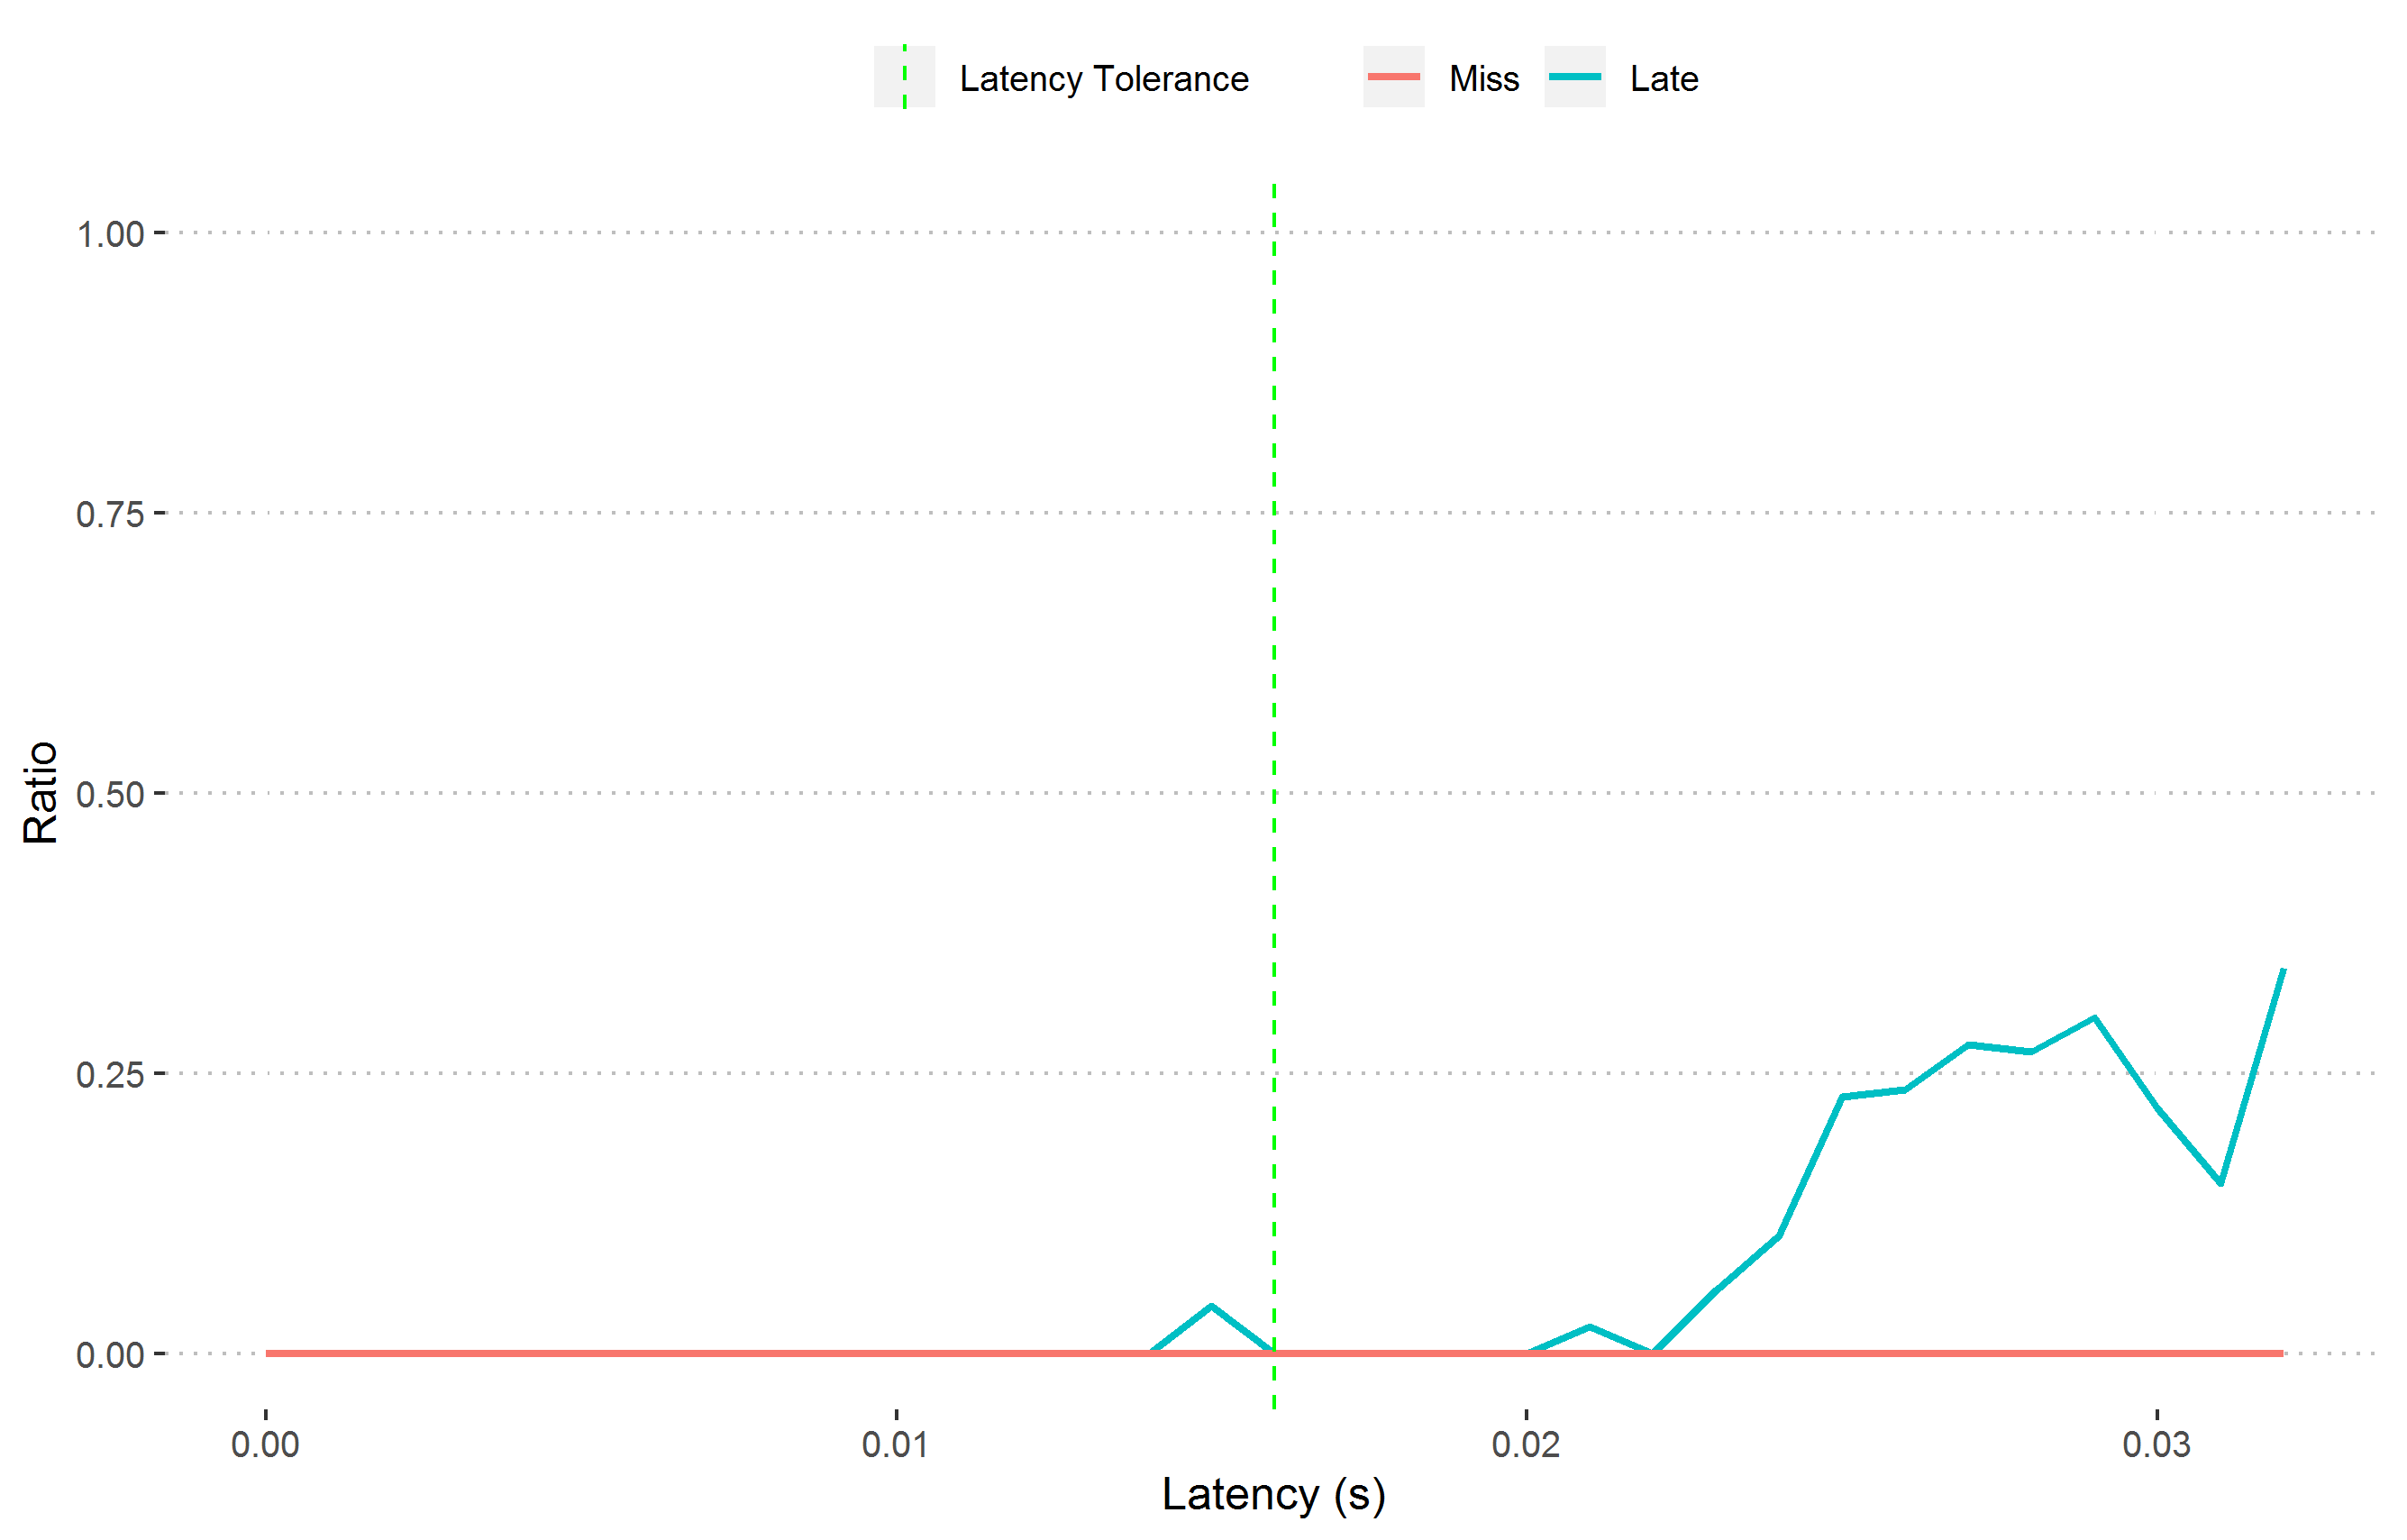
\includegraphics[width=\textwidth]{RatiosVsLatencyHigh}
	\caption{Ratio of Late to Correct Collisions and Misses to Total Collision vs. Latency using a latency tolerance of $16ms$. The latency tolerance is marked in a dashed green line.}
	\label{fig_RatioVsLatencyHigh}
\end{figure}

\begin{figure}
	\centering
	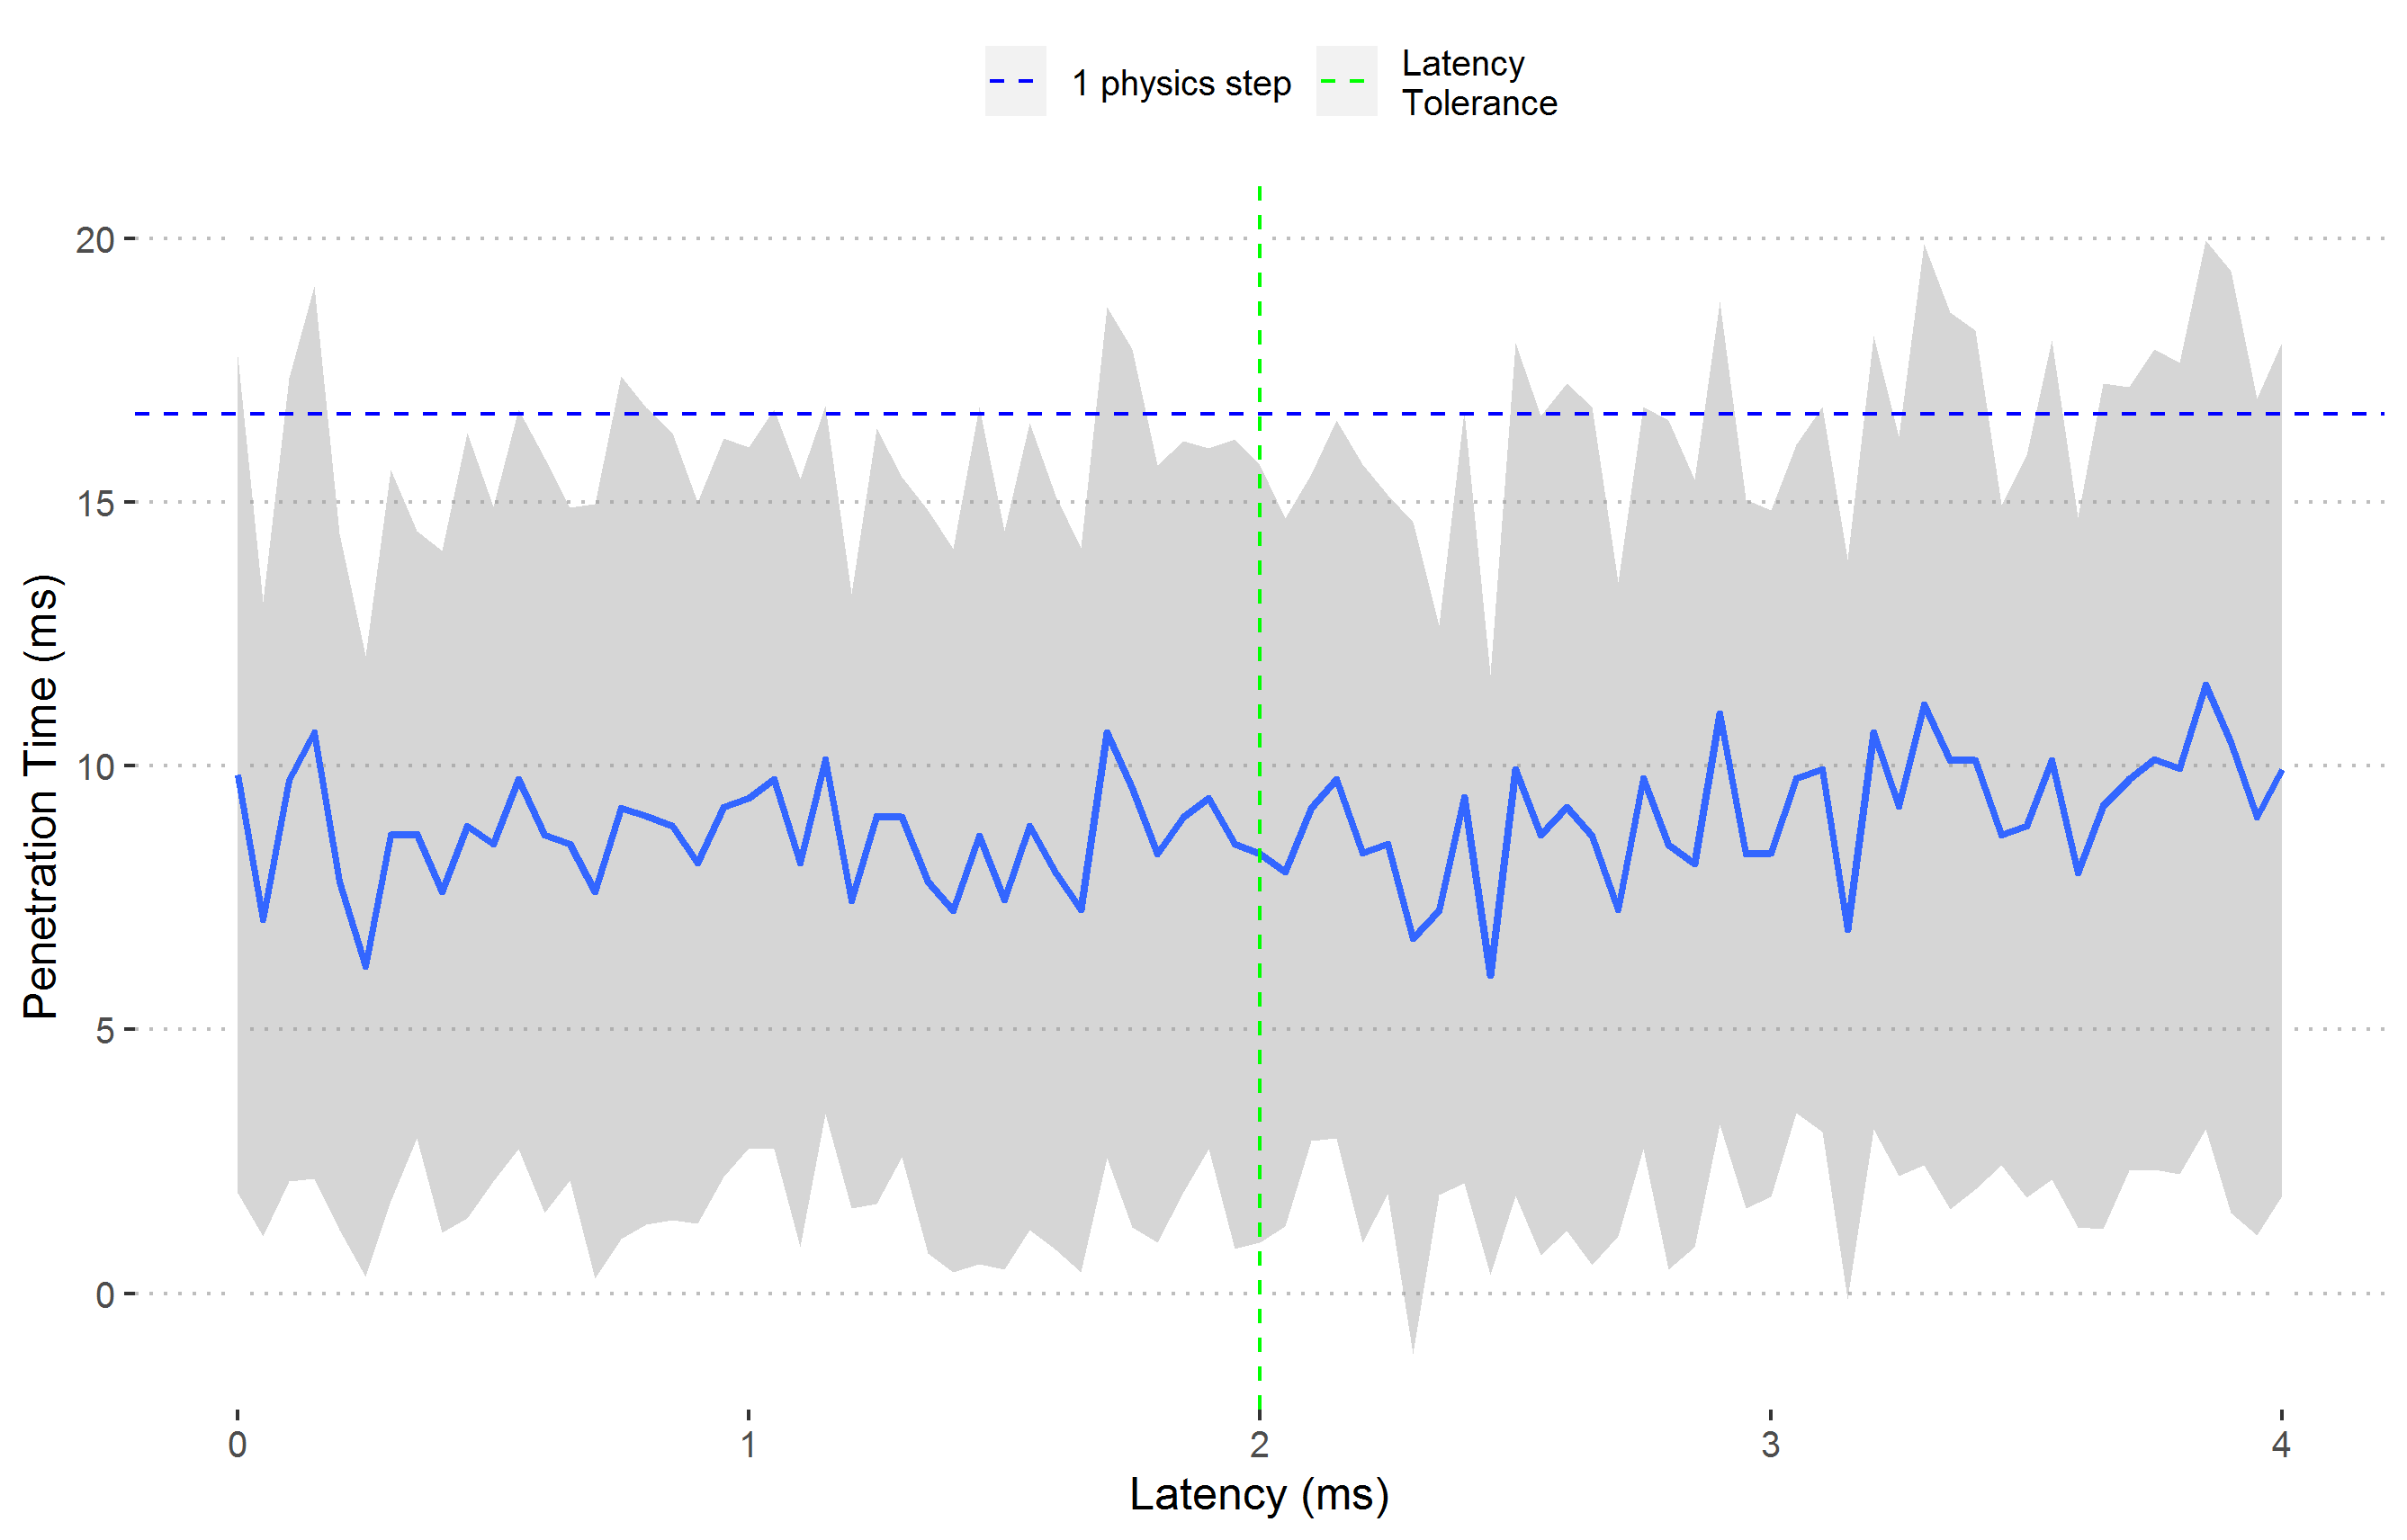
\includegraphics[width=\textwidth]{MeanPenVsLatencyLow}
	\caption{Mean penetration time of objects with $+/-2$ standard deviations with varying latency using a latency tolerance of $2ms$. The maximum expected penetration time of 1 physics step is marked with a dashed blue line. The latency tolerance is marked in a dashed green line.}
	\label{fig_CollisionsPenVsLatencyLow}
\end{figure}
\begin{figure}
	\centering
	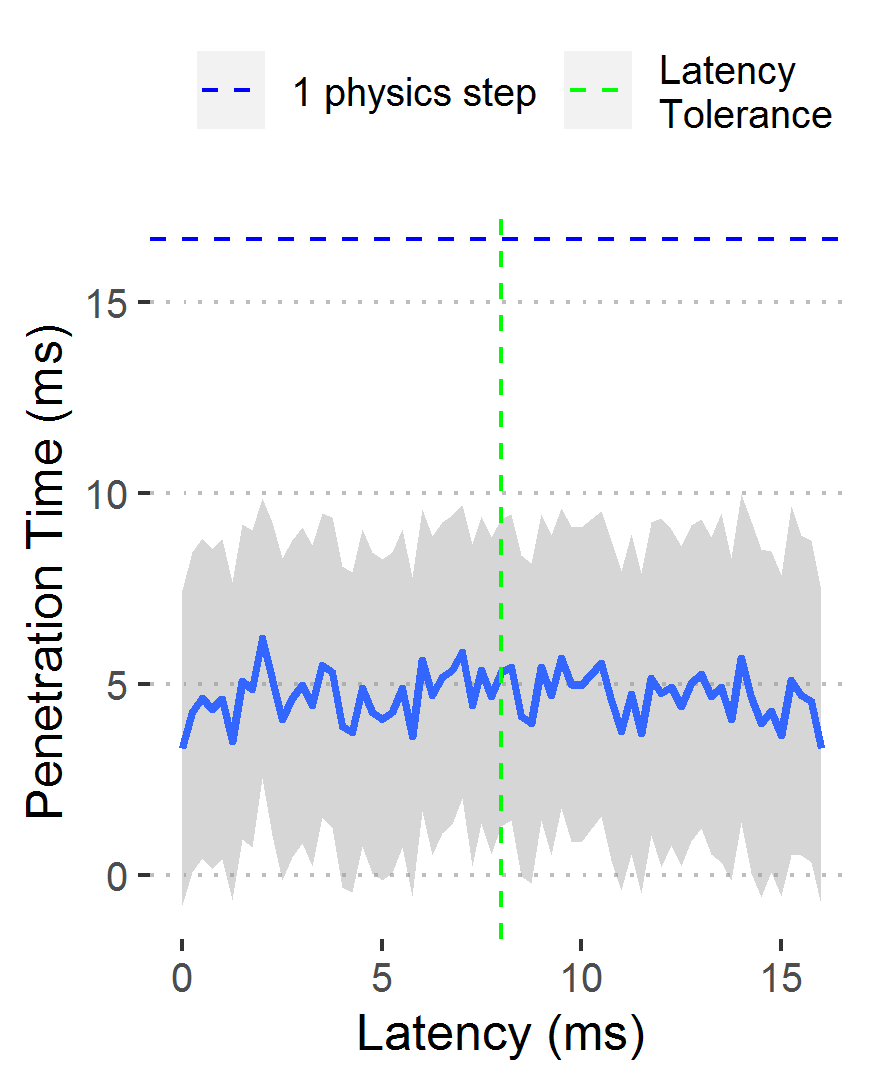
\includegraphics[width=\textwidth]{MeanPenVsLatencyMid}
	\caption{Mean penetration time of objects with $+/-2$ standard deviations with varying latency using a latency tolerance of $8ms$. The maximum expected penetration time of 1 physics step is marked with a dashed blue line. The latency tolerance is marked in a dashed green line.}
	\label{fig_CollisionsPenVsLatencyMid}
\end{figure}
\begin{figure}
	\centering
	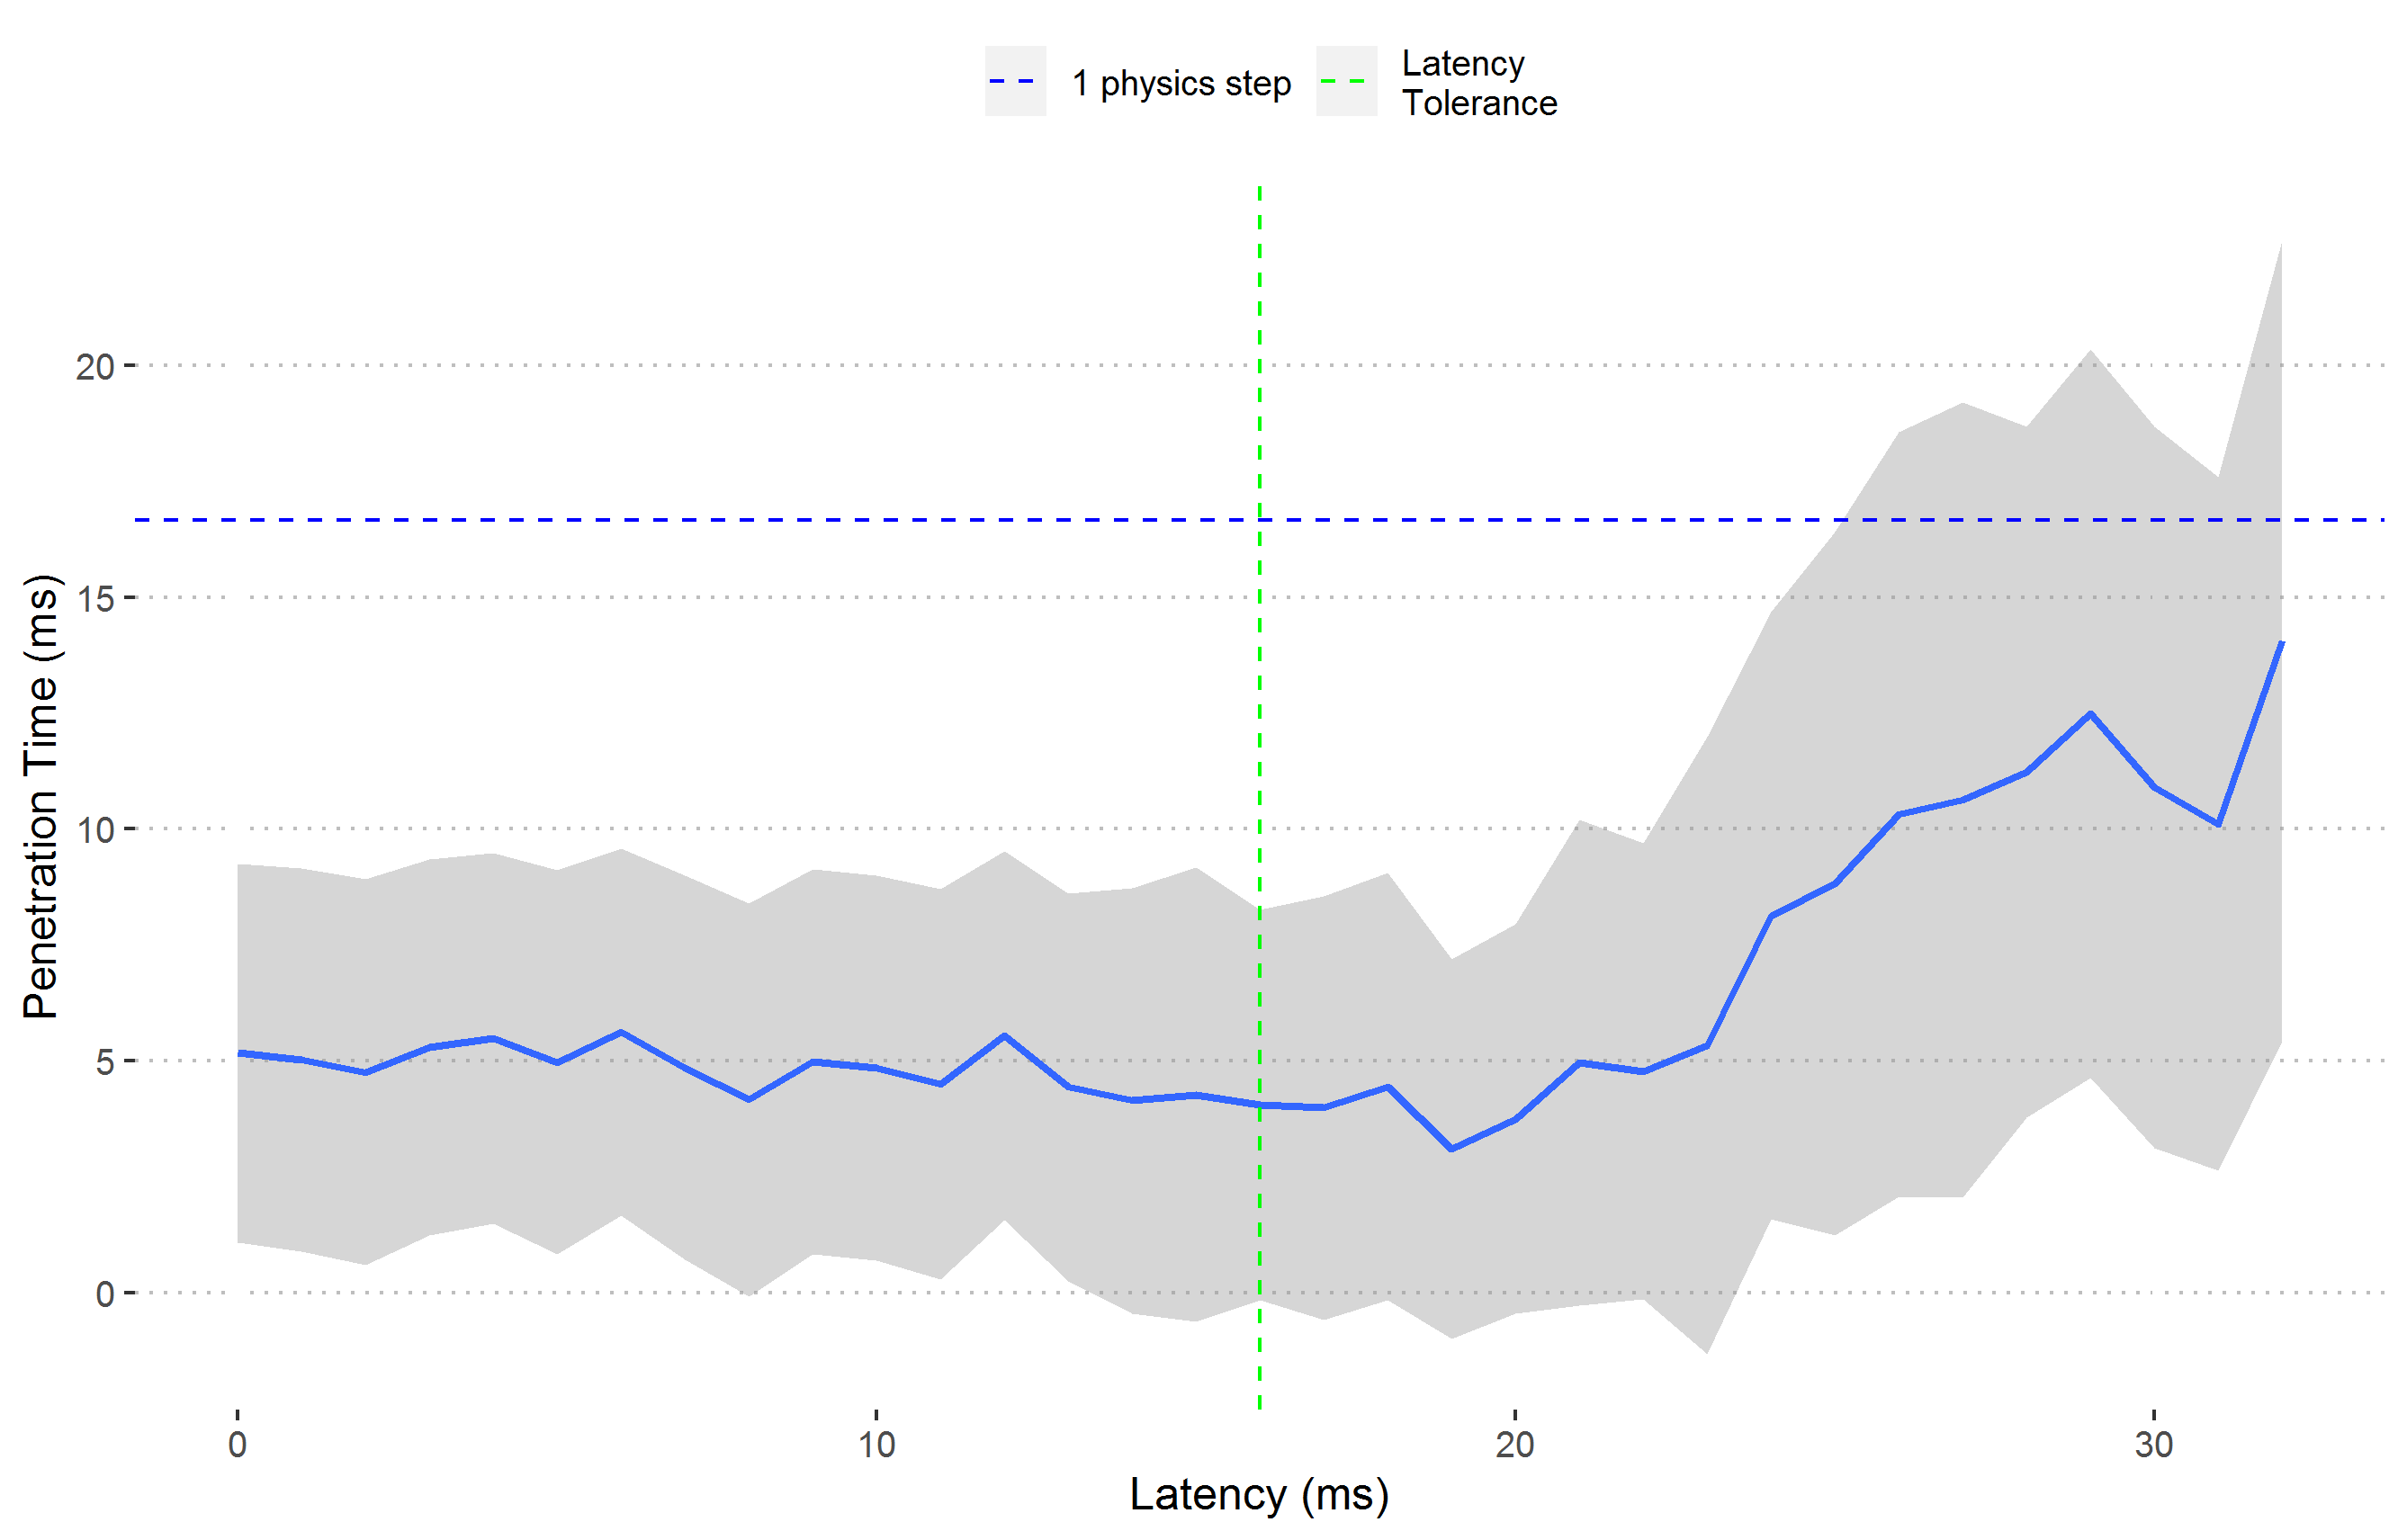
\includegraphics[width=\textwidth]{MeanPenVsLatencyHigh}
	\caption{Mean penetration time of objects with $+/-2$ standard deviations with varying latency using a latency tolerance of $16ms$. The maximum expected penetration time of 1 physics step is marked with a dashed blue line. The latency tolerance is marked in a dashed green line.}
	\label{fig_CollisionsPenVsLatencyHigh}
\end{figure}

%\begin{figure}
%\centering
%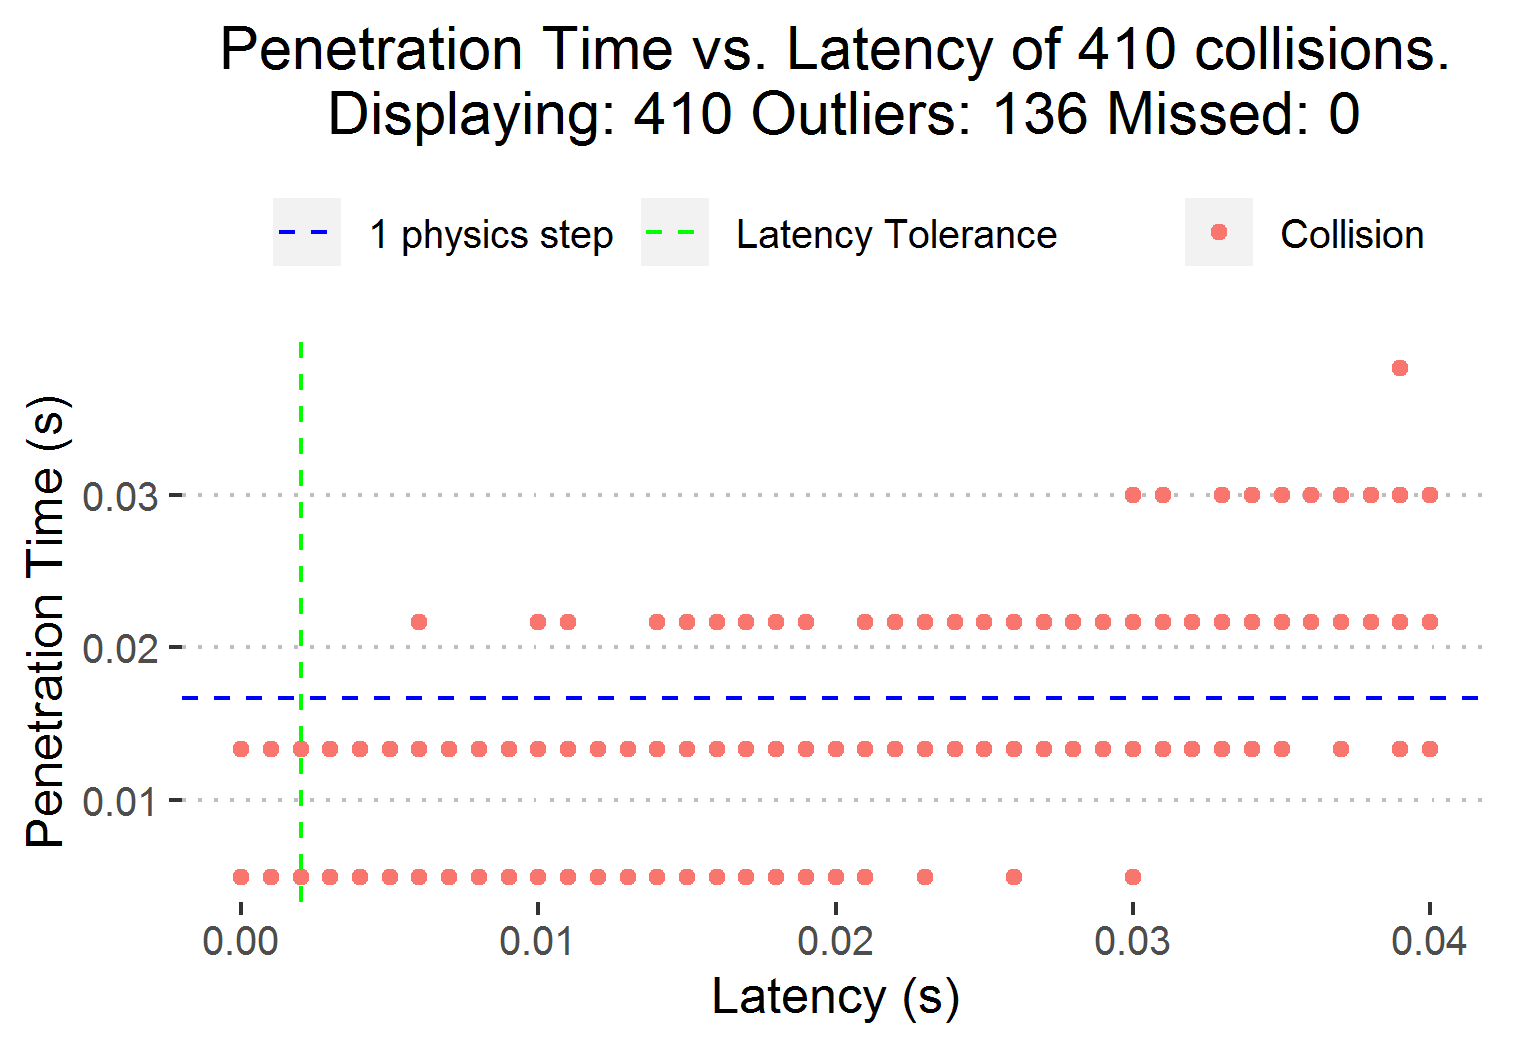
\includegraphics[width=\textwidth]{CollisionsPenVsLatency}
%\caption{Penetration time of objects with varying latency. Each red point represents one or more collisions. The maximum expected penetration time of 1 physics steps is marked with a dashed blue line. The latency tolerance is marked in a dashed green line. The number and magnitude of errors increases as latency increases beyond the tolerance.}
%\label{fig_CollisionsPenVsLatency}
%\end{figure}
%
%\begin{figure}
%\centering
%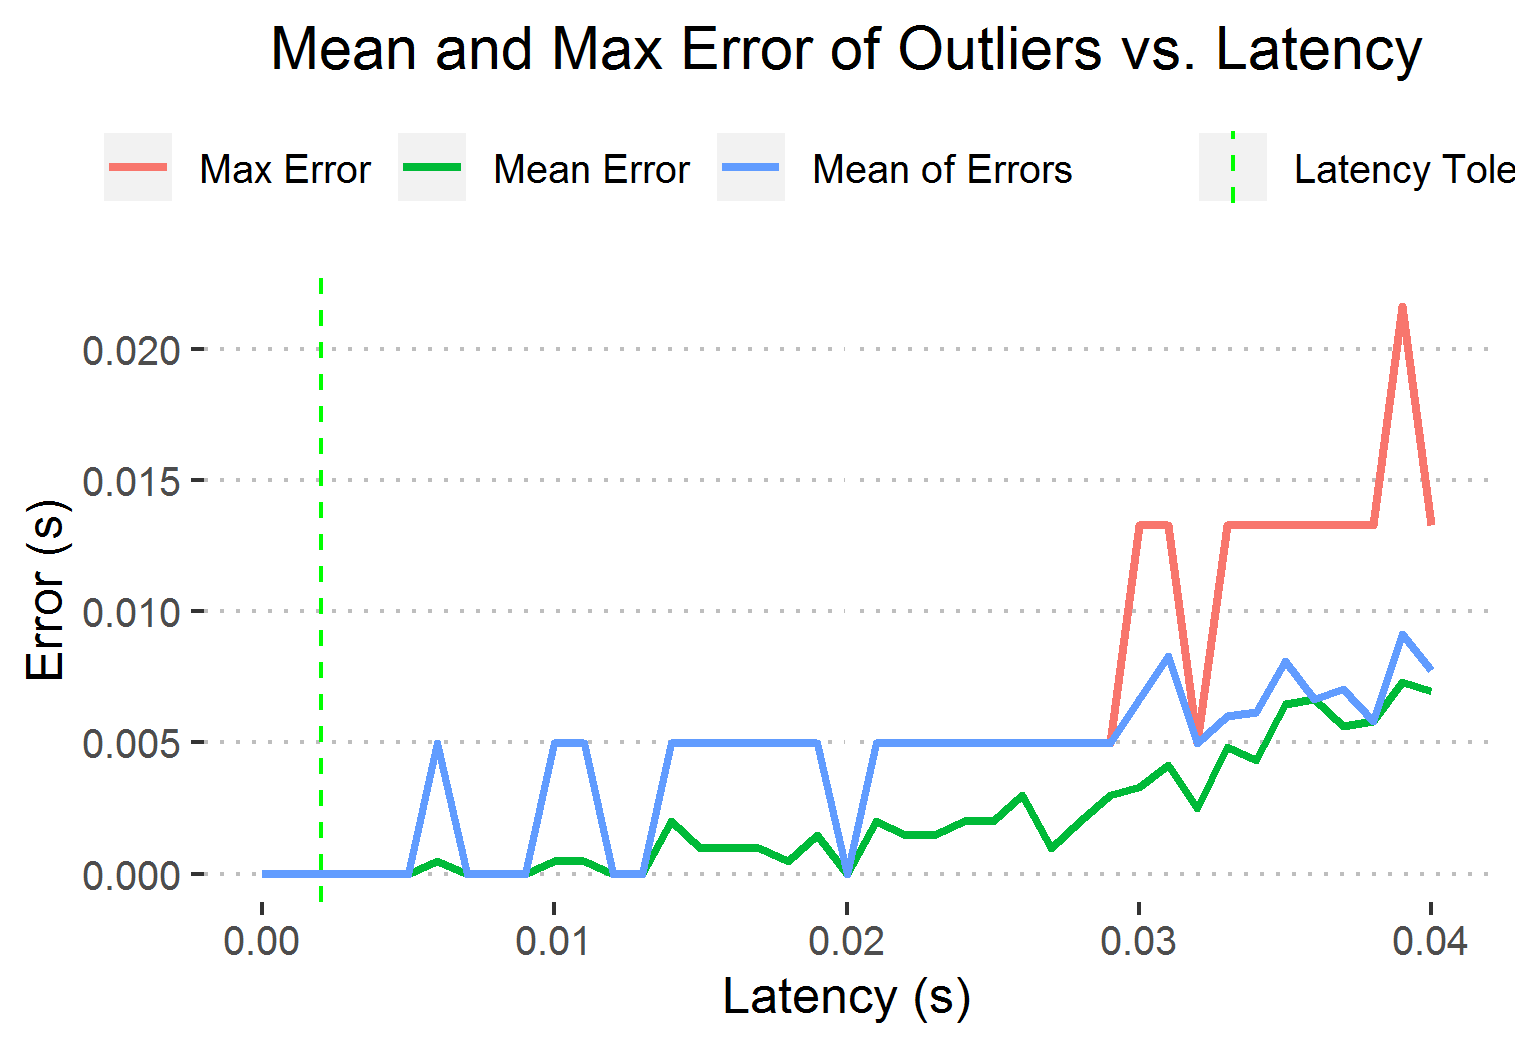
\includegraphics[width=\textwidth]{MeanMaxErrorVsLatency}
%\caption{The mean and max of collision errors with varying latency}
%\label{fig_MeanMaxErrorVsLatency}
%\end{figure}
%
%\begin{figure}
%\centering
%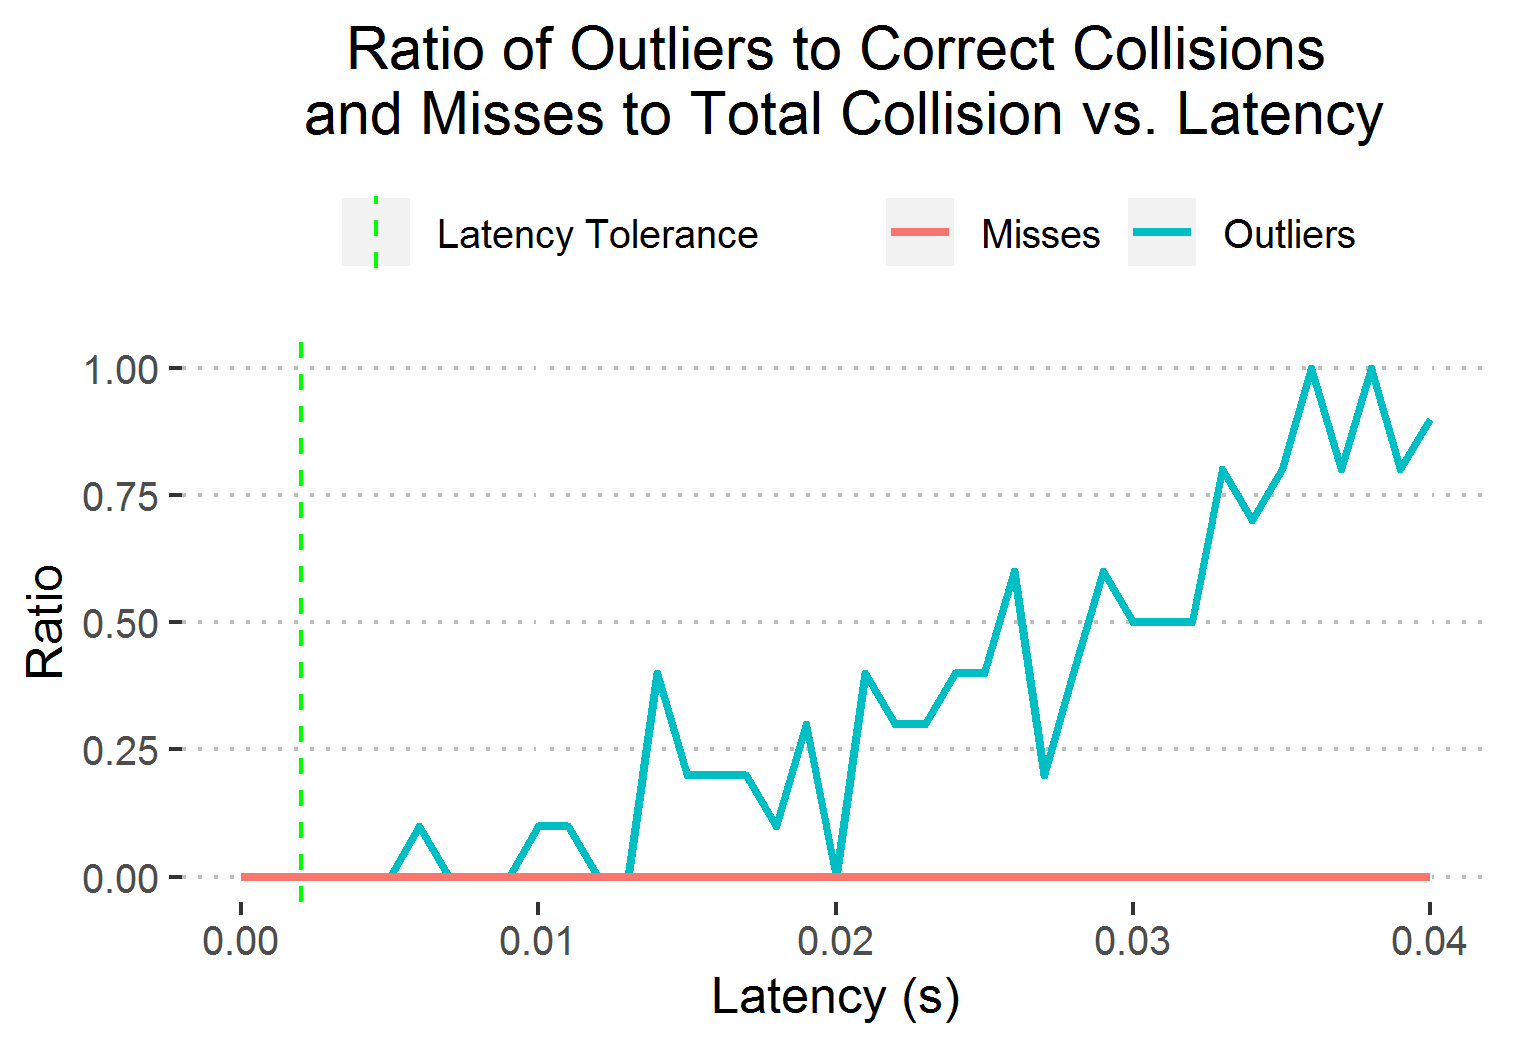
\includegraphics[width=\textwidth]{RatiosVsLatency}
%\caption{The ratios of erroneous collisions to correct collisions and missed collisions to total collisions with varying latency}
%\label{fig_RatiosVsLatency}
%\end{figure}

\subsubsection{Varying Frame-Time}

In this experiment the frame-time was varied from $0ms$ to double the frame-time tolerance for the following frame-times: $8.33ms$ $(120Hz)$; $15ms$ $(66.67Hz)$ and $33.33ms$ $(30Hz)$. Increments of $1ms$, $1ms$ and $2ms$ were used respectively. The frame-time used is target frame time, in reality frame-time cannot be equal to exactly $0ms$.

\begin{figure}
	\centering
	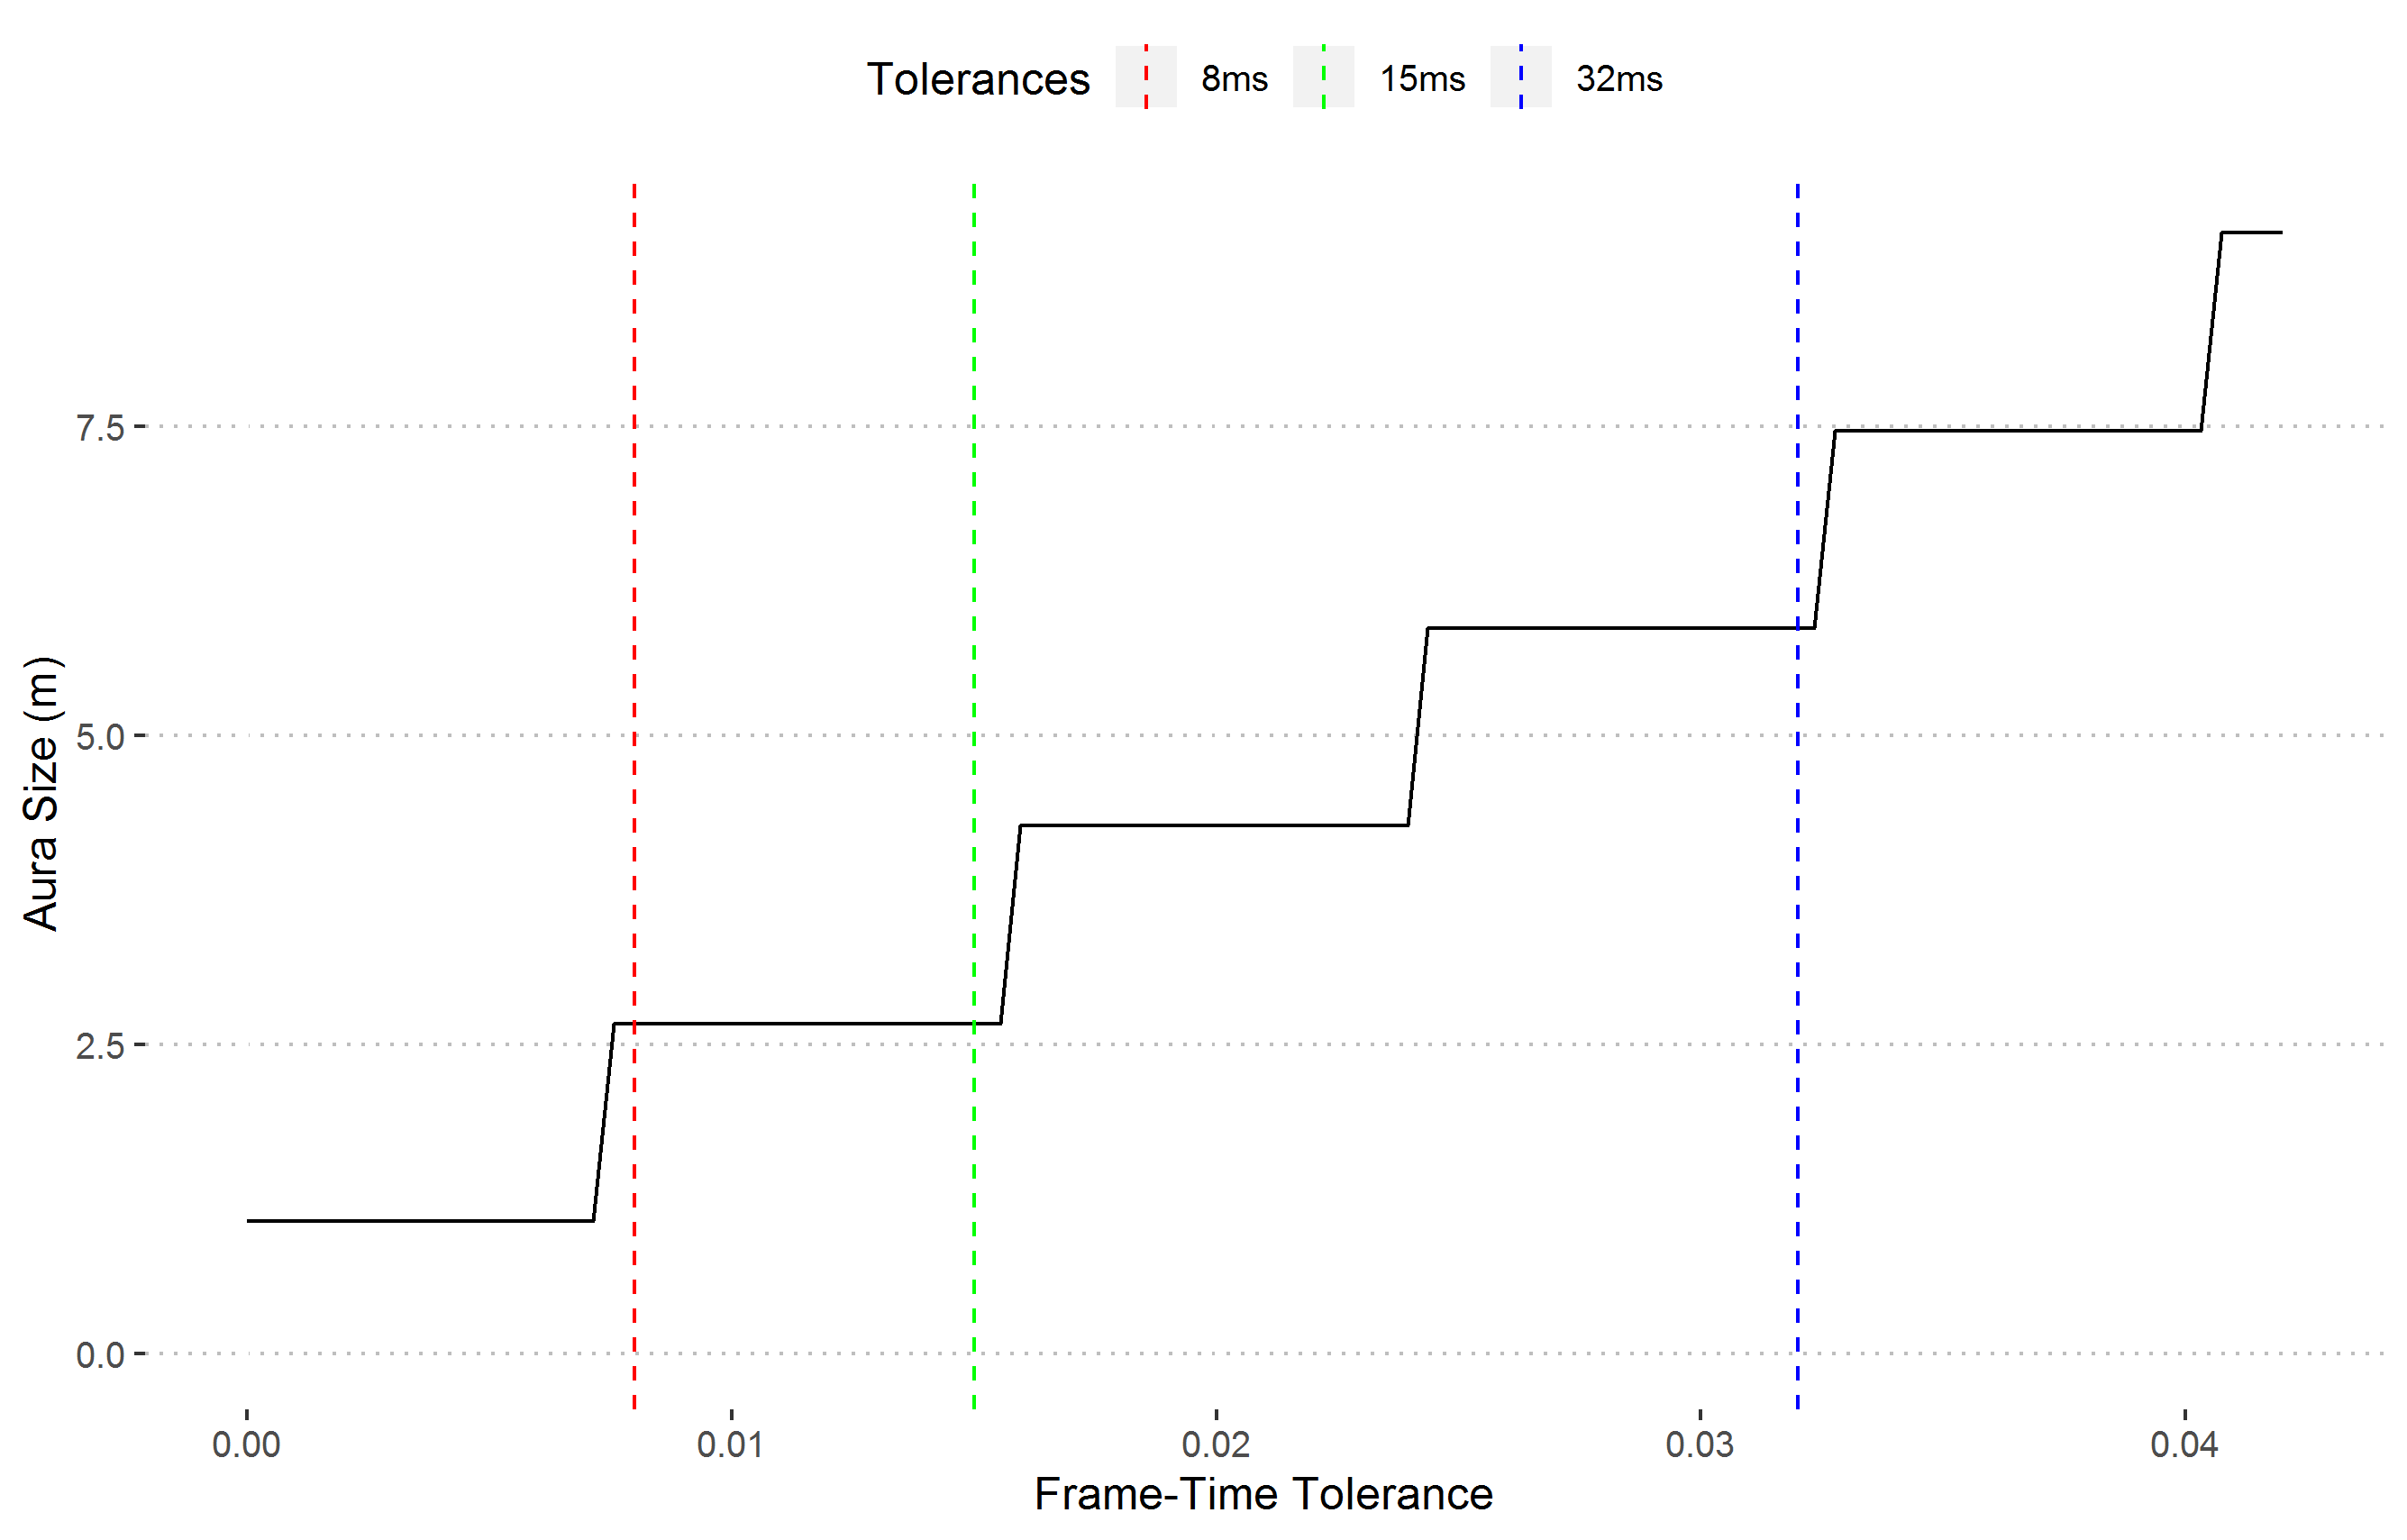
\includegraphics[width=\textwidth]{FrameAuraSizes}
	\caption{Size of aura vs. frame-time tolerance. The frame-time tolerances used are marked in dashed lines}
	\label{fig_FrameTimeAuraSize}
\end{figure}

Fig. \ref{fig_FrameTimeAuraSize} shows the size of the aura (not including the bounding sphere of the object) vs increasing frame-time tolerance, calculated using equation \ref{auraEquation}. The aura size increases discretely with frame-time tolerance, therefore we expect late collisions to begin only once the the actual frame-time is higher than the maximum frame-time the current aura size tolerates. In the varying frame-time experiments, this will be when frame-time reaches $16ms$ for the $8ms$ and $15ms$ tolerance experiments and $32ms$ for the $32ms$ tolerance experiment. Note that late collisions are not expected for the $8ms$ experiment, as $16ms$ frame-time is not exceeded. False-positives are expected due to the frame-time delay method and should increase as frame-time increases.

\begin{figure}
	\centering
	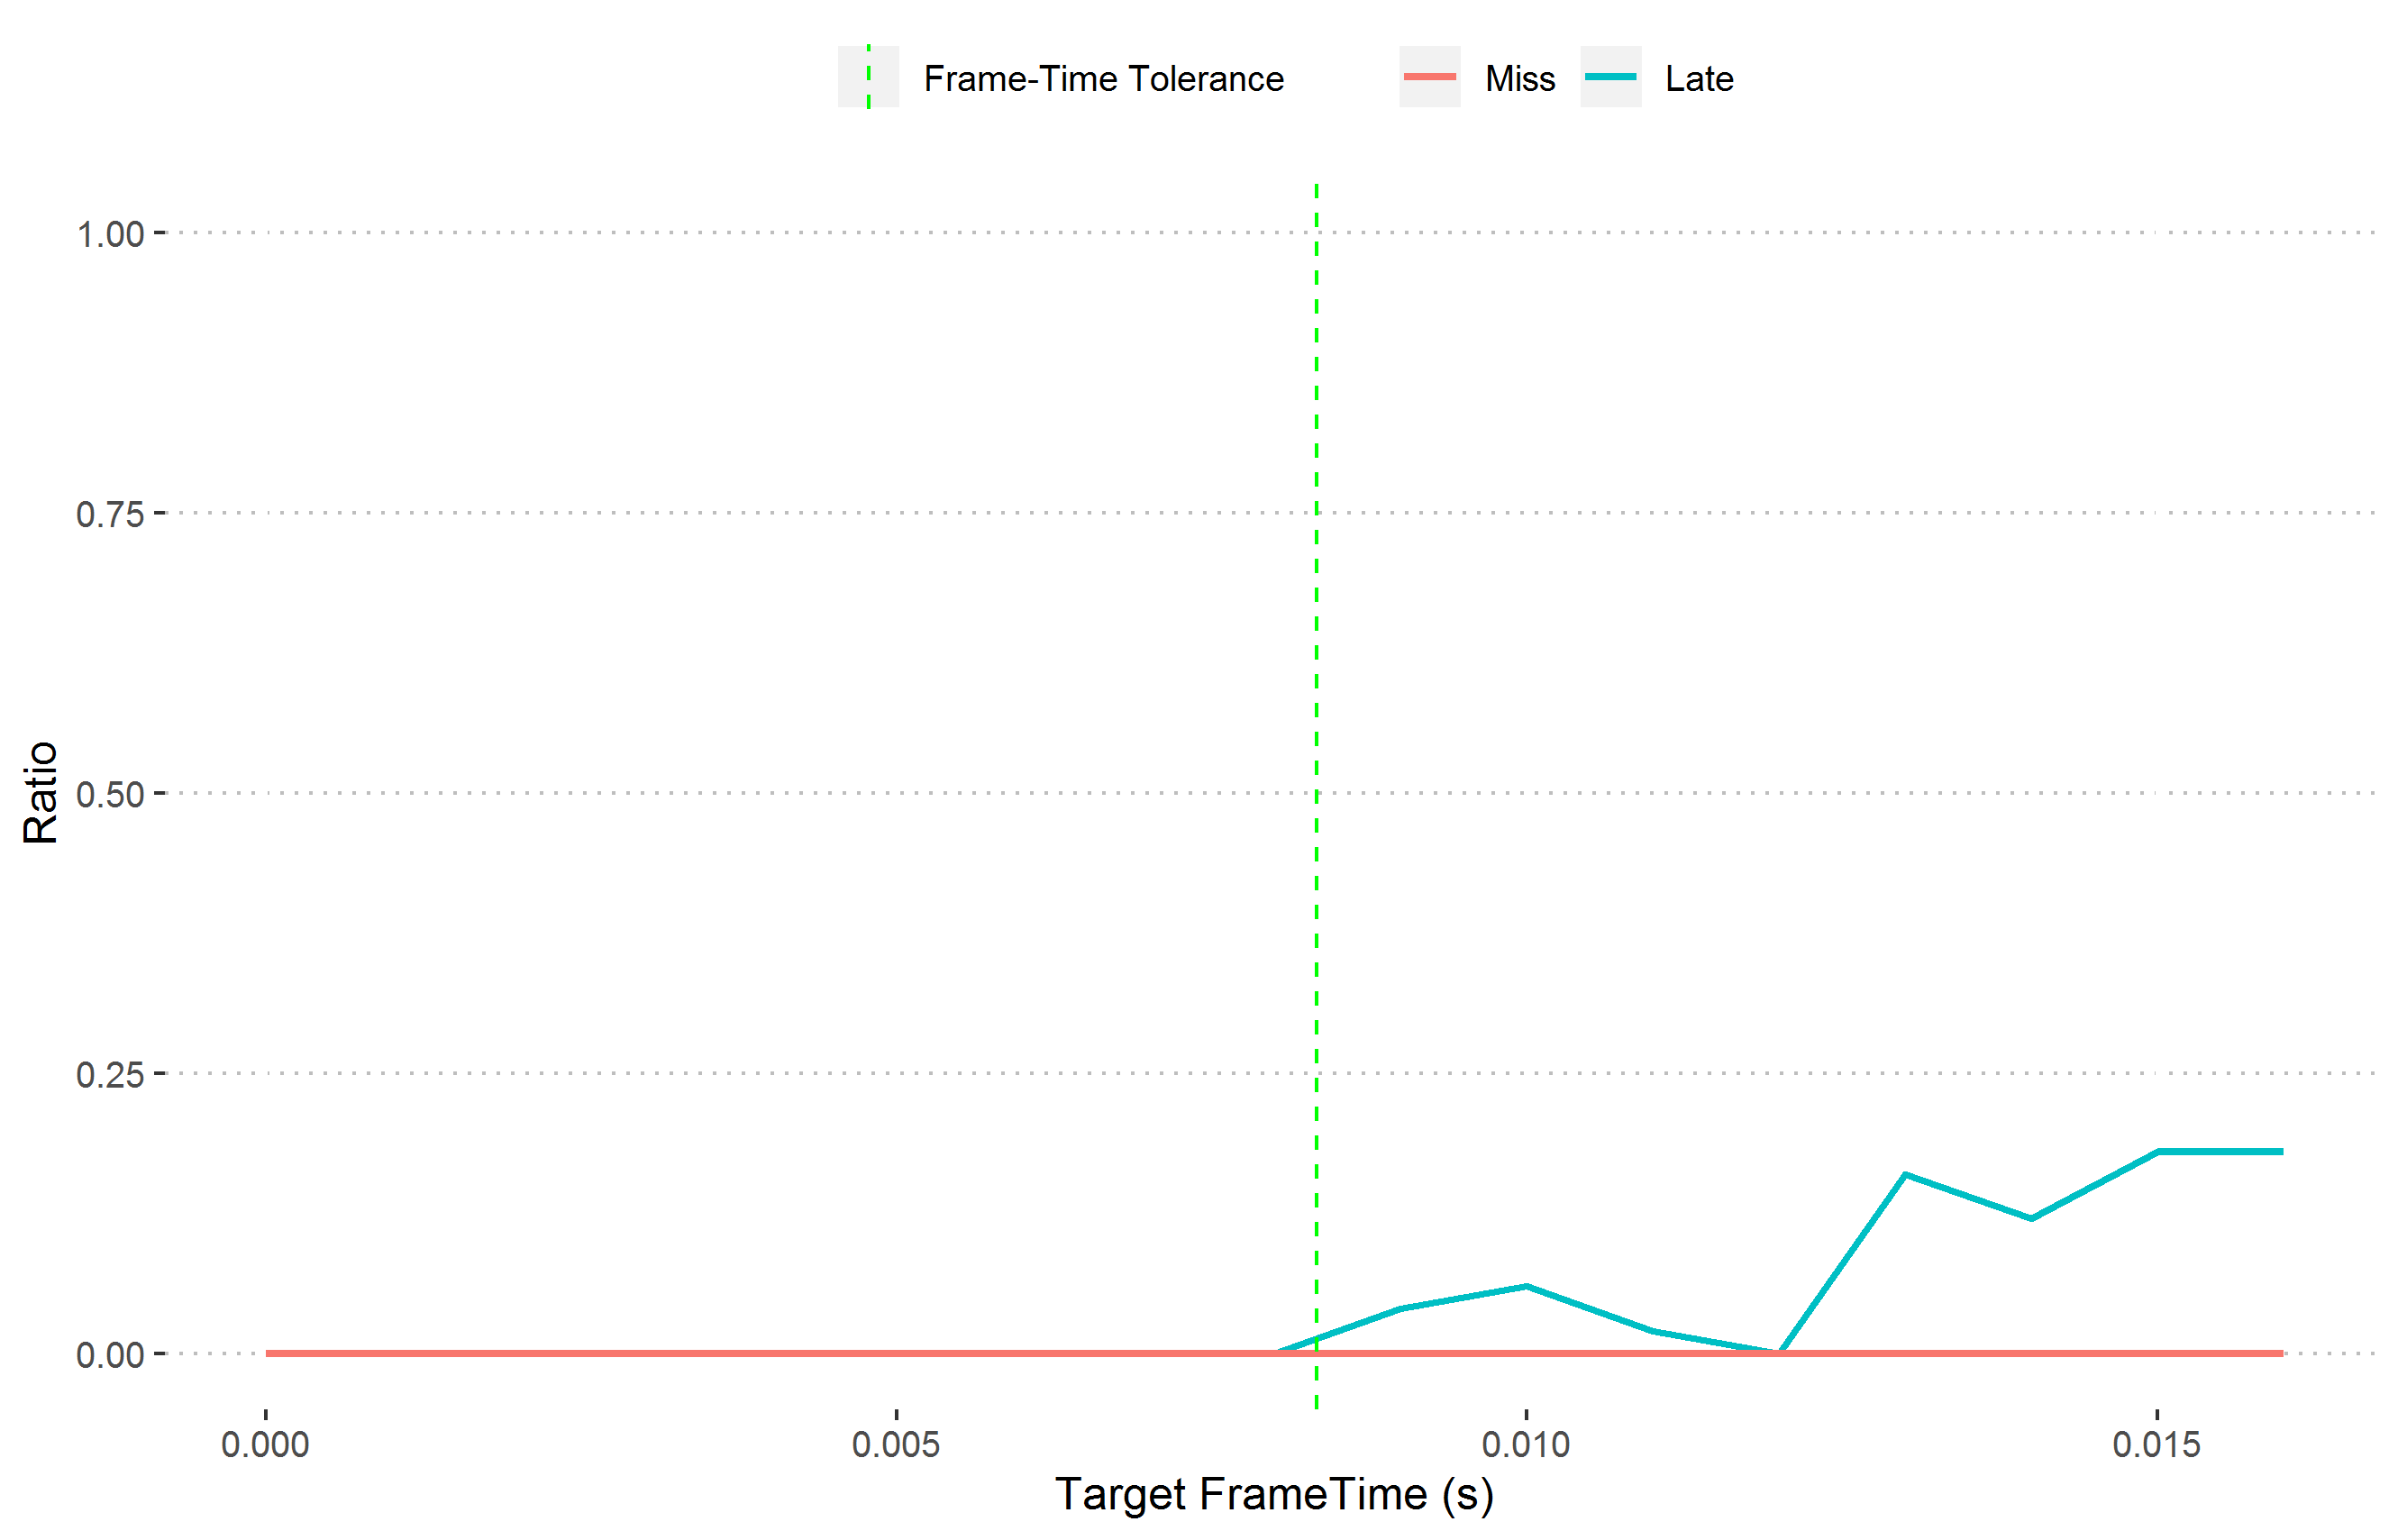
\includegraphics[width=\textwidth]{RatiosVsFrameTimeLow}
	\caption{Ratio of Late to Correct Collisions and Misses to Total Collision vs. frame-time using a frame-time tolerance of $8ms$. The frame-time tolerance is marked in a dashed green line.}
	\label{fig_RatioVsFrameTimeLow}
\end{figure}
\begin{figure}
	\centering
	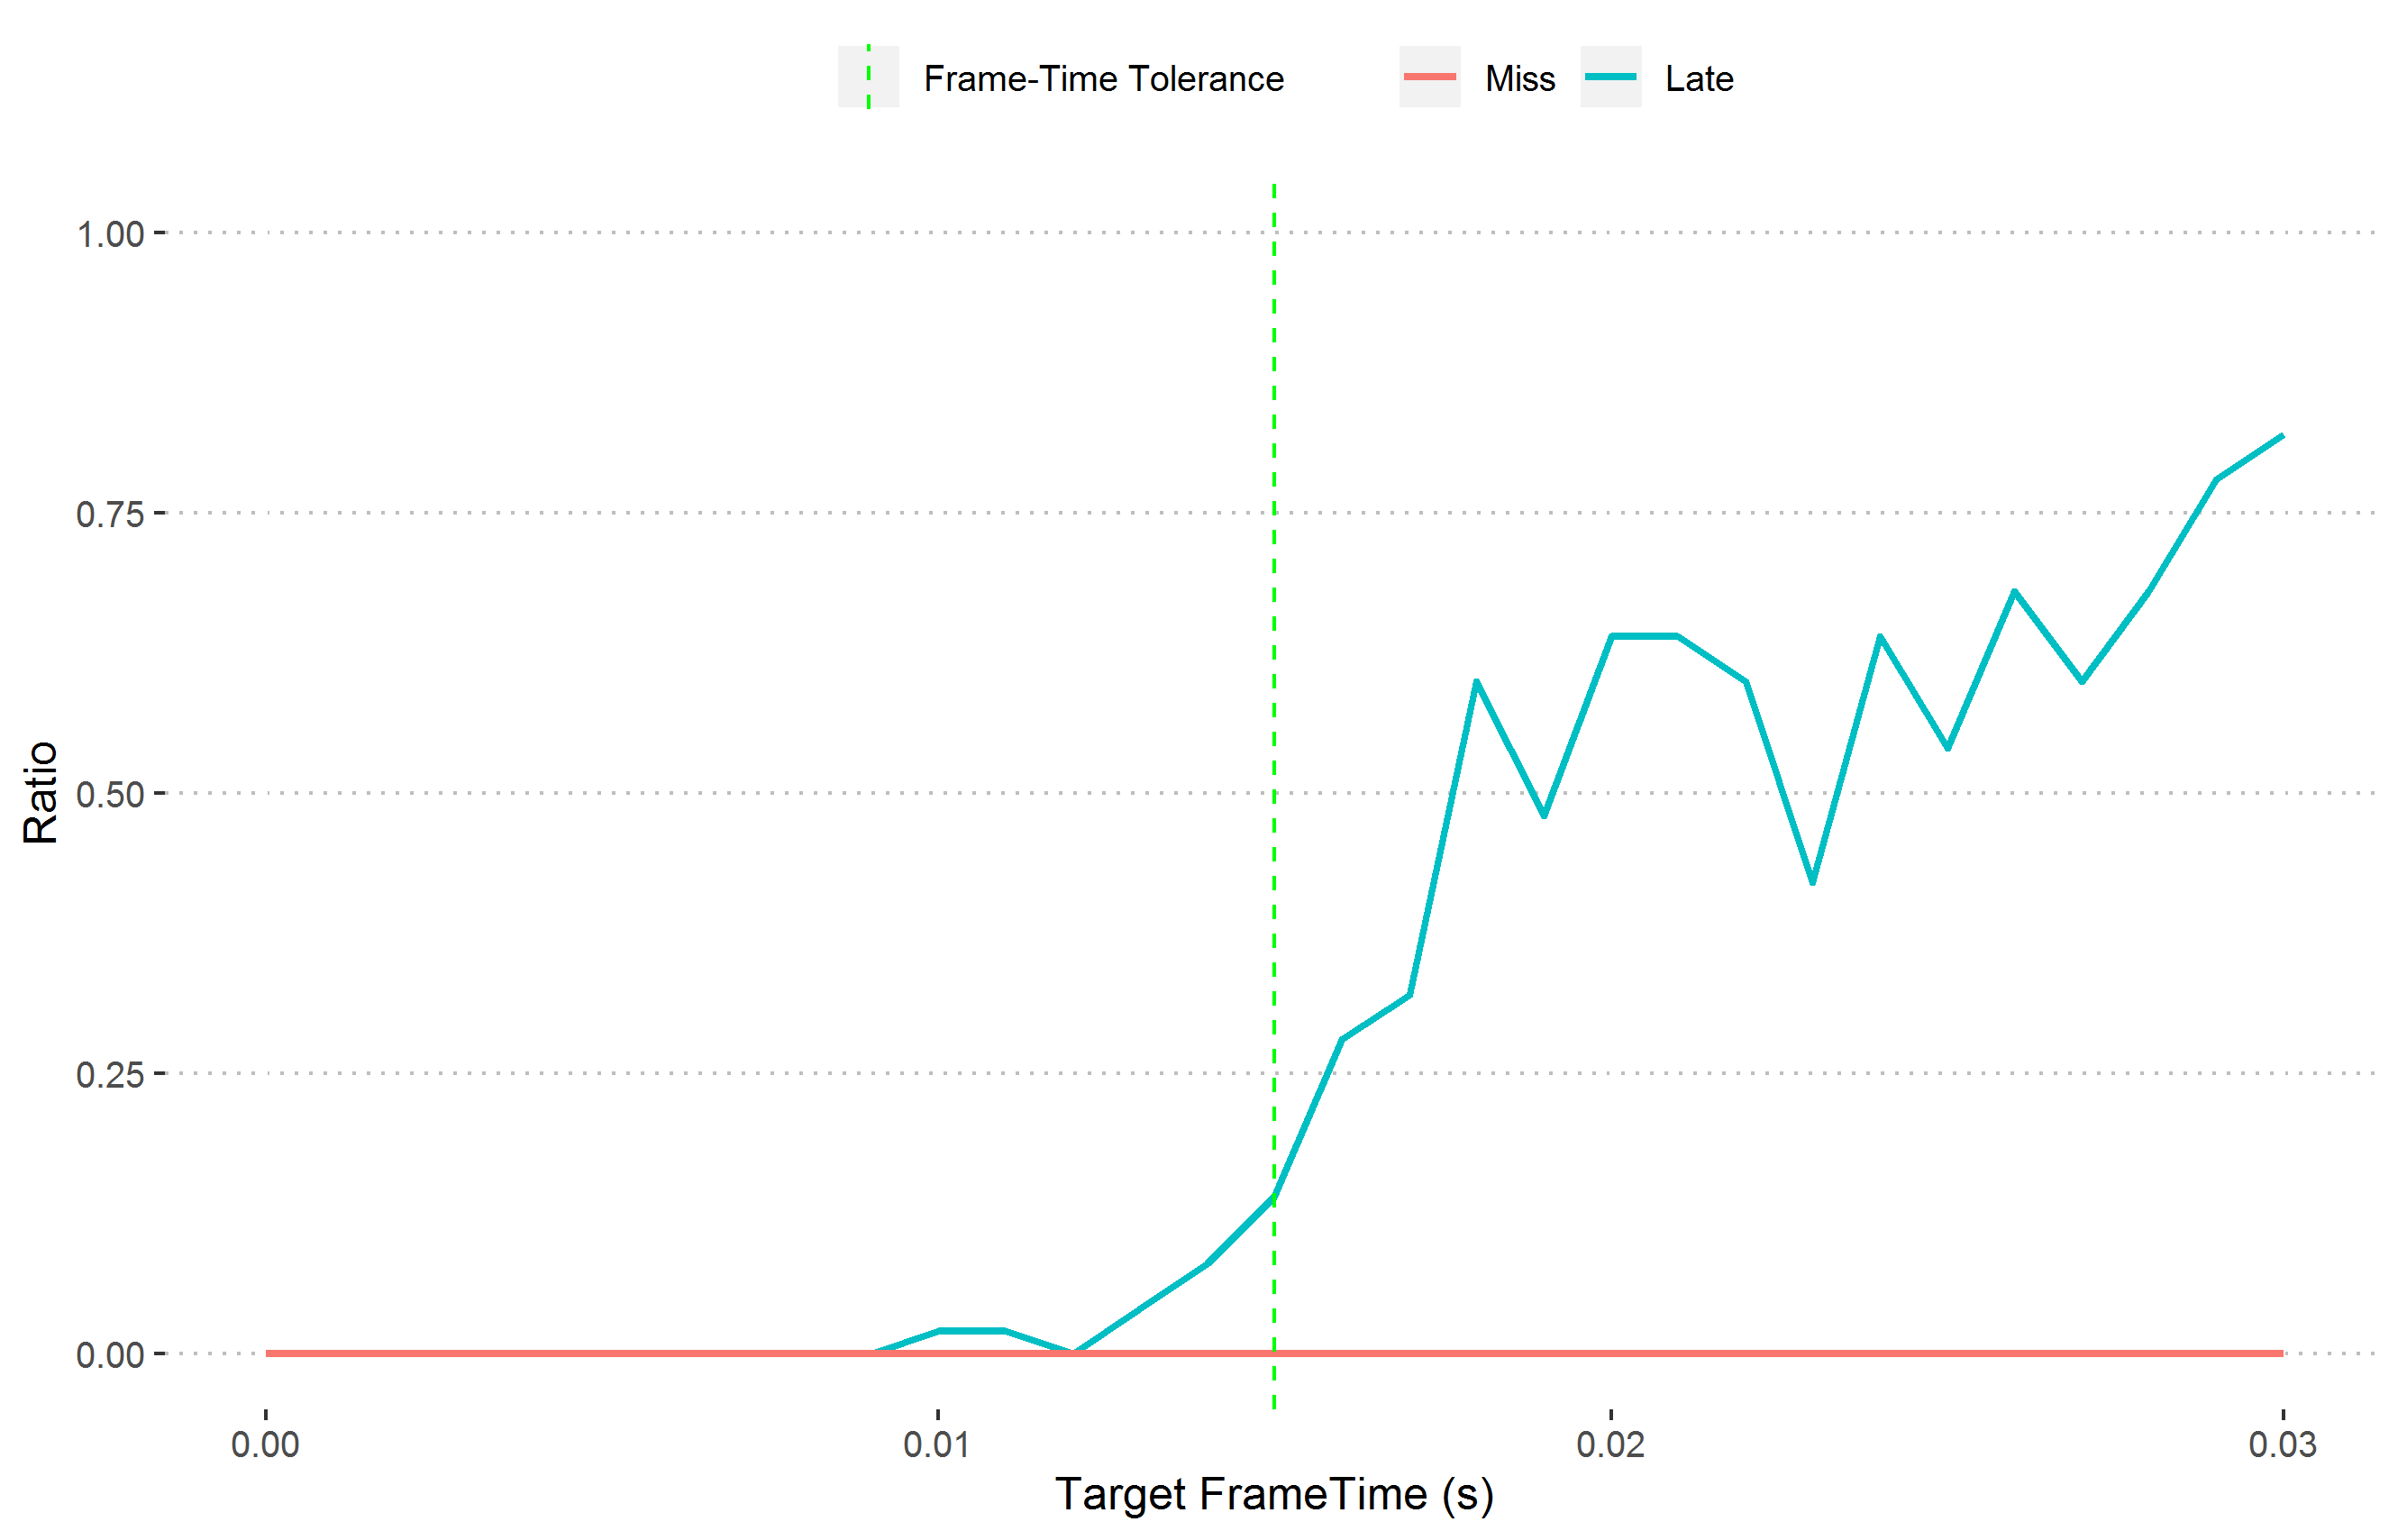
\includegraphics[width=\textwidth]{RatiosVsFrameTimeMid}
	\caption{Ratio of Late to Correct Collisions and Misses to Total Collision vs. frame-time using a frame-time tolerance of $15ms$. The frame-time tolerance is marked in a dashed green line.}
	\label{fig_RatioVsFrameTimeMid}
\end{figure}
\begin{figure}
	\centering
	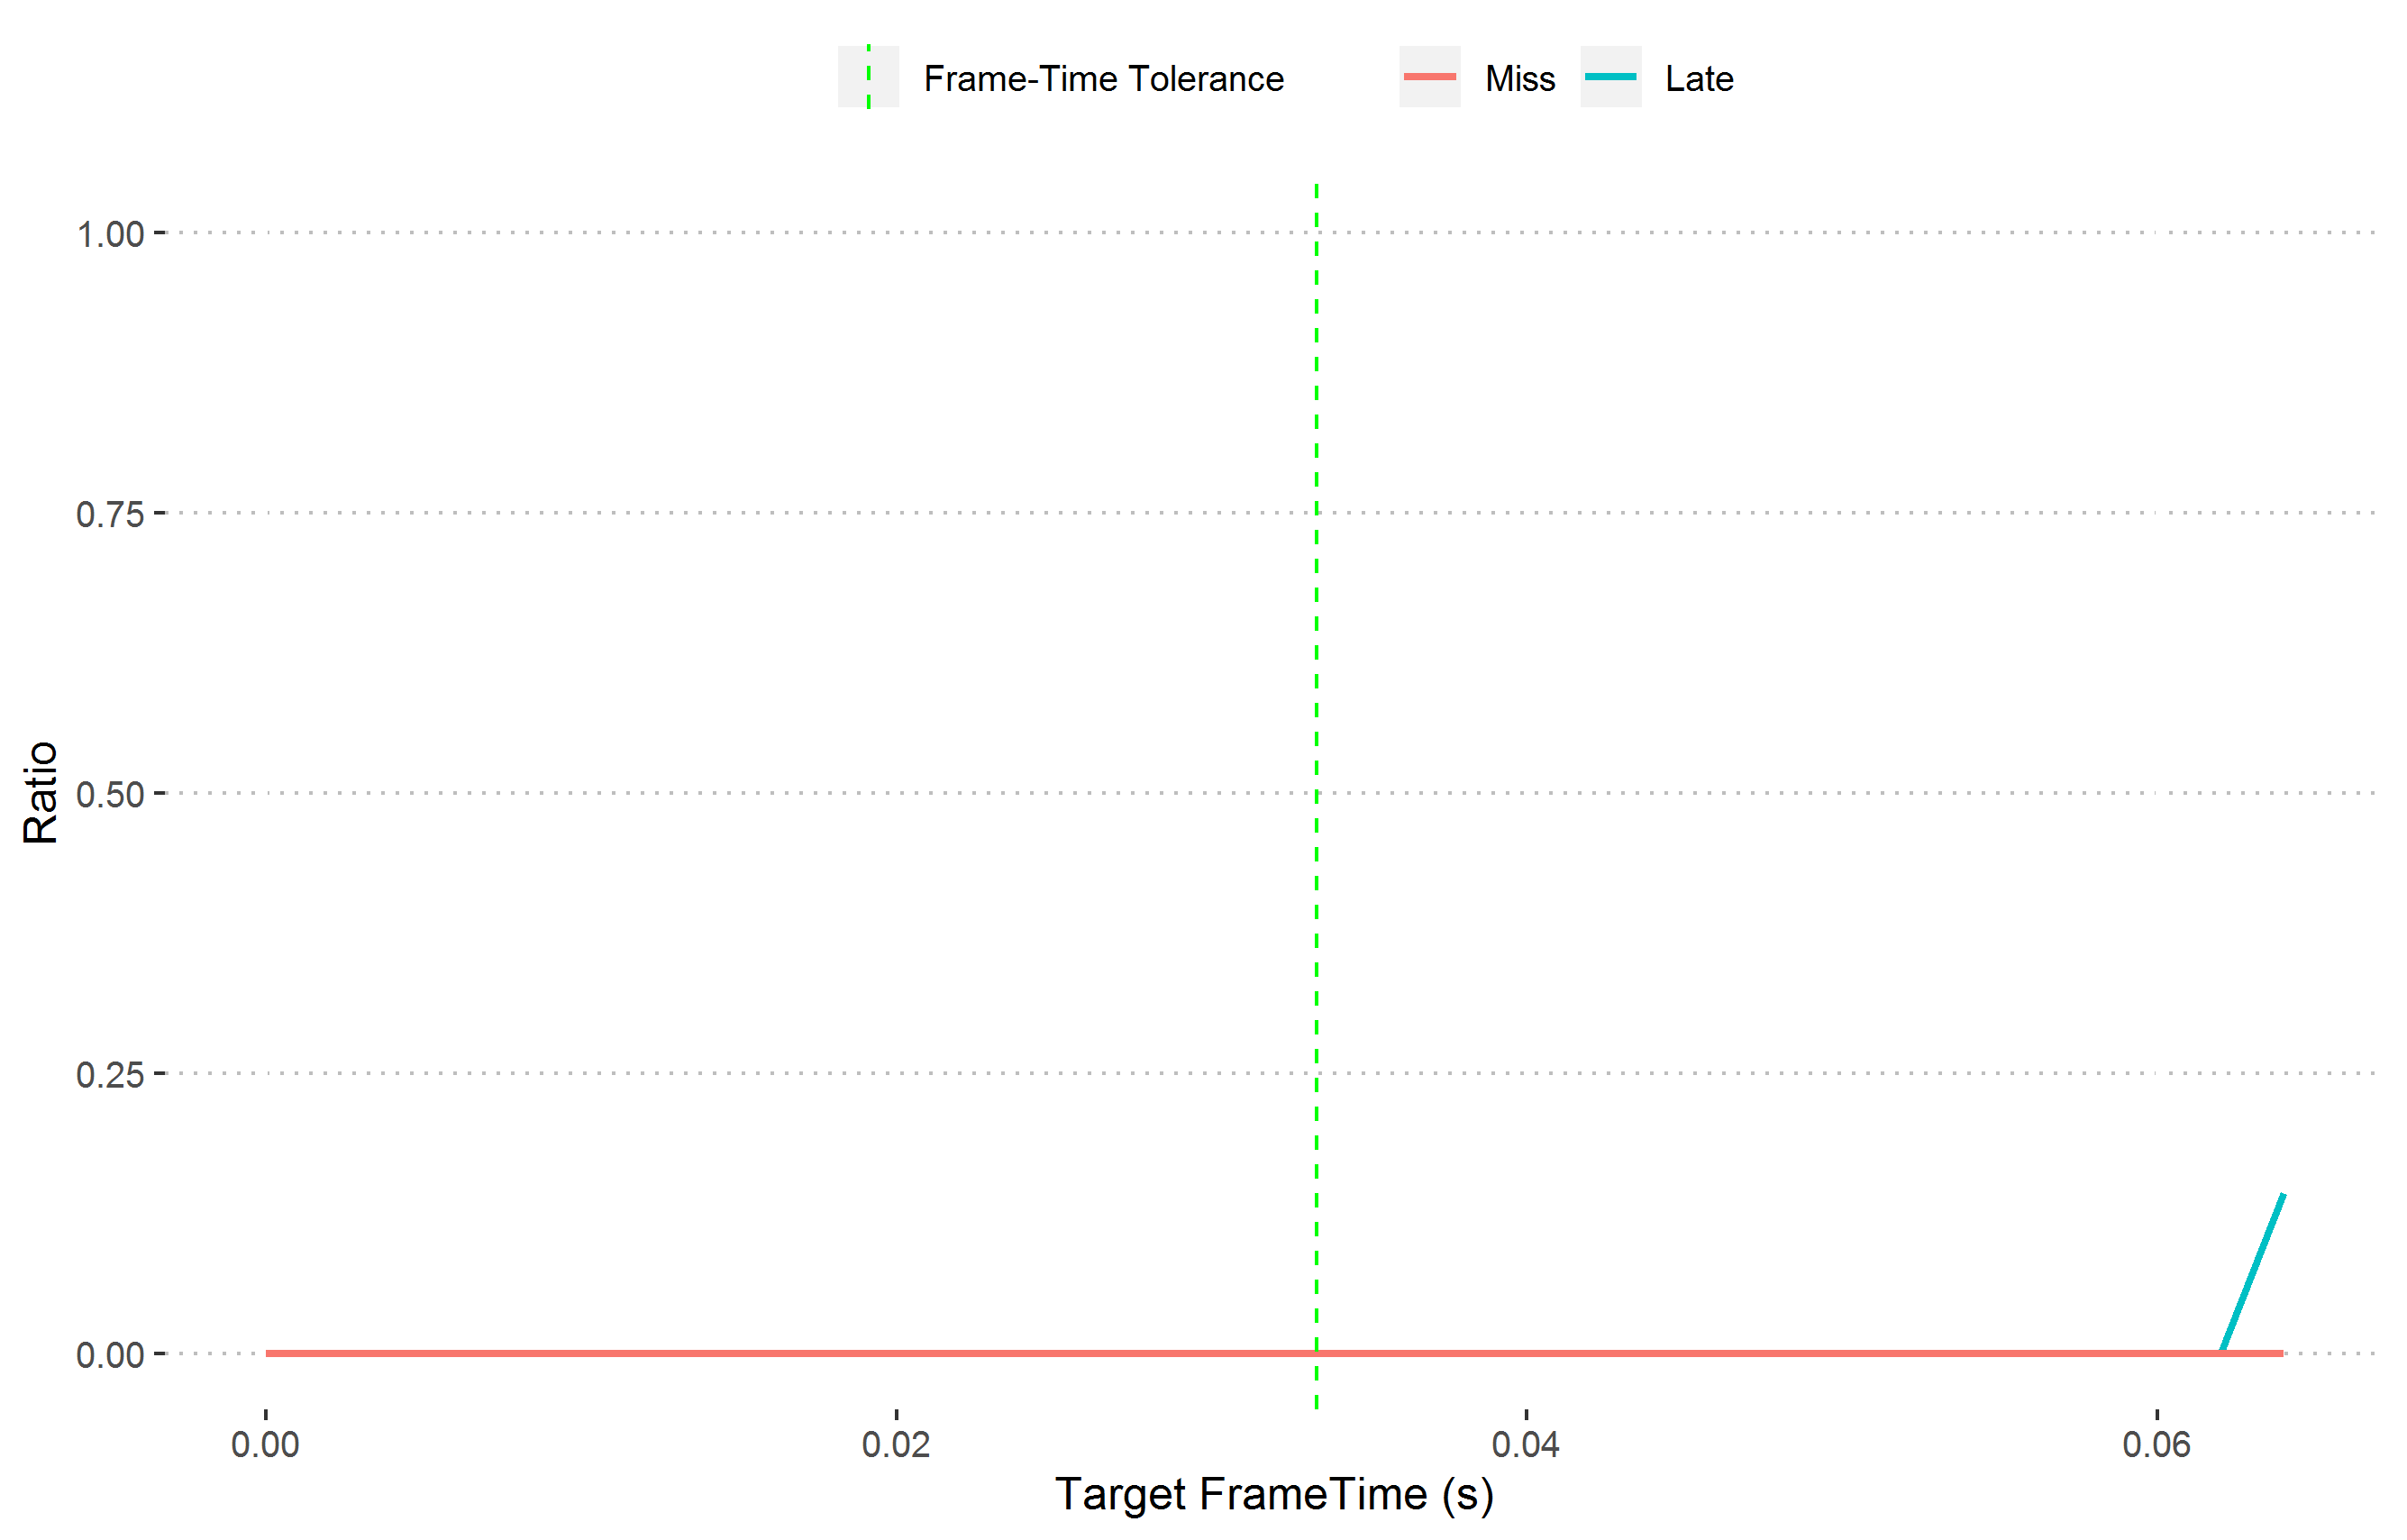
\includegraphics[width=\textwidth]{RatiosVsFrameTimeHigh}
	\caption{Ratio of Late to Correct Collisions and Misses to Total Collision vs. frame-time using a frame-time tolerance of $32ms$. The frame-time tolerance is marked in a dashed green line.}
	\label{fig_RatioVsFrameTimeHigh}
\end{figure}

\begin{figure}
	\centering
	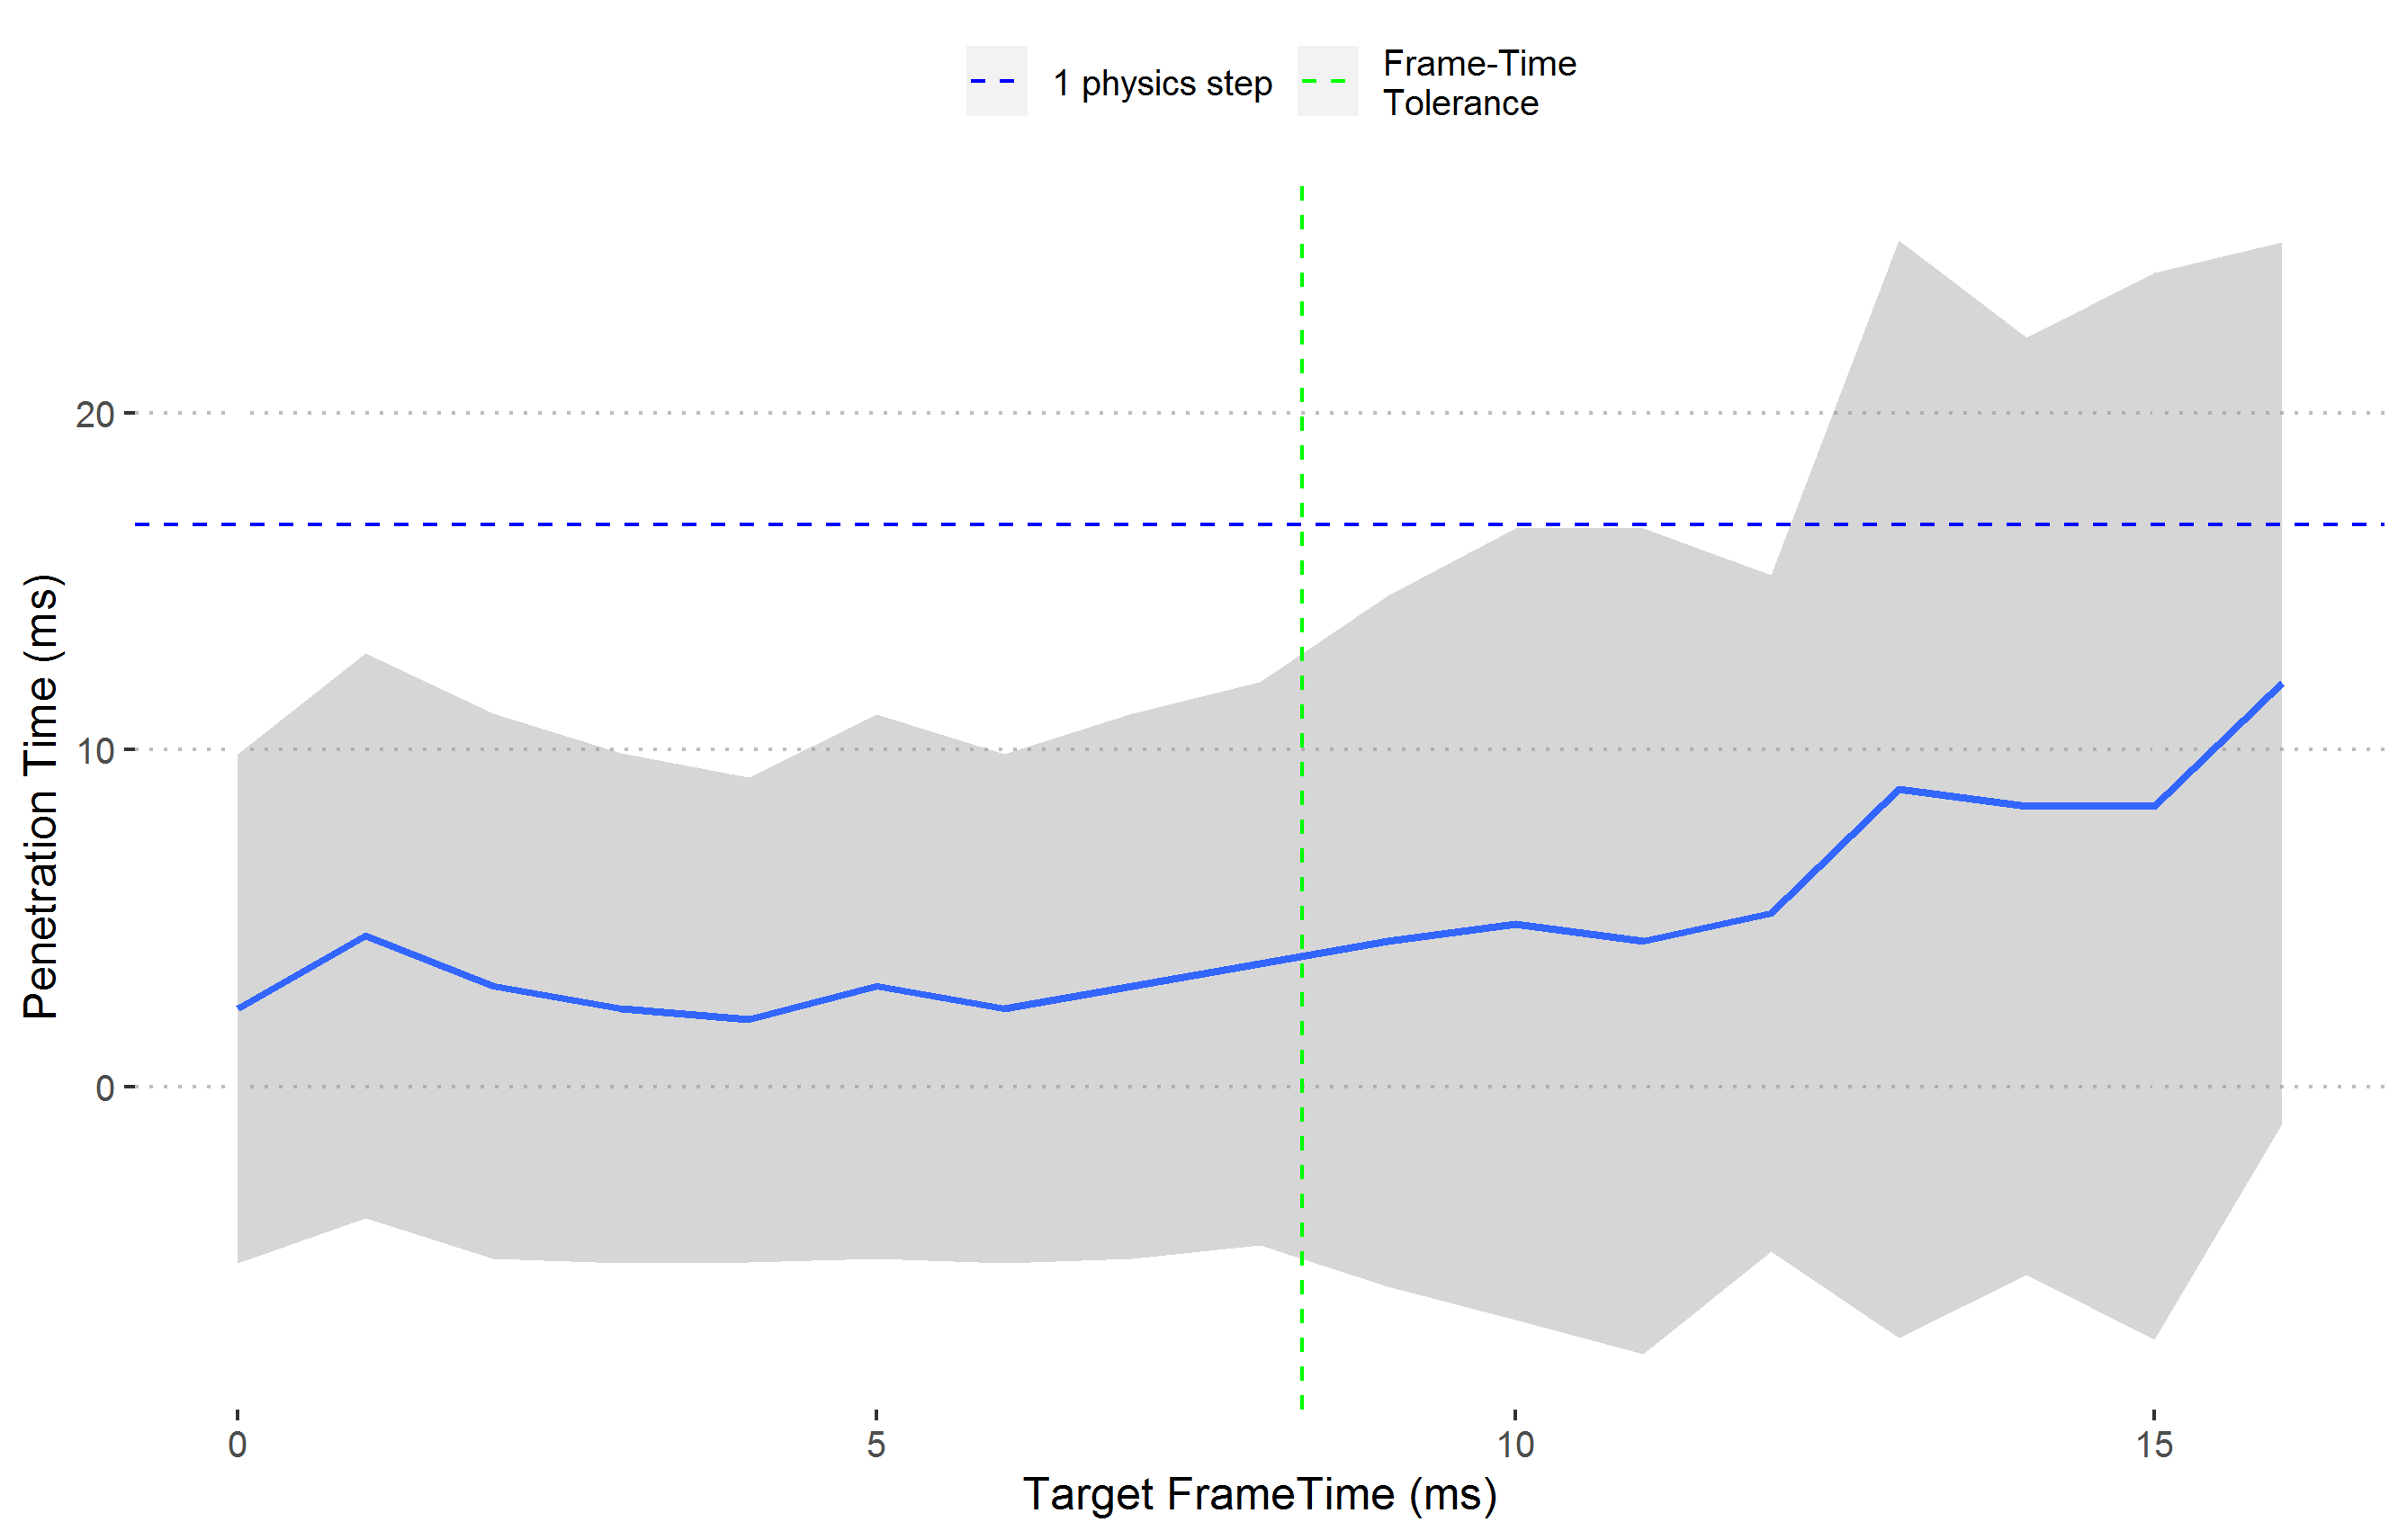
\includegraphics[width=\textwidth]{MeanPenVsFrameTimeLow}
	\caption{Mean penetration time of objects with $+/-2$ standard deviations with varying frame-time using a frame-time tolerance of $8ms$. The maximum expected penetration time of 1 physics step is marked with a dashed blue line. The frame-time tolerance is marked in a dashed green line.}
	\label{fig_CollisionsPenVsFrameTimeLow}
\end{figure}
\begin{figure}
	\centering
	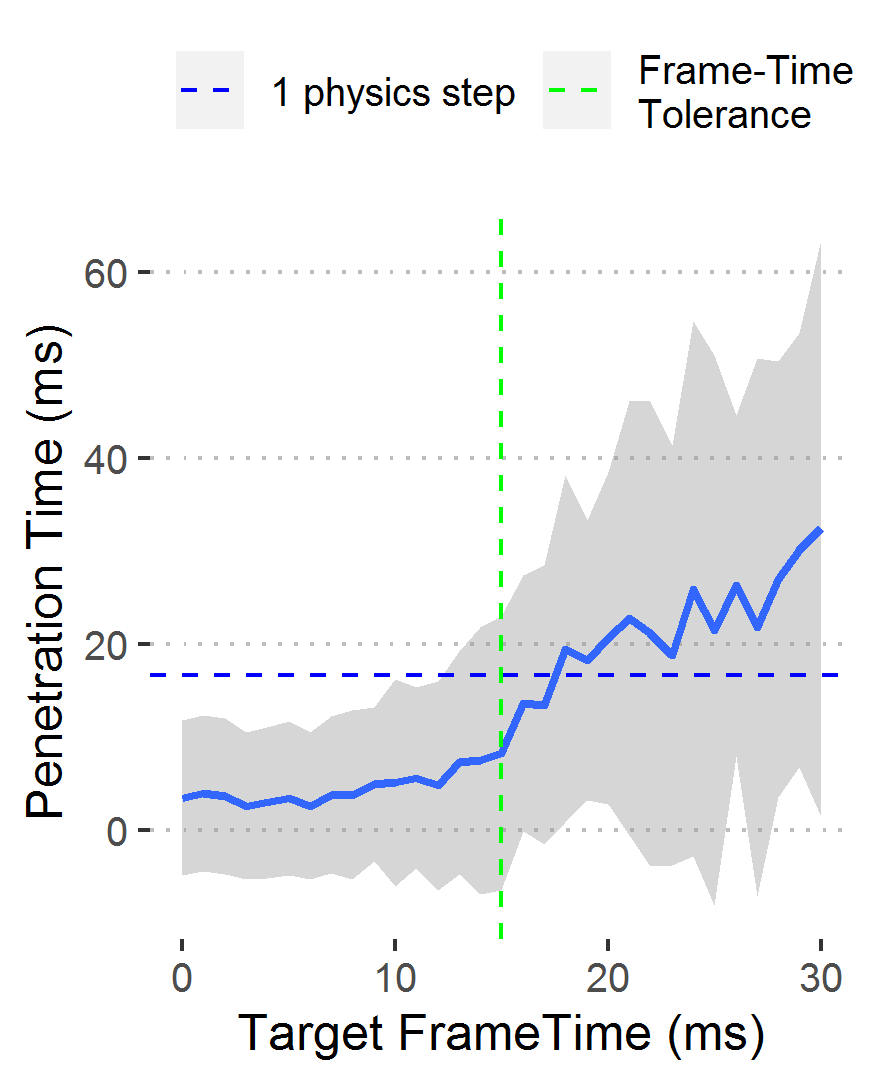
\includegraphics[width=\textwidth]{MeanPenVsFrameTimeMid}
	\caption{Mean penetration time of objects with $+/-2$ standard deviations with varying frame-time using a frame-time tolerance of $15ms$. The maximum expected penetration time of 1 physics step is marked with a dashed blue line. The frame-time tolerance is marked in a dashed green line.}
	\label{fig_CollisionsPenVsFrameTimeMid}
\end{figure}
\begin{figure}
	\centering
	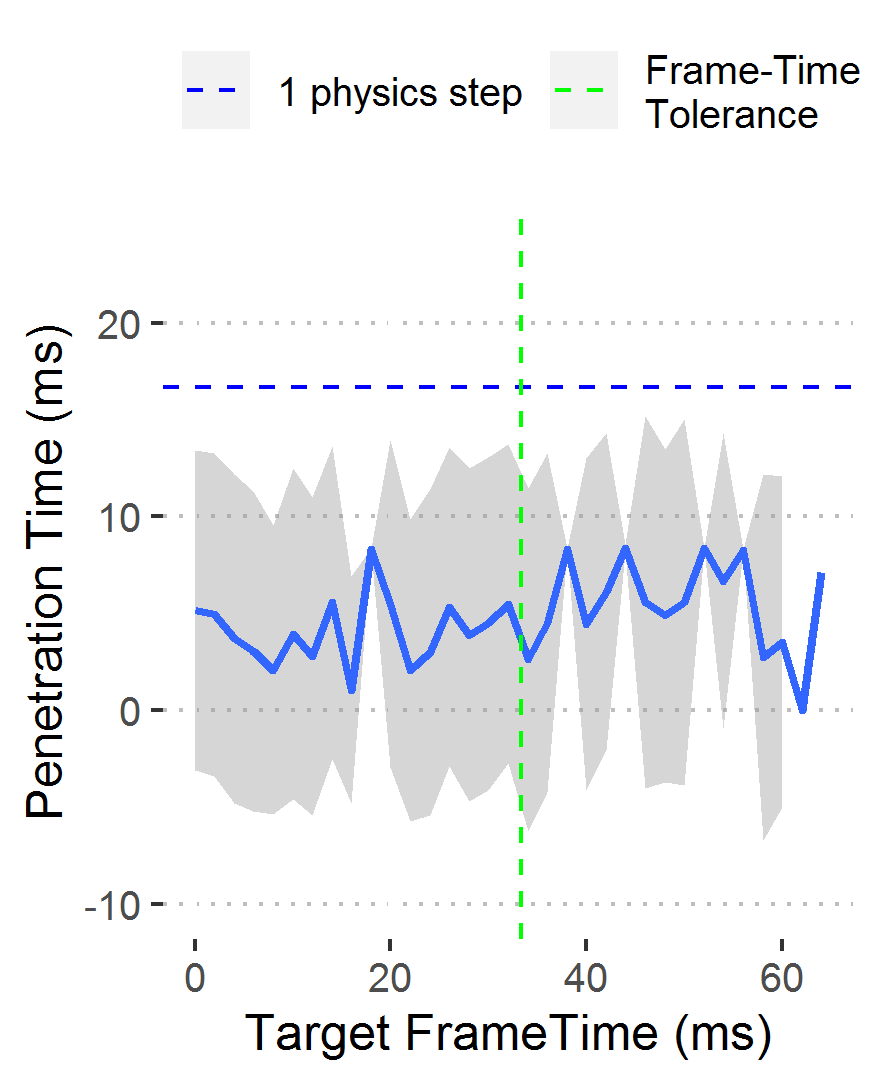
\includegraphics[width=\textwidth]{MeanPenVsFrameTimeHigh}
	\caption{Mean penetration time of objects with $+/-2$ standard deviations with varying frame-time using a frame-time tolerance of $32ms$. The maximum expected penetration time of 1 physics step is marked with a dashed blue line. The frame-time tolerance is marked in a dashed green line.}
	\label{fig_CollisionsPenVsFrameTimeHigh}
\end{figure}

%\begin{figure}
%\centering
%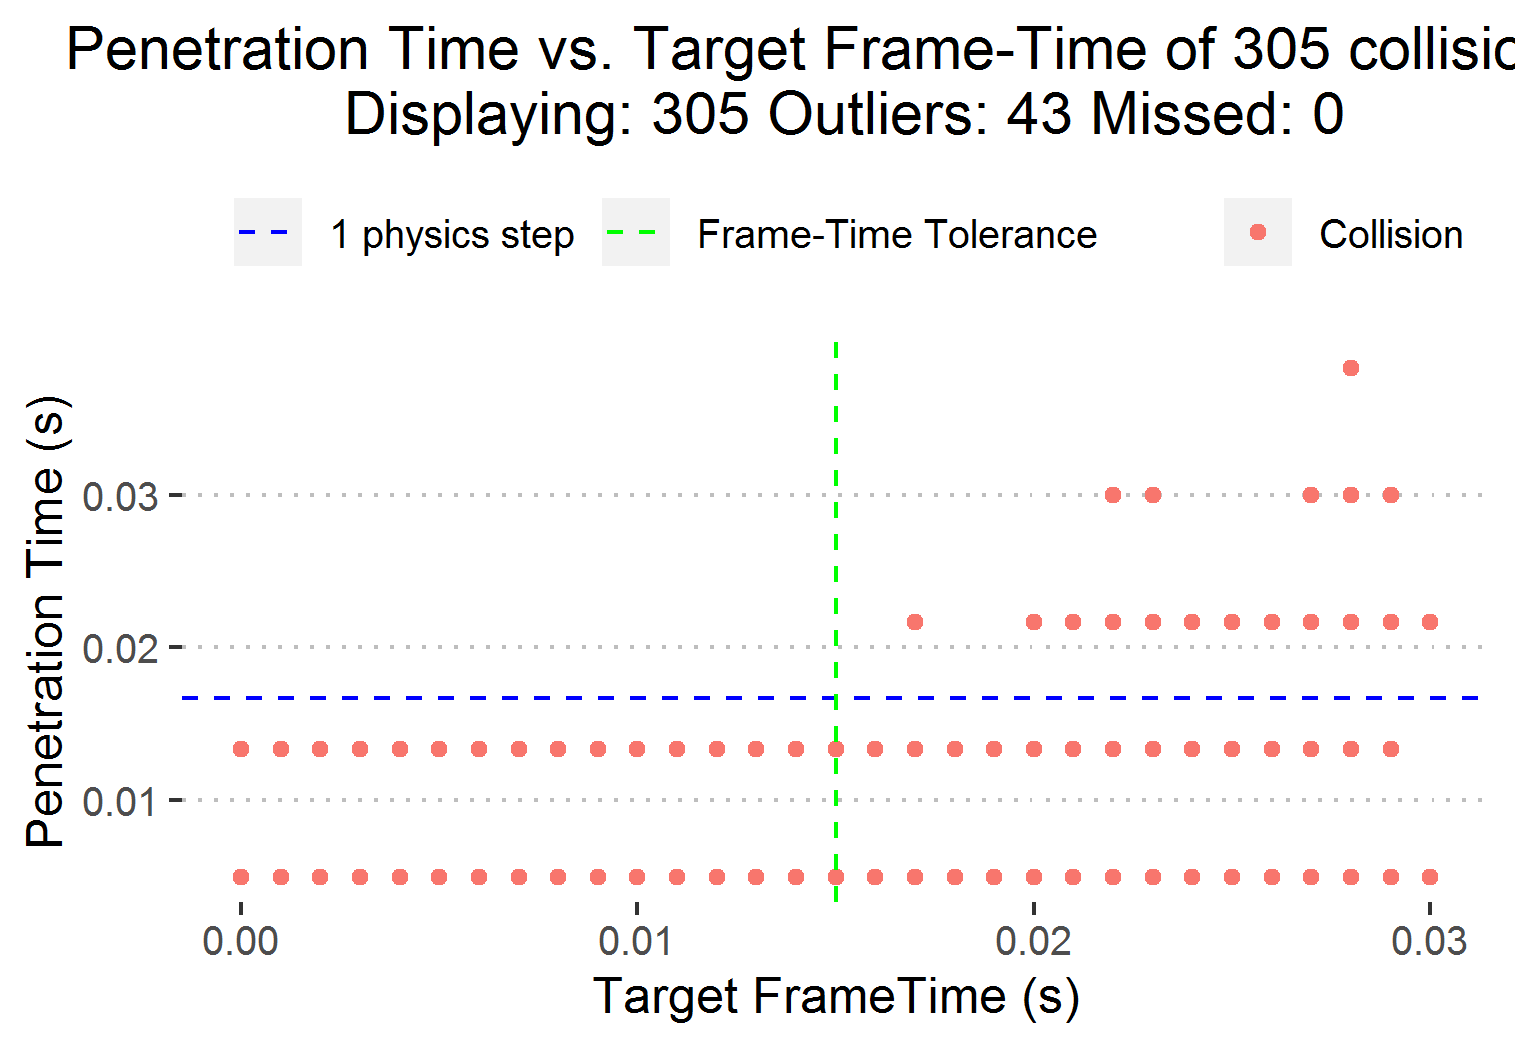
\includegraphics[width=\textwidth]{CollisionsPenVsFrameTime}
%\caption{Penetration time of objects with varying frame-time. Each red point represents one or more collisions. The maximum expected penetration time of 1 physics steps is marked with a dashed blue line. The speed tolerance is marked in a dashed green line. The number and magnitude of errors increases as target frame-time increases beyond the tolerance.}
%\label{fig_CollisionsPenVsFrameTime}
%\end{figure}
%
%\begin{figure}
%\centering
%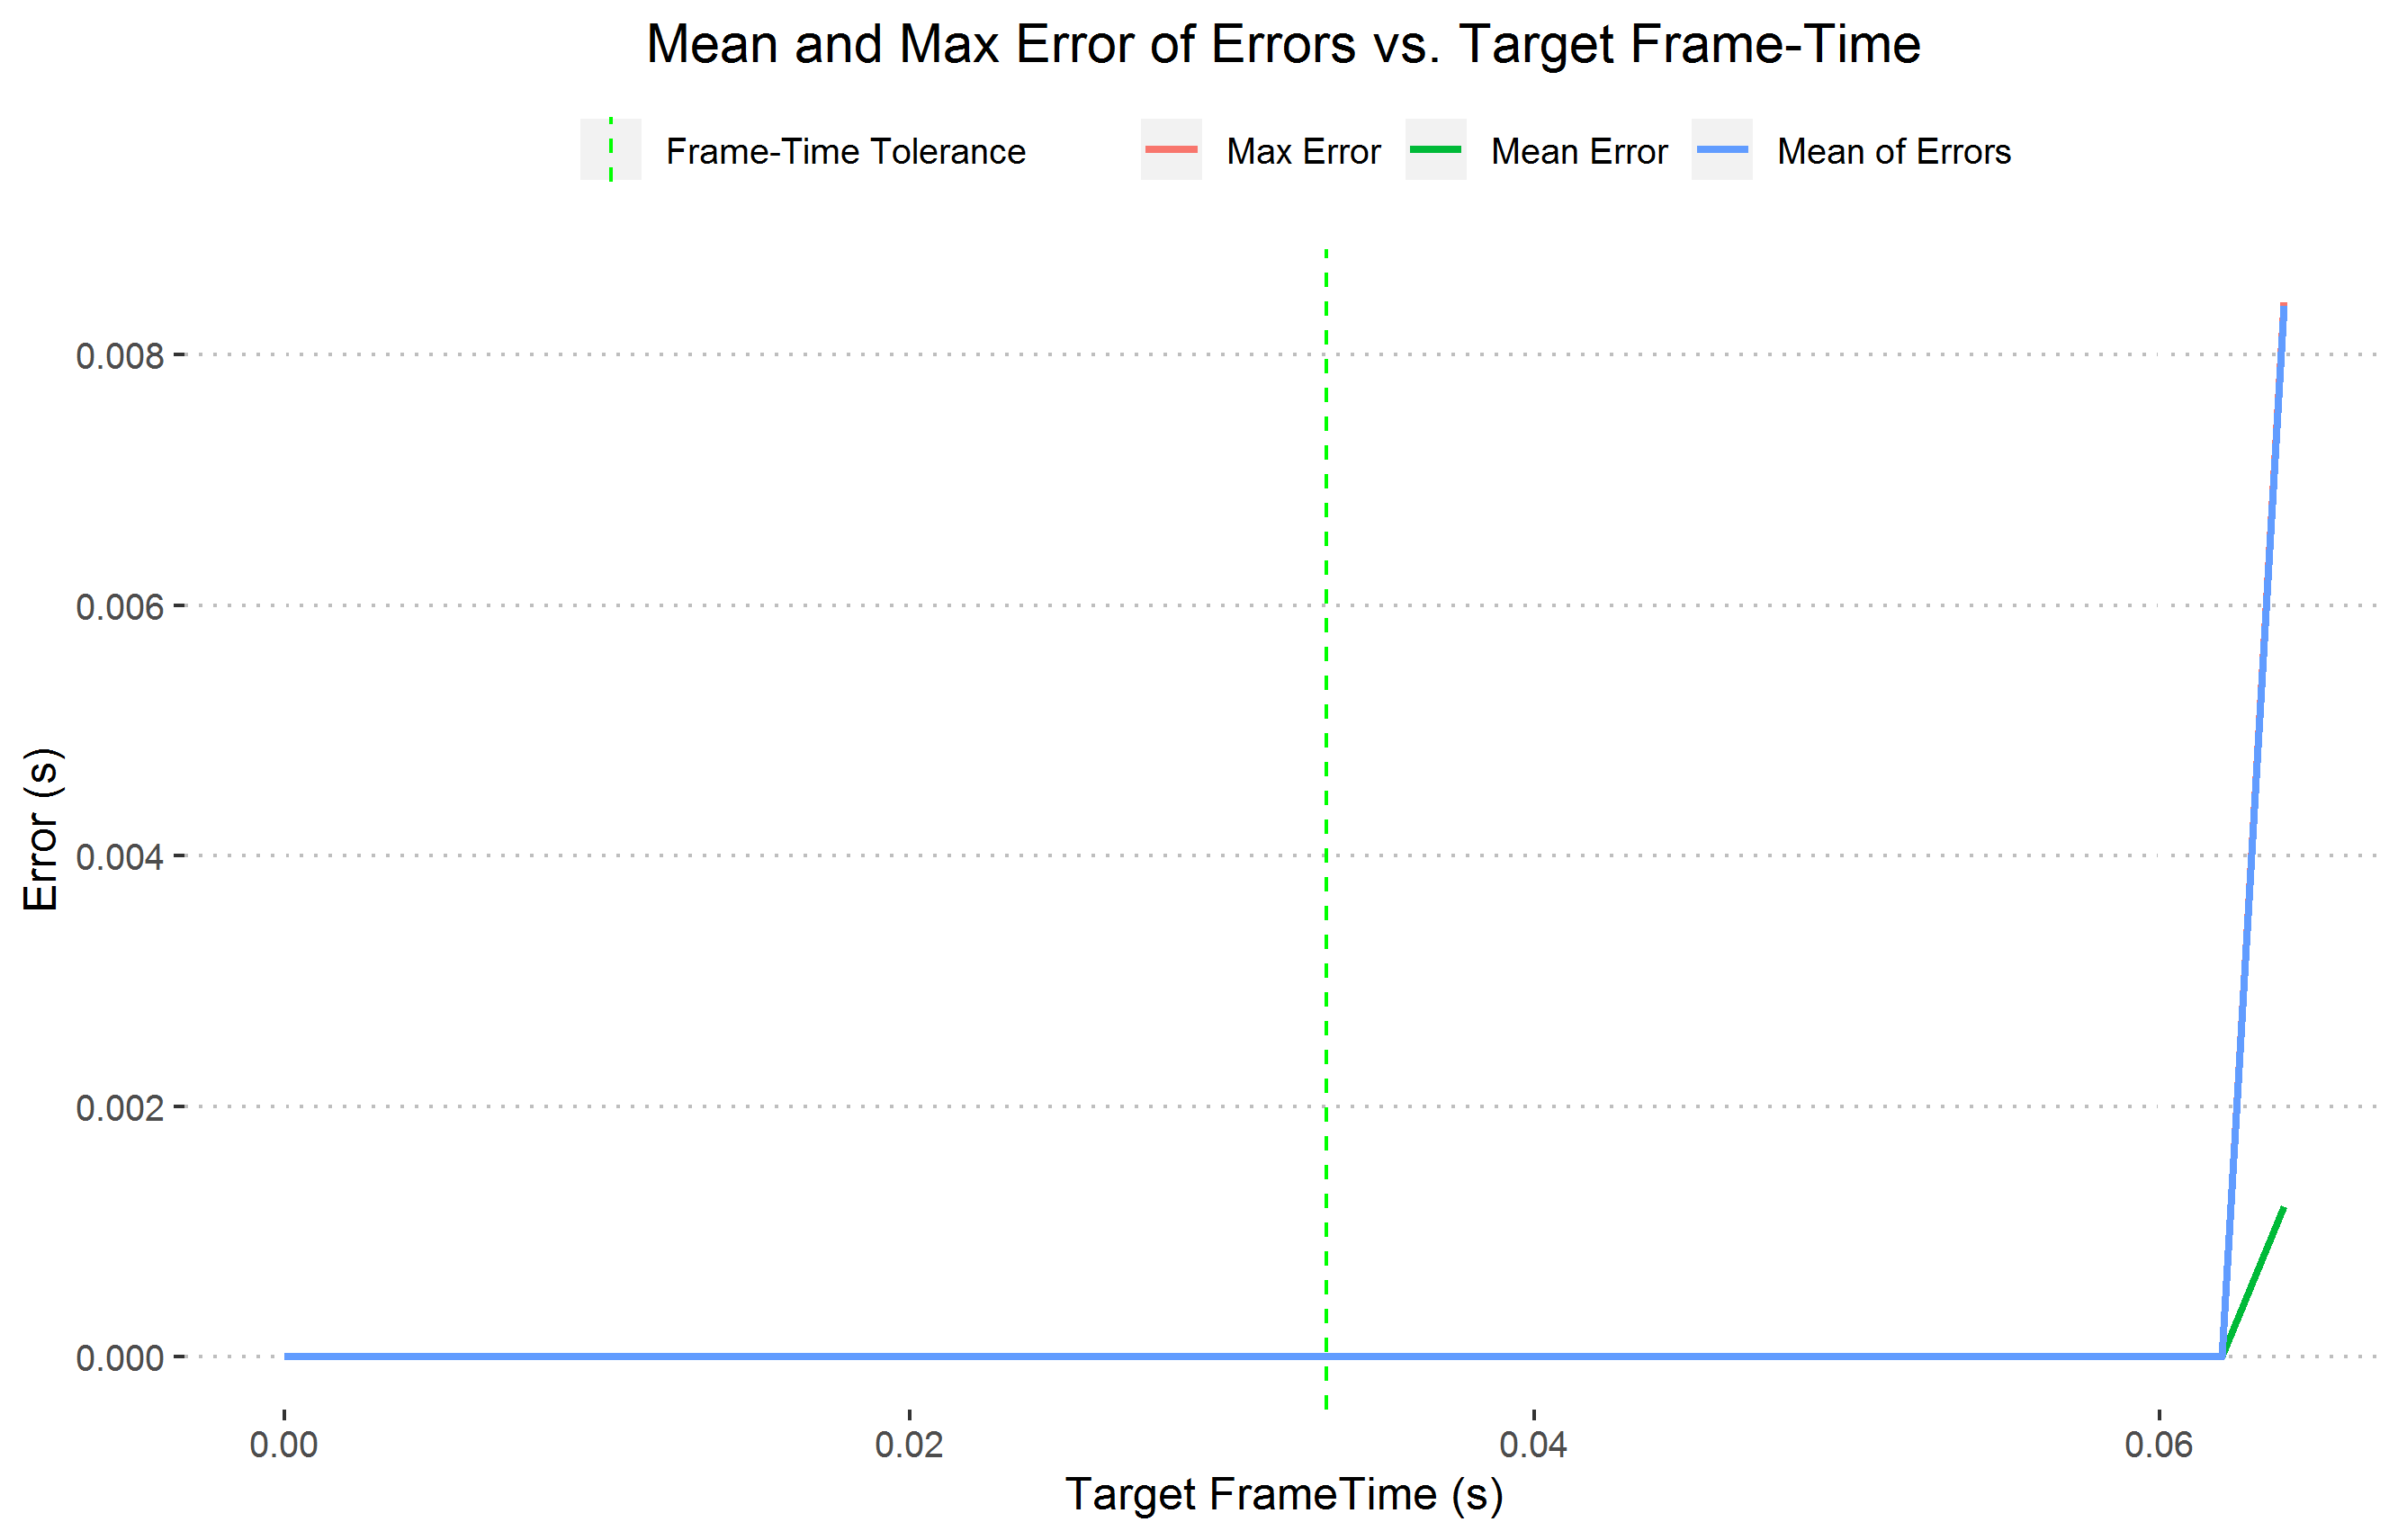
\includegraphics[width=\textwidth]{MeanMaxErrorVsFrameTime}
%\caption{The mean and max of collision errors with varying frame-time}
%\label{fig_MeanMaxErrorVsFrameTime}
%\end{figure}
%
%\begin{figure}
%\centering
%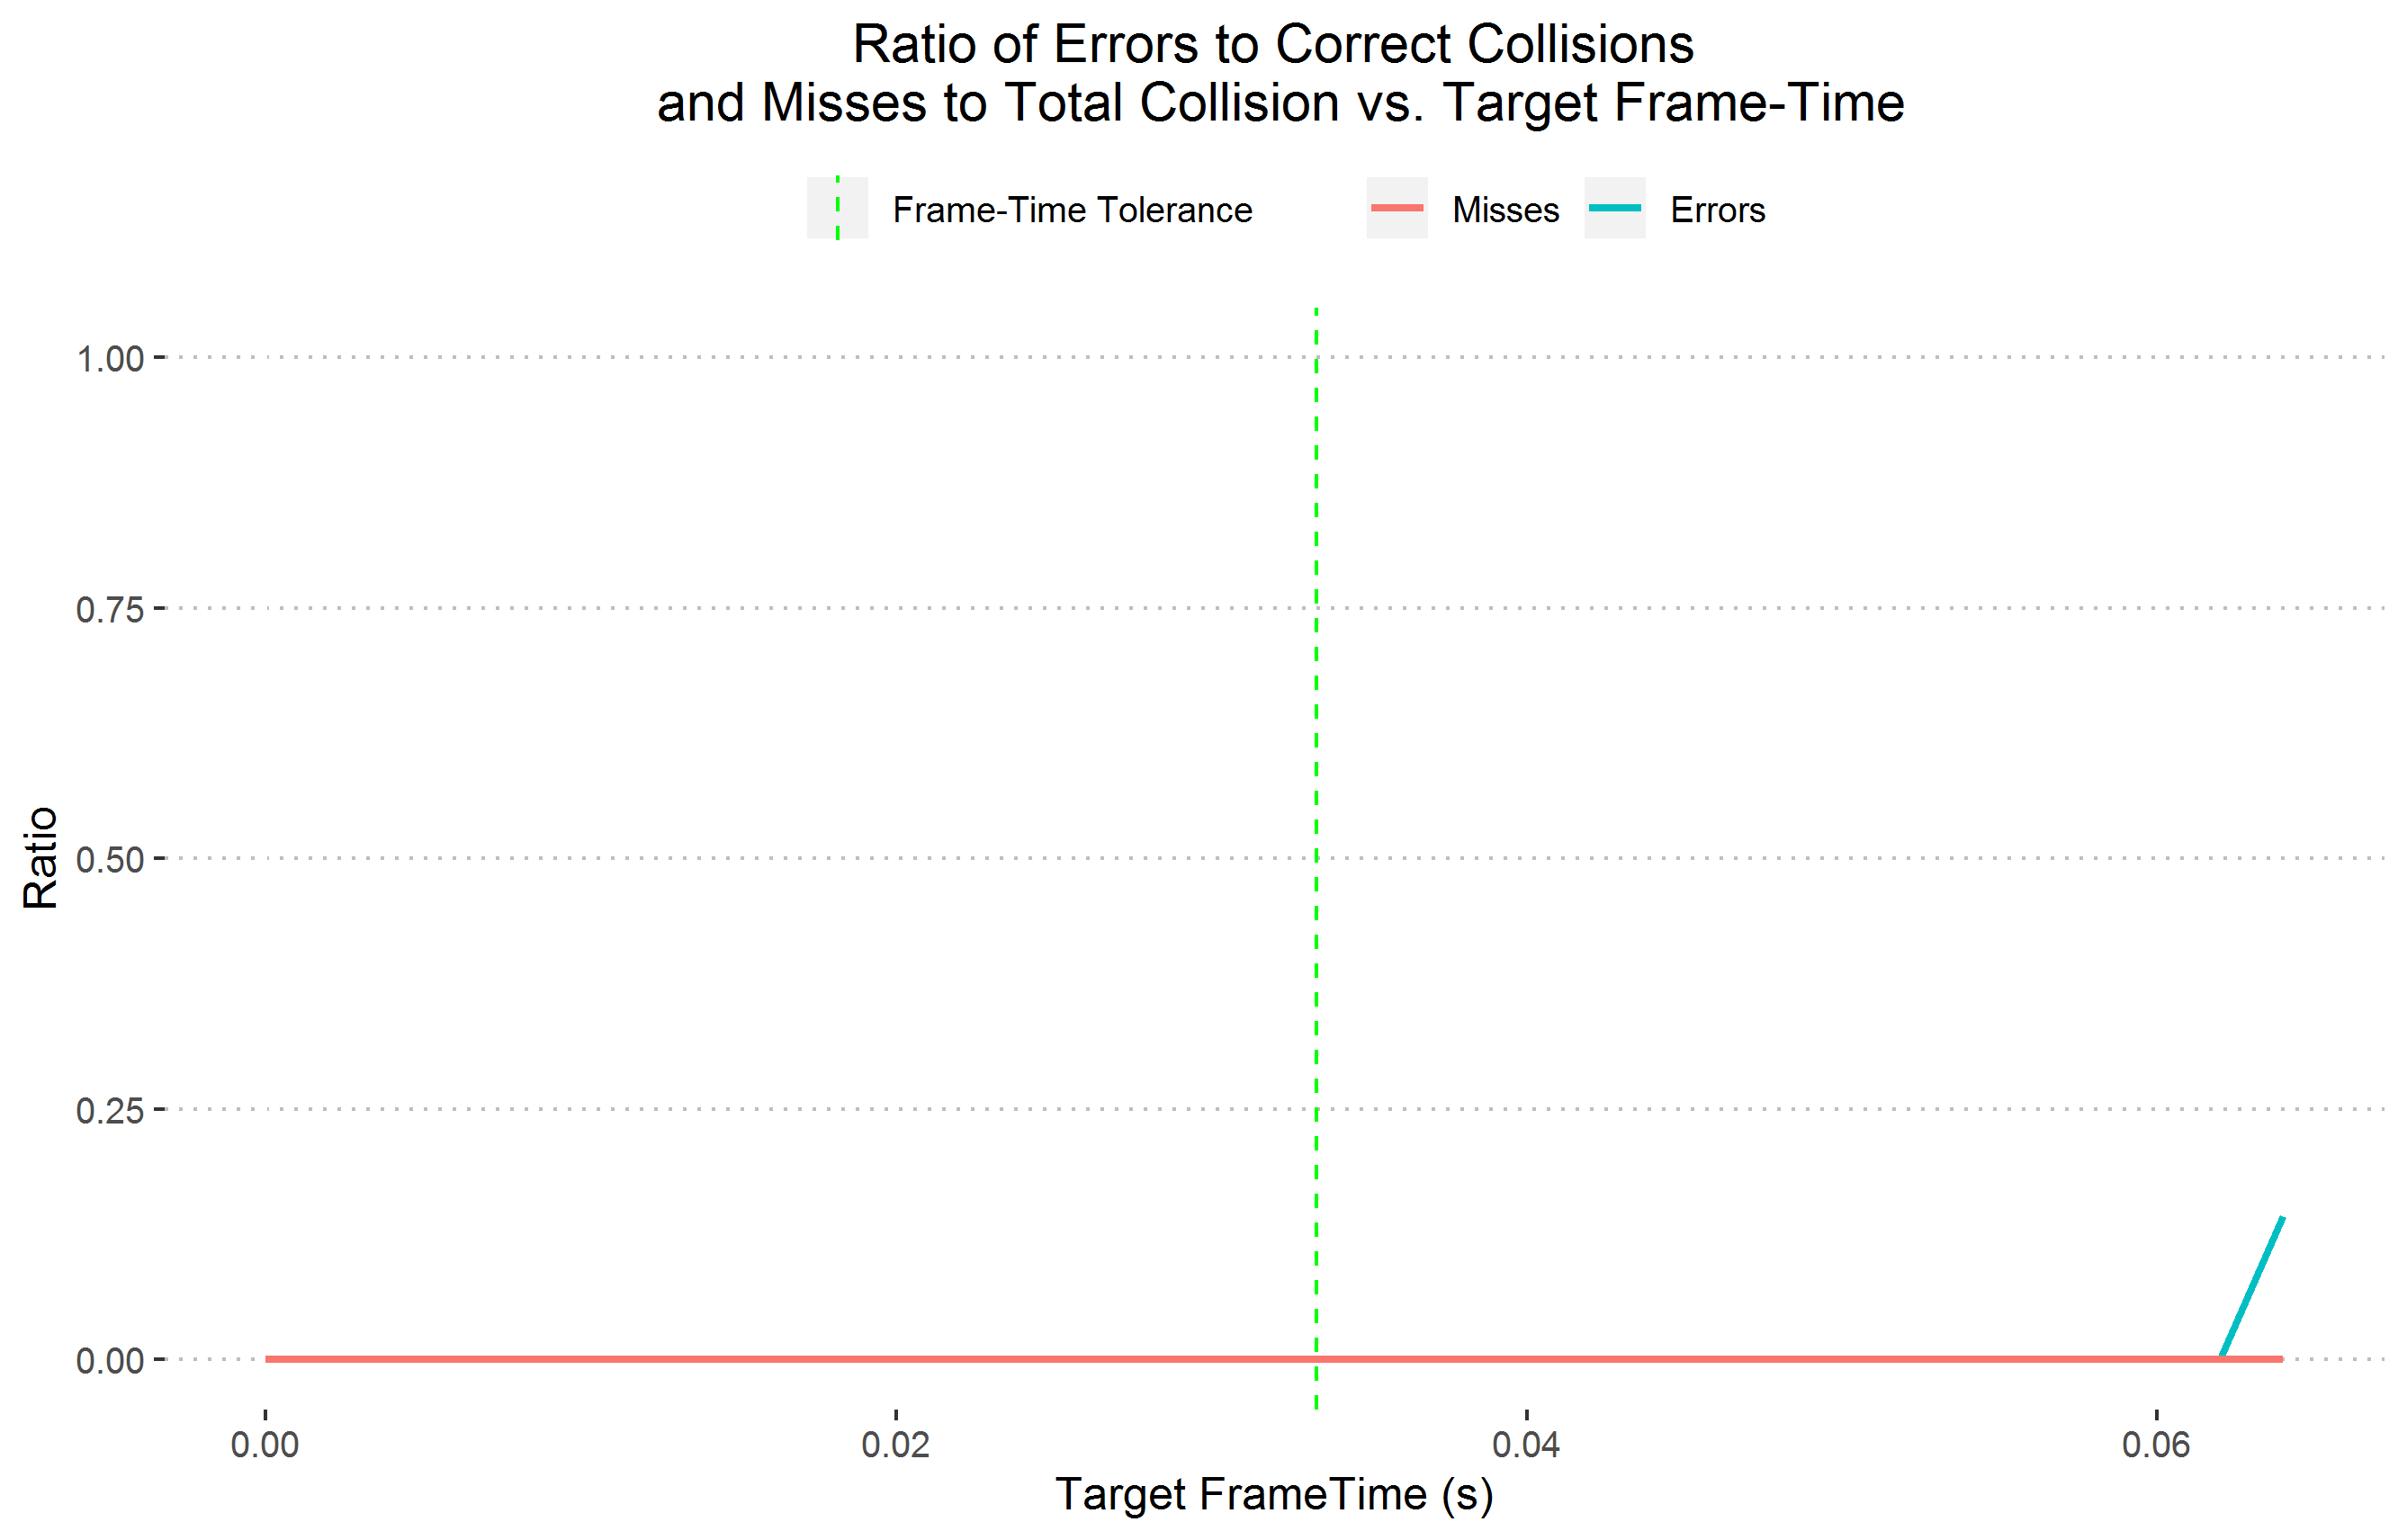
\includegraphics[width=\textwidth]{RatiosVsFrameTime}
%\caption{The ratios of erroneous collisions to correct collisions and missed collisions to total collisions with varying frame-time}
%\label{fig_RatiosVsFrameTime}
%\end{figure}

\begin{table}
	\centering
	\begin{tabular}{llrrrr}
		\toprule
		\multicolumn{1}{l}{Factor} & \multicolumn{1}{l}{Tolerance} & \multicolumn{1}{l}{N} & \multicolumn{1}{l}{Late \%} & \multicolumn{1}{l}{Miss \%} & \multicolumn{1}{l}{Thrashing}  \\ 
		\hline
		Speed      & 16m/s     & 800  & 1     & 0.13       &    0             \\
		Speed      & 32m/s     & 1600 & 0.688 & 0.0422     &    0             \\
		Speed      & 48m/s     & 2372  & 0.632& 0          &    28            \\
		Latency    & 2ms       & 1920  & 10.7 & 0          &    7             \\
		Latency    & 8ms       & 1520  & 0    & 0          &    30            \\
		Latency    & 16ms      & 797  & 2.50  & 0          &    53            \\
		Frame-Time & 8.33ms    & 450  & 0     & 0          &    0             \\
		Frame-Time & 15ms      & 800  & 1.88  & 0          &    0             \\
		Frame-Time & 33.33ms   & 251  & 0     & 0          &    523           \\
		\bottomrule
	\end{tabular}
	\caption{Results summary of collision correctness experiments before the tolerance was exceeded}
	\label{tab_BelowTolerance}
\end{table}

\begin{table}
	\centering
	\begin{tabular}{llrrrr}
		\toprule
		\multicolumn{1}{l}{Factor} & \multicolumn{1}{l}{Tolerance} & \multicolumn{1}{l}{N} & \multicolumn{1}{l}{Late \%} & \multicolumn{1}{l}{Miss \%} & \multicolumn{1}{l}{Thrashing}  \\ 
		\hline
		Speed      & 16m/s     & 800  &   49.9  & 0           & 0               \\
		Speed      & 32m/s     & 1589  &  48.6  & 0           & 11              \\
		Speed      & 48m/s     & 2233  &  45.10 & 1.12        & 167             \\
		Latency    & 2ms       & 1880  &  13.99 & 0           & 0               \\
		Latency    & 8ms       & 1377  &  0.15  & 0           & 121             \\
		Latency    & 16ms      & 574  &   12.20 & 0           & 226             \\
		Frame-Time & 8.33ms    & 400  &   9.50  & 0           & 0               \\
		Frame-Time & 15ms      & 750  &   58.13 & 0           & 0               \\
		Frame-Time & 33.33ms   & 106  &   1.89  & 0           & 693             \\
		\bottomrule
	\end{tabular}
	\caption{Results summary of collision correctness experiments after the tolerance was exceeded}
	\label{tab_AboveTolerance}
\end{table}

\subsubsection{Thrashing}
In addition to recording the number of collisions that resulted in thrashing, the number of times an object thrashed between servers was also measured. The number of times thrashed is determined by measuring the number of migrations away from the server that the collisions takes place on, before the collision takes place. A histogram of the number of occurrences against the number of times thrashed is shown in Fig. \ref{fig_ThrashingHistogram}. For this histogram, data from the Frame-Time $33.33ms$ experiment is used, as this provides the largest sample of thrashing. Fig. \ref{fig_ThrashingHistogram} demonstrates that the most frequent number of times thrashed is 1, by a large margin followed by a downward trend.

The more times thrashing occurs, the later the collision may be detected as objects continue to be updated and move without a collision occurring. It should be noted that thrashing occurring does not guarantee that a late collision will take place. The more times thrashing takes place, the more physics updates occur and the further the objects may be moved towards (and eventually overlapping) each other. Therefore, a greater number of times thrashed, means a late and incorrect collision response is more likely, but not guaranteed.

\begin{figure}[t]
	\centering
	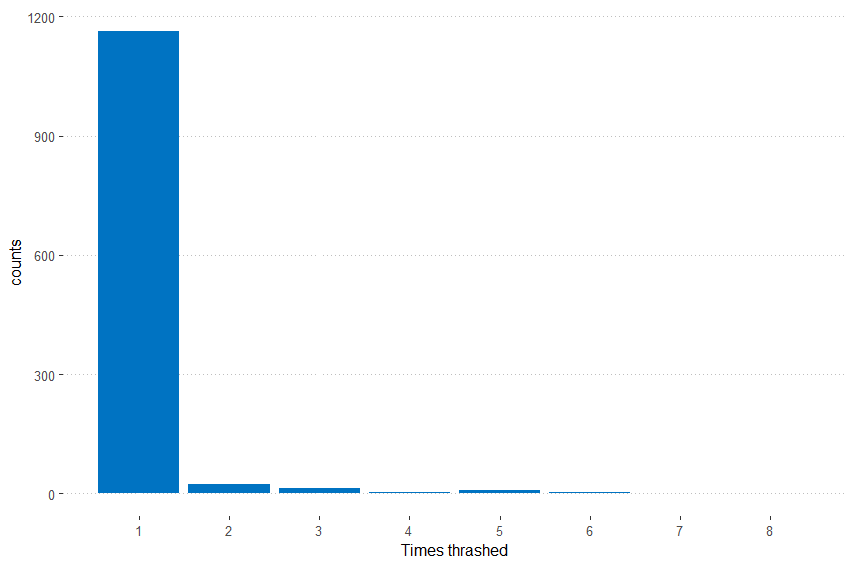
\includegraphics[width=\textwidth]{ThrashingHistogram}
	\caption{Thrashing Histogram. The number of occurrences vs the number of times thrashed.}
	\label{fig_ThrashingHistogram}
\end{figure}

\subsubsection{Evaluation - Speed}
As the speed increases, the proportion of late collisions to correct collisions increases, as shown in Figs. \ref{fig_RatioVsSpeedLow}, \ref{fig_RatioVsSpeedMid} and \ref{fig_RatioVsSpeedHigh}. When speed is below the speed tolerance, late collisions do not exceed 10\%. This 10\% is assumed to be caused by false-positives. Once above the speed tolerance, the proportion of late collisions increases immediately, which is predicted by the aura calculation. Missed collisions begin to occur when speed exceed $80ms^{-1}$ in the $48ms^{-1}$ experiment, this is due to objects travelling so quickly, the objects completely pass one another, missing the collision entirely.

It should also be noted that object speed is application specific and objects need to be travelling directly towards the centre of each other and one of the objects has to be travelling above the tolerance speed, in order for errors to occur.

As the speed increases, the mean penetration time increases, as shown in Figs. \ref{fig_CollisionsPenVsSpeedLow}, \ref{fig_CollisionsPenVsSpeedMid} and \ref{fig_CollisionsPenVsSpeedHigh}. With the exception of the starting speed, the standard deviation remains constant below the tolerance line. Once speed increases above the tolerance line, the standard deviation initially increases, but appears to remain constant after the initial increase. 
%Note that the mean error increases in discrete steps (with some small variation), this is due to the discrete physics time-steps.

\subsubsection{Evaluation - Latency}
As the latency increases, the proportion of late collisions to correct collisions increases, as shown in Fig. \ref{fig_RatioVsLatencyHigh}. However, Figs. \ref{fig_RatioVsLatencyLow} and \ref{fig_RatioVsLatencyLow} do not show this relationship. In the $2ms$ latency tolerance experiment, late collisions do not exceed $20\%$, which is assumed to be accounted for by false-positives. The aura calculation predicts that late collisions should start occurring once $3ms$ has been exceeded, however, this is not observed, as the proportion does not increase above what would be expected for false-positives.
In the $8ms$ latency tolerance experiment, late collisions do not exceed $2\%$, which is assumed to be accounted for by false-positives. This remains the case even when the tolerance is exceeded. The aura calculation predicts that late collisions will not begin to occur until $20ms$ latency is reached, which this experiment does not reach, therefore no late collisions outside of false-positives are expected. In the $16ms$ latency tolerance experiment, late collisions do not exceed $3\%$ below the tolerance, which is assumed to be accounted for by false-positives. The aura calculation predicts that late collisions will not begin to occur until $20ms$ latency is reached. In Fig. \ref{fig_RatioVsLatencyHigh} we see the proportion of errors increase from $20ms$ and above, however, it does not exceed the expected false-positive proportion until $25ms$ latency is reached.
%TODO: Re-run latency experiment, larger sample size?

%When latency is below the latency tolerance, late collisions do not exceed 10\%. This 10\% can be accounted for by false-positives. Once above the speed tolerance, the proportion of late collisions increases immediately, which is predicted by the aura calculation.

As latency increases standard deviation remains constant below the tolerance value, as shown in Figs. \ref{fig_CollisionsPenVsLatencyLow}, \ref{fig_CollisionsPenVsLatencyMid} and \ref{fig_CollisionsPenVsLatencyHigh}. With only a small number of exceptions (in $2ms$ experiment), the mean $+2$ standard deviations does not exceed the maximum expected penetration when below the latency tolerance. Above the latency tolerance value, the standard deviation increases for the $16ms$ tolerance experiment, but remains constant for the first two latency experiments. In addition, the first two experiments do not show a clear increase in mean penetration, this is due to the aura calculation's discrete nature and as $15ms$ has been used for the frame-time tolerance, small increases in latency of $2$ and $8ms$ will not show the increase in error to the next discrete step. However, in the final experiment using $16ms$, the relationship of increasing penetration as latency increases is demonstrated.

The $2ms$ latency tolerance experiment exhibits more false-positives than the other experiments, including across the entire range of values used. This may be a result of small aura sizes producing more false-positive, the sample size being to small or another unknown effect which has not been accounted for. In addition, although late collisions increase as actual latency exceeds $20ms$ in the $15ms$ tolerance experiment, the mean $+2$ standard deviations does not exceed the maximum expected penetration line until $26ms$ actual latency is reached. Both of these unexpected results should be investigated further in the future.

Outside of cloud-server to cloud-server communication latency is prone to ``jitter'', meaning tolerances are likely to be sometime exceeded, however, ``jitter'' is for short durations and would need to take place at the same time as an object migration. However, cloud-server to cloud-server communication has negligible ``jitter'' \cite{ThousandEyesCloudPerf2018}. If collision correctness is required even in cases of ``jitter'', the latency tolerance would need to be higher than the peaks in latency. 

\subsubsection{Evaluation - Frame-Time}
As frame-time increases, the proportion of late collisions to correct collisions increases, as shown in Figs. \ref{fig_RatioVsLatencyLow} and \ref{fig_RatioVsLatencyMid}, however in \ref{fig_RatioVsLatencyHigh} the sample size is small above the tolerance line due to the high occurrences of thrashing and so the relationship in this experiment can not be deduced. For the $8ms$ and $15ms$ experiments the late collisions do not exceed 10\% and are assumed to be accounted for by false-positives. In the $8ms$ frame-time tolerance experiment, late collisions are not expected to occur until $16ms$ frame-time, based on the aura size. Late collisions do not exceed $20\%$ and is assumed to be accounted for by false-positives. In the $15ms$ frame-time tolerance experiment, late collisions exceed $20\%$ once $16ms$ latency is exceeded as predicted by the aura size and increase to over $75\%$ at $30ms$ latency.
In the final frame-time tolerance experiment using $32ms$ frame-time tolerance, late collisions only occur for frame-times of $64ms$. The aura calculation predicts that late collisions should begin to occur as soon as $32ms$ frame-time is exceeded, however, due to the low sample size, as a result of the high occurrences of thrashing, the plot does not accurately represent any relationship between frame-time and proportion of late collisions.

For the first two frame-time experiments ($8.33ms$ and $15ms$ tolerance values), as frame-time increases, the mean penetration time increases and standard deviation also increases, shown in Figs. \ref{fig_CollisionsPenVsFrameTimeLow} and \ref{fig_CollisionsPenVsFrameTimeMid}. Standard deviation increases as the delay between frame-time update and physics update can always vary between 0 and the frame-time, meaning even in high frame-time situations, the delay between frame-time update and physics update can be 0. Exceeding the frame-time tolerance very quickly leads to high max error. This is due to the delay in messages being exchanged being created by the long frame-times on both servers (this is reflected in the aura calculation by the frame-time tolerance being multiplied by 2). However, as the target frame-time increases over the tolerance, variation in error increases and maximum errors become less likely. For the final frame-time experiment, ($33.33ms$ tolerance value), thrashing occurs the majority of the time (as demonstrated in \ref{tab_BelowTolerance} and \ref{tab_AboveTolerance}), both above and below the tolerance, due to this the results shown in \ref{fig_CollisionsPenVsFrameTimeHigh} have a very small sample size and thus will not accurately represent the relationship between frame-time and penetration.

\subsubsection{Varying Factors - Summary}
The varying factors experiments demonstrate that the aura calculation is conclusively correct for speed and frame-time aura tolerance factors and at minimum approximate for latency. For each varied factor, for all three tolerance values chosen, below the tolerance value, the mean + two standard deviations lies under the maximum penetration time expected on a centralised simulation, with only a small number of exceptions discussed above. These experiments also demonstrate the relationship between increasing the tolerance values and amount of thrashing expected to occur. There are no missed collisions, with the exception of the speed experiments and these have significantly fewer than $1\%$ misses below the tolerance and $1.12\%$ misses above the tolerance. Once factors increase above their respective tolerance values, late collisions begin to occur and the more the factors are exceeded, the number and magnitude of errors increase. This demonstrates the correctness of the aura calculation in AP.
%Therefore, we have shown that if the aura calculation factors remain within their respective tolerances, erroneous collisions will be small in magnitude and rare in number. %TODO: Summary Table: Row for each factor: Number of collisions below tolerance, Percentage of errors below tolerance, Mean error below tolerance

%TODO: The following needs to be formalised.

%The varying factors experiments demonstrate that the aura calculation is either correct or close to correct for all aura tolerance factors. For each varied factor below the tolerance value there are only a small number of erroneous collisions just below the tolerance value and no missed collisions. Once factors increase above the tolerance value erroneous collisions begin to occur with increasing number and magnitude.

%If the aura calculation factors remain within their respective tolerances, erroneous collisions will be small in magnitude and rare in number. %TODO: Summary Table: Row for each factor: Number of collisions below tolerance, Percentage of errors below tolerance, Mean error below tolerance

%Which factors lead to greatest:
%Ratio of errors - Relative Speed 90%+ >110m/s
%Magnitude of errors (overall) - Relative Speed
%Magnitude of errors (just errors) - Relative Speed
%Max Error - Relative Speed


%TODO: Talk about how errors increase with each factor
%TODO: Check for small numbers of errors below tolerances
%There are no erroneous collisions below the tolerance apart from in the latency experiment, but I was expecting a small number of errors below the tolerance lines due to the way the frame-time control works

\subsection{Experiment - Varying Packet-Loss}

In addition to varying each aura tolerance factor, an experiment was undertaken to determine the effects of packet-loss on the correctness of collisions between objects. In this experiment the packet-loss was varied from $0\%$ to $20\%$ in increments of $1\%$. The aura calculation does not account for packet-loss and and therefore there is no aura tolerance. Packet-loss is controlled using the Traffic Control tool; it is simulated on each server for all communication received from the other server.

RakNet, the library used for network communication in this project, includes a reliability layer, which uses best effort. This means if packets are lost and an acknowledgement message is not received, sending will be re-attempted, but message delivery cannot be guaranteed. However, this takes time and therefore causes a delay in messages being received. Delays in messages will lead to erroneous collisions, therefore as packet-loss increases, erroneous collisions should increase in number and magnitude. If messages are delayed enough, the collision will be missed as the two objects pass each other on different servers without ever interacting with each other. 

\subsubsection{Experiment parameters and output}
The two servers use the following tolerances: a maximum speed tolerance of $32m\mathord{\cdot}s^{-1}$; maximum latency tolerance of $2ms$; and a maximum frame-time tolerance of $15ms$. Each server has a random delay before starting between $0$ and the target frame-time in order to prevent the two servers always having synchronous update cycles. Each experiment is repeated $50$ times. The mean and $+/-2$ standard deviations of penetration time were plotted against each tolerance factor for each of the three tolerance values chosen. In addition, the ratio of errors to correct collisions and misses to total collisions were plotted against packet-loss.

\begin{figure}
	\centering
	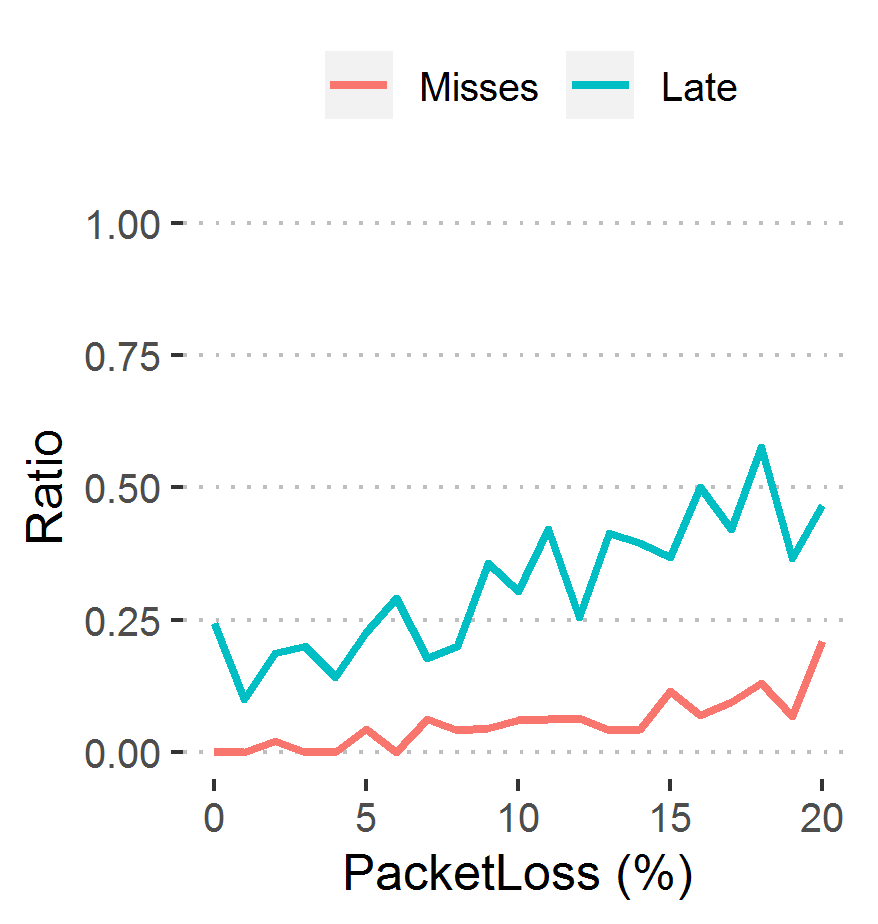
\includegraphics[width=\textwidth]{RatiosVsLoss}
	\caption{The ratios of erroneous collisions to correct collisions and missed collisions to total collisions with varying packet loss.} %As packet-loss increases from $10\%$ to $20\%$ the ratio of erroneous collisions to correct collisions sharply increases as does misses to total collisions. Above $60\%$ packet-loss, all collisions are missed.}
	\label{fig_RatiosVsLoss}
\end{figure}

\begin{figure}
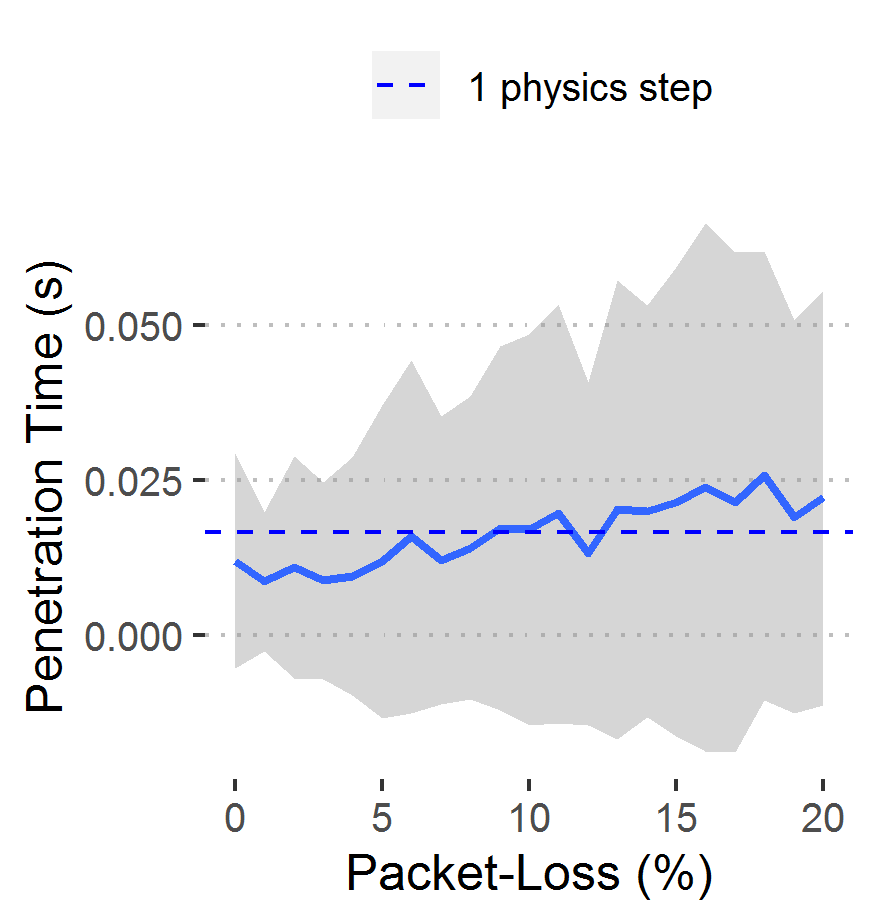
\includegraphics[width=\textwidth]{MeanPenVsLoss}
\caption{Mean penetration time of objects with $+/-2$ standard deviations with varying packet-loss. The maximum expected penetration time of 1 physics steps is marked with a dashed blue line.}
%\caption{Penetration time of objects with varying packet-loss. Each red point represents one or more collisions. The maximum expected penetration time of 1 physics steps is marked with a dashed blue line. The number and magnitude of errors increases as packet-loss increases beyond $10\%$.}
\label{fig_CollisionsPenVsLoss}
\end{figure}

%In addition to varying each aura tolerance factor, an experiment was also carried out to determine the effects of packet-loss on the correctness of collisions between objects. In this experiment the packet-loss was varied from $0\%$ to $80\%$ in increments of $10\%$. Packet-loss is not factored into the aura calculation and therefore has no tolerance. Packet-loss is controlled using the Traffic Control tool; packet-loss is emulated on each server for all communication received from the other server.
%
%RakNet, the library used for network communication in this project, includes a reliability layer. This means if packets are lost and an acknowledgement message is not received, sending will be re-attempted. However, this takes time and therefore causes a delay in messages being received. Delays in messages will lead to erroneous collisions, therefore as packet-loss increases, erroneous collisions should increase in number and magnitude. If messages are delayed enough, the collision will be missed as the two objects pass each other on different servers without ever interacting with each other. 
%
%%TODO: Check if aura updates are ordered, mention that here.
%%RakNet's reliability layer uses best effort, meaning messages are not guaranteed to be received, which means some messages may never be received resulting in 
%
%\begin{figure}
%\centering
%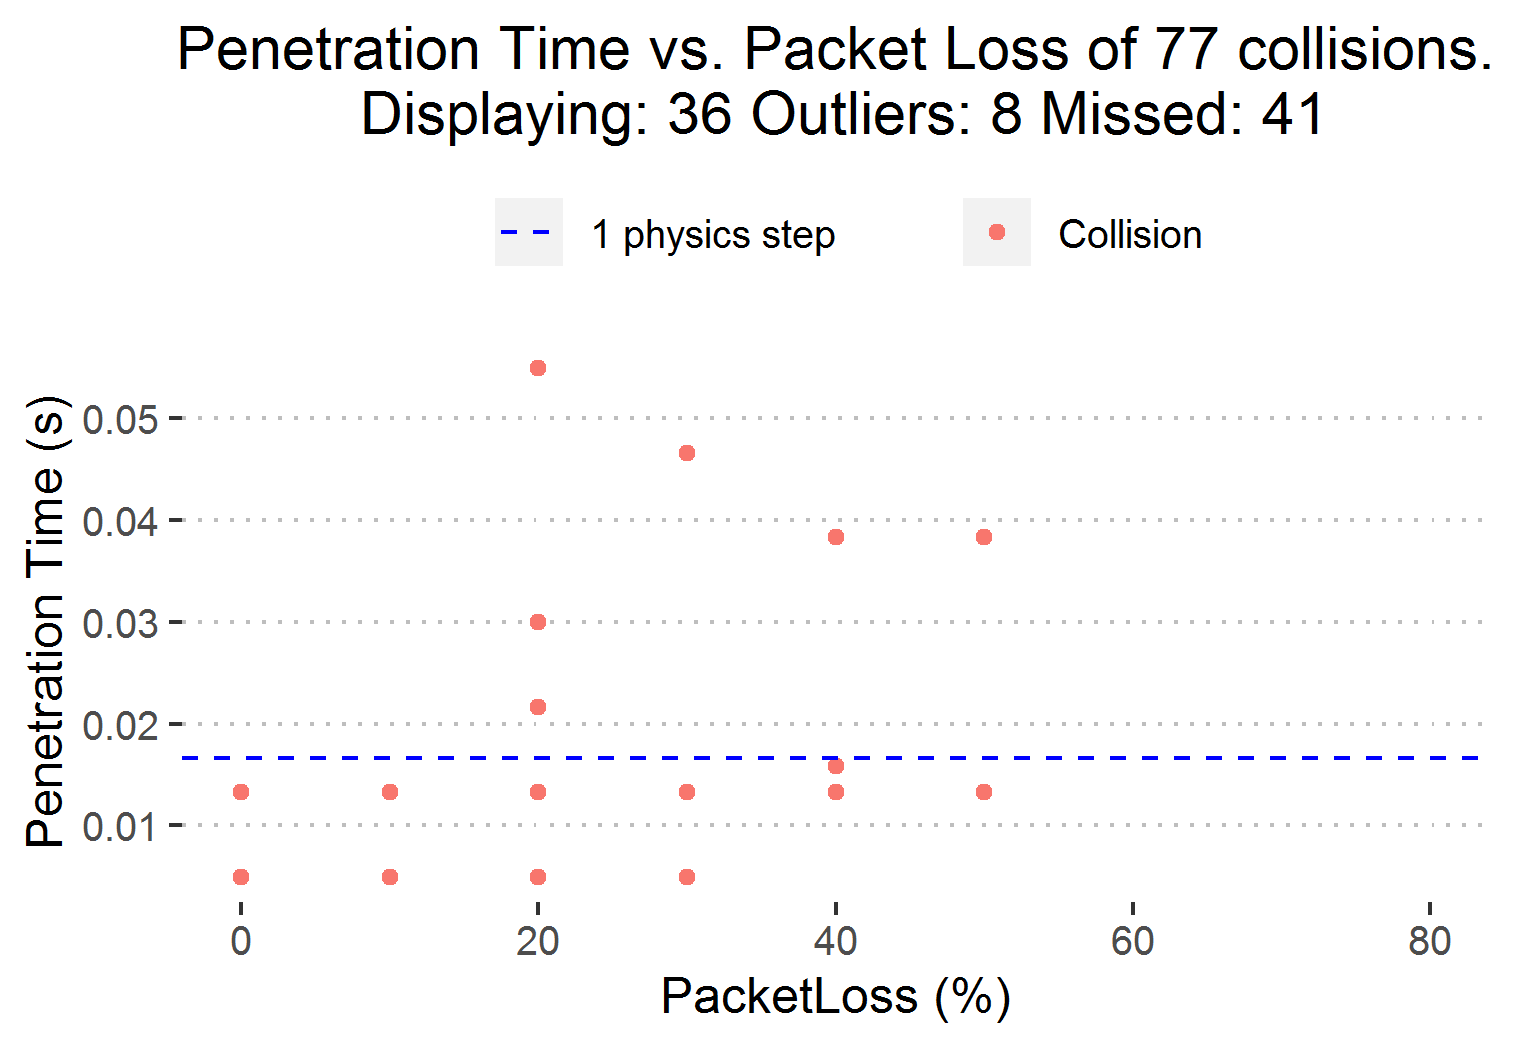
\includegraphics[width=\textwidth]{CollisionsPenVsLoss}
%\caption{Penetration time of objects with varying packet-loss. Each red point represents one or more collisions. The maximum expected penetration time of 1 physics steps is marked with a dashed blue line. The number and magnitude of errors increases as packet-loss increases beyond $10\%$.}
%\label{fig_CollisionsPenVsLoss}
%\end{figure}
%
%\begin{figure}
%\centering
%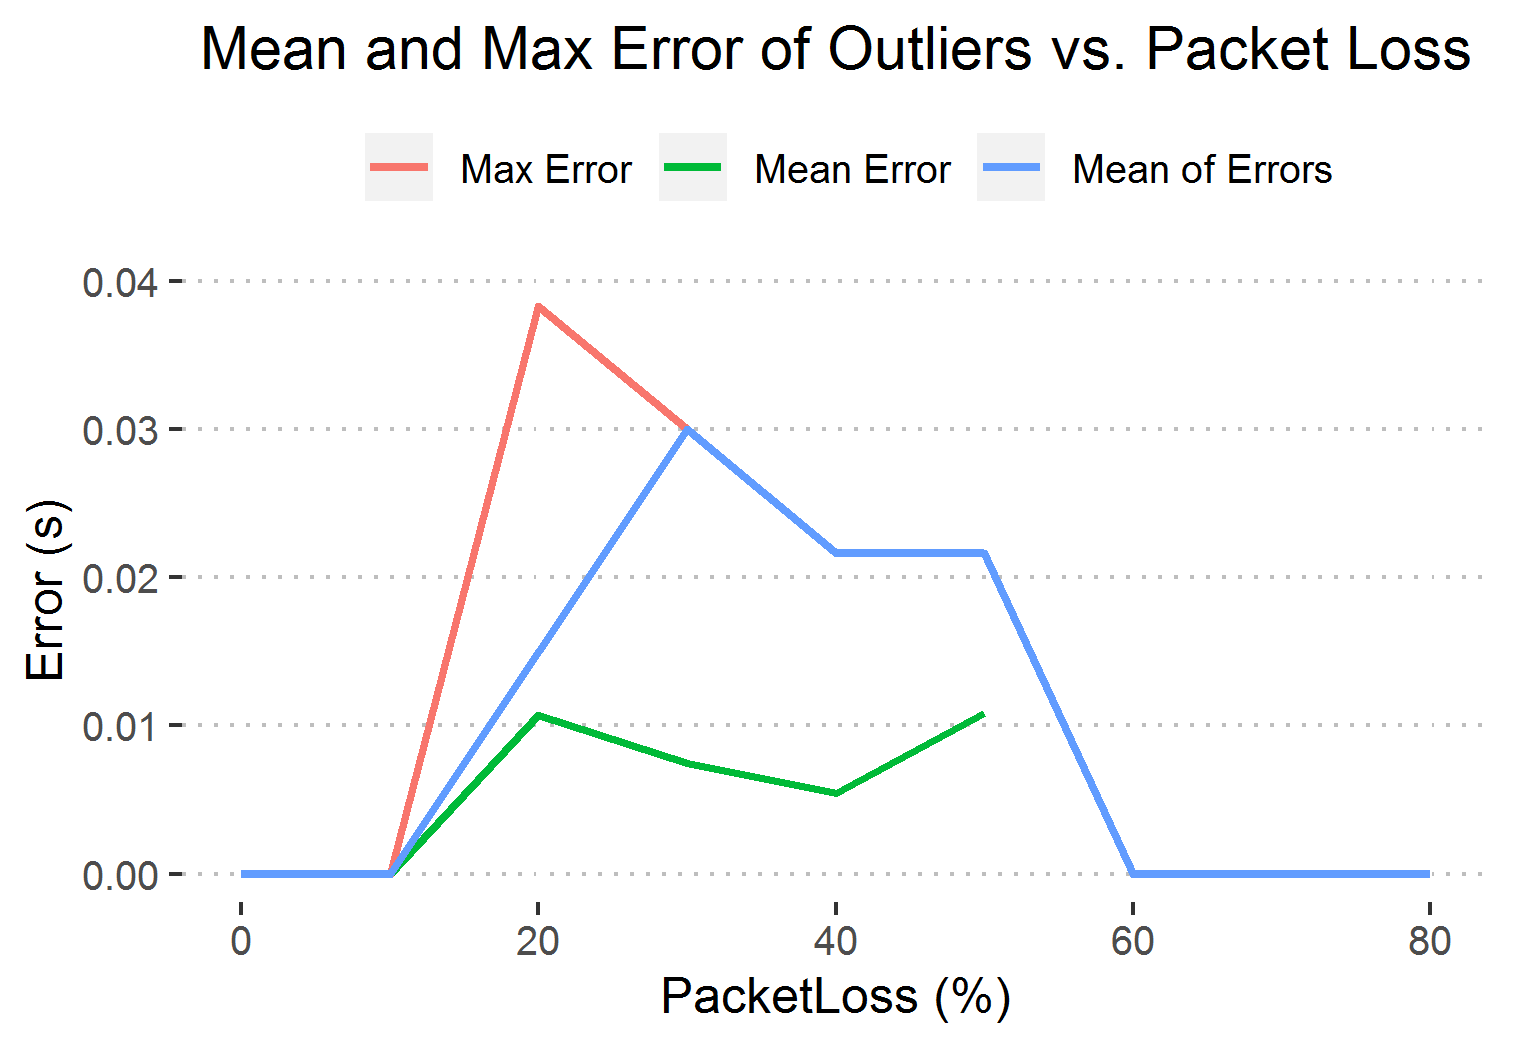
\includegraphics[width=\textwidth]{MeanMaxErrorVsLoss}
%\caption{The mean and max of collision errors with varying packet loss. As packet-loss increases from $10\%$ to $20\%$ the magnitude of errors sharply increases until above $60\%$ where all collisions are missed so there is no error.}
%\label{fig_MeanMaxErrorVsLoss}
%\end{figure}
%
%\begin{figure}
%\centering
%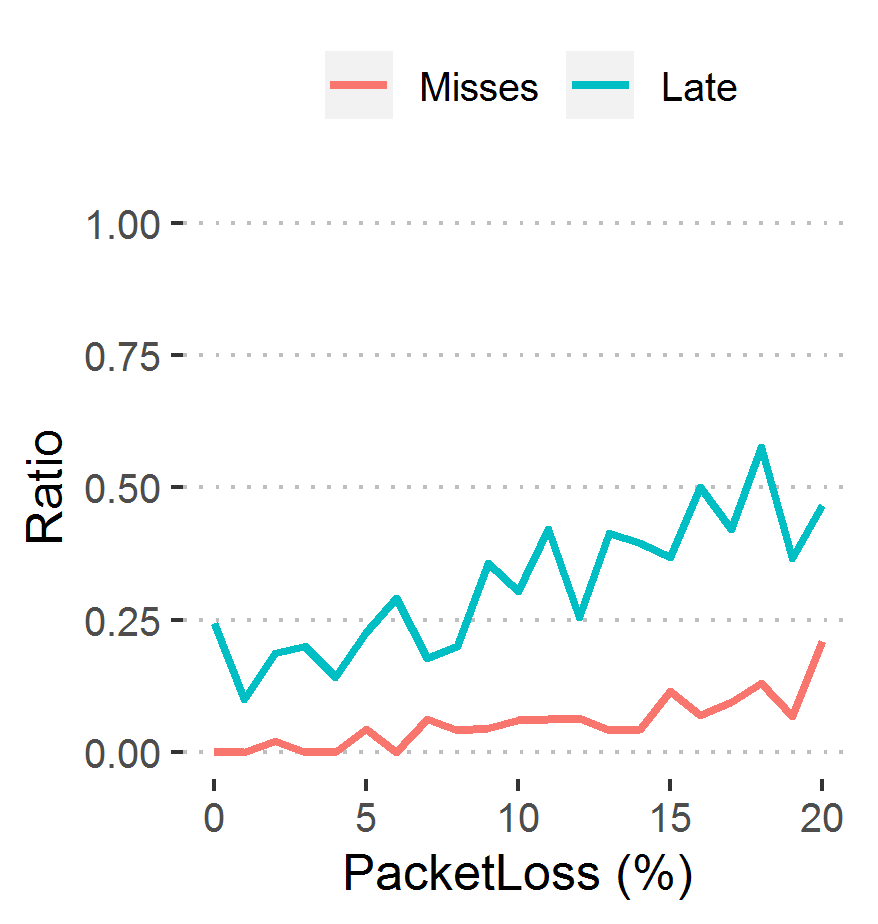
\includegraphics[width=\textwidth]{RatiosVsLoss}
%\caption{The ratios of erroneous collisions to correct collisions and missed collisions to total collisions with varying packet loss. As packet-loss increases from $10\%$ to $20\%$ the ratio of erroneous collisions to correct collisions sharply increases as does misses to total collisions. Above $60\%$ packet-loss, all collisions are missed.}
%\label{fig_RatiosVsLoss}
%\end{figure}

\subsubsection{Evaluation}
As packet-loss increases, late and erroneous collisions increase and late collisions increase in magnitude. This is due to messages being delayed as packets are lost and need to be re-sent by RakNet's reliability layer. Missed collisions begin to occur as soon as packet-loss exceeds $1\%$, but increase at a lower rate relative to late collisions. (Note, late collisions begin to occur from $0\%$, this is expected as all factors are set to be equal to their tolerances). These results demonstrate that AP is able to prevent $50\%$ of late collisions even in cases of packet-loss as high as (15\%) and prevent all missed collisions with up to $1\%$ packet-loss, which is much greater packet-loss than would be expected in practice (0.01\%) \cite{ThousandEyesCloudPerf2018}.
